\documentclass[titlepage]{jsarticle}

\usepackage{otf}

\usepackage{here}
\usepackage{array,booktabs} %表のためのarray環境
%数式用パッケージ
\usepackage{amsmath,amssymb}
\usepackage{mathtools}
\usepackage{cancel}
\usepackage{cases}
\usepackage{bm}
\usepackage{colortbl}
\usepackage{float}
\usepackage{subcaption}
%ファインマングラフ用パッケージ
\usepackage{feynmf}
%ハイパーリンクの設定
\usepackage[dvipdfmx]{graphicx}
\usepackage[dvipdfmx]{hyperref}
\usepackage{pxjahyper}
\hypersetup{
  colorlinks=false, % リンクに色をつけない設定
  bookmarks=true, % 以下ブックマークに関する設定
  bookmarksnumbered=true,
  pdfborder={0 0 0},
  bookmarkstype=toc
}

\newcommand{\Slash}[1]{{\ooalign{\hfil/\hfil\crcr\(#1\)}}}
\newcommand{\figref}[1]{\figurename\ref{#1}}
\newcommand{\tabref}[1]{\tablename\ref{#1}}

%\graphicspath{{./figure/}}

\begin{document}
%title
\title{課題研究P2\\J-PARC MLF  のミューオンビームを用いた\\ミューオン崩壊に関する諸量の測定}
\author{阿部倫史,池満拓司,小田川高大,田島正規\\羽田野真友喜,早川龍,三野裕哉}
\date{\today}
\maketitle
%目次
\tableofcontents
\newpage
%
% 句読点の統一
%\documentclass[titlepage]{jsarticle}

%\usepackage[dvipdfmx]{graphicx}

%数式用パッケージ
%\usepackage{amsmath, amssymb}
%\usepackage{mathtools}
%\usepackage{cancel}
%\usepackage{cases}
%\usepackage{bm}

%ファインマングラフ用パッケージ
%\usepackage{feynmf}

%ファインマンスラッシュ
%\newcommand{\Slash}[1]{{\ooalign{\hfil/\hfil\crcr\(#1\)}}}

%\title{課題研究P2\\J-PARC MLF  のミューオンビームを用いた\\ミューオン崩壊に関する諸量の測定}
%\author{阿部倫史,池満拓司,小田川高大,田島正規\\羽田野真友喜,早川龍,三野裕哉}
%\date{\today}

%\begin{document}

\section{序論}
本研究の目的はミューオンの崩壊現象を通して,標準模型,とくに弱い相互作用に関する各種の検証を行うことである.今回の実験で測定したい量は以下の三つである.

\begin{description}
\item[ミューオンの寿命]

ミューオンは弱い相互作用によって崩壊することが知られており,その寿命は標準模型によって計算されている.今回の実験ではミューオンビームを標的中で止めることで,ミューオンの寿命を測定し.その値を理論値と比較することで標準模型の検証を行う.
\item[ミッシェルパラメータ]

ミューオンの崩壊によって出てきた電子(陽電子)のエネルギースペクトルにおいて,ミッシェルパラメータと呼ばれるいくつかのパラメータを考えることができ,弱い相互作用の$V - A$ 理論ではこの値が決定されている.また,このエネルギースペクトルには$\cos \theta$ に比例する特徴的な項が存在し,これは弱い相互作用のパリティ対称性の破れを表している.今回の実験ではこのエネルギースペクトルを求めることでミッシェルパラメータの値を決定し,弱い相互作用のパリティ対称性の破れを確認するとともに,$V - A$ 理論の妥当性を検証する.
\item[$g$ 因子]

ミューオンの$g$ 因子の測定は標準模型の検証に用いられる典型的な実験の一つであり,とくに現在,標準模型を超えた物理の存在をも示唆する実験である.今回の実験ではミューオンビームを止める標的中に磁場をかけることでミューオンのスピンを歳差運動させ,$g$ 因子の測定をめざす.
\end{description}

また,これらの実験を通して粒子ビームを用いた素粒子実験に触れ,その方法を会得することを目的とする.

\section{理論}
本節では今回の実験で測定する物理量についてその背景にある理論を概説する.なお,詳しい計算等については一部については付録を見るか,あるいは参考文献を参照してほしい.以下,自然単位系($\hbar = c = 1$)を用いる.

\subsection{ミューオンとは}
ミューオン($\mu^{\pm}$)は1936年にAnderson らによって宇宙線から発見された,標準模型におけるレプトンの第二世代に属する素粒子である.$\mu^{\pm}$ は電子と同じ電荷$\pm e$,スピン$1/2$ を持ち,質量はその約$200$ 倍である.より正確には
	\[ m_{\mu} = 105.6583745 \pm 0.0000024~\mathrm{MeV}\]
と測定されている\cite{PDG}.
	
\subsection{ミューオンの寿命}
$\mu^{\pm}$ はほぼ100 \% の崩壊確率で次の崩壊を起こす\cite{PDG}.
\begin{eqnarray}
\mu^{-} \rightarrow e^{-} + \nu_{\mu} + \Bar{\nu}_{e}\\
\mu^{+} \rightarrow e^{+} + \Bar{\nu}_{\mu} + \nu_{\mu}
\label{eq:theory_muondecay}
\end{eqnarray}
今回の実験では$\mu^{+}$ を用いるので,以下$\mu^{+}$ についてその寿命を計算する.
	
\begin{figure}
\centering
\begin{fmffile}{feynmanzu1}
\begin{fmfgraph*}(120,80)

\fmfleft{mui}
\fmfright{numuo,eo,nueo}
				
\fmflabel{$\mu^{+}(p, r)$}{mui}
\fmflabel{$e^{+}(p', r')$}{eo}
\fmflabel{$\nu_e(q_{1}, r_{1})$}{nueo}
\fmflabel{$\bar{\nu}_{\mu}(q_{2}, r_{2})$}{numuo}
				
\fmf{fermion}{numuo,numumu,mui}
\fmf{boson,label=$W(k)$}{numumu,enue}
\fmf{fermion}{eo,enue}
\fmf{fermion}{enue,nueo}
				
\fmflabel{$\alpha$}{enue}
\fmflabel{$\!\!\!\beta$}{numumu}

\end{fmfgraph*}
\end{fmffile}
\vspace{10pt}
\caption{$\mu^{+}$ の崩壊のファインマン図}
\label{zu:muondecay}
\end{figure}
	
$\mu^{+}$ の崩壊は図\ref{zu:muondecay} のようなファインマン図で表される.標準模型(ワインバーグ=サラム理論)によればこの過程のファインマン振幅は
\begin{align}
\mathcal{M} = &-g_{W}^2\left[\Bar{u}(\bm{q_{1}})\gamma^{\alpha}(1 - \gamma_{5})v(\bm{p'})\right] \notag \\ 
&\times \frac{-(-g_{\alpha\beta} + k_{\alpha}k_{\beta}/m_{W}^2)}{k^{2} - m_{W}^2 + i\epsilon}\left[\Bar{v}(\bm{p})\gamma^{\beta}(1 - \gamma_5)v(\bm{q_{2}})\right]
\label{eq:theory_muondecayamp}
\end{align}%下の文章に対応する記号がありません
と書ける.ただし$p, q, k, \alpha, \beta$などは図\ref{zu:muondecay} に対応し,$g_{W}$ は弱い相互作用の結合定数である.その他の記法は付録に記載している通りである.ここで,$m_{W}^2$ が$k^2$ にくらべて十分大きいとし,$m_{W} \rightarrow \infty$の極限をとって計算すると,$V-A$理論の結果と一致する.この詳細な計算は付録に掲載するが結果として$\mu^+$ の寿命
\begin{equation}
\tau_{\mu} = \frac{192\pi^3}{G^{2} m_{\mu}^{5}}
\label{eq:thory_muonlifetime}
\end{equation}
が得られる.ここで$G$ はFermi 結合定数である.

実際の測定値としては
\[\tau_{\mu} = 2.1969811 \pm 0.0000022 \times 10^{-6}~\mathrm{s}\]
という値が得られている\cite{PDG}.
	
\subsection{ミッシェルパラメータ}
式\eqref{eq:theory_muondecay} で書かれる$\mu^{+}$ の崩壊で出てくる$e^{+}$ を考える.静止した$\mu^{+}$ が崩壊する時,運動量とエネルギーの保存から$e^{+}$ が持ちうる最大エネルギーは$m_{\mu}/2 \simeq 50~\mathrm{MeV}$ であり,完全に偏極された$\mu^{+}$ の崩壊を静止系で考えると,出てくる$e^{+}$ のエネルギー及び角度分布はミッシェルパラメータと呼ばれる四つのパラメータ$\rho, \eta, \xi, \delta$ を用いて次のようにあらわすことができる\cite{michel_parameter}.
\begin{align}
\frac{d^2\Gamma}{x^{2}dxd(\cos \theta)} \propto& \,\,(3 - 3x) + \frac{2}{3}\rho (4x - 3) \notag \\
&+ 3 \eta \,x_{0} \frac{1-x}{x} + \xi \cos \theta \left[(1 - x) + \frac{2}{3} \delta (4x - 3)\right]
\label{eq:theory_michel}
\end{align}
ここでニュートリノの質量や輻射補正は無視した.ただし,$\theta$ は$e^{+}$ の運動量と$\mu^{+}$ のスピンのなす角度であり,$x$ は$e^{+}$ のエネルギーの最大値が1 となるように規格化したものである.また,$x_0$ は$e^{+}$ のエネルギーが$m_{e}$ のときの$x$ の値であり,これは通常無視できるので第3 項は考えないことも多い.

$\theta = \pi/2$ の位置で,もしくは全$\theta$にわたって測定した場合にはスピンに関係する第4項が0となるため,第1 項,第2 項のみを考えればよい.このとき式\eqref{eq:theory_michel} から
\begin{equation}
\frac{d\Gamma}{x^{2}dx} \propto (3 - 3x) + \frac{2}{3}\rho (4x - 3)
\label{eq:theory_michel2}
\end{equation}
となる.

Lorentz 共変な相互作用においては$\rho = 0, 0.75, 1$ のいずれかになることが分かっている\cite{michel_interaction}.入射粒子数で規格化すると,結局$\Gamma$ は$\rho$ によらないので式\eqref{eq:theory_michel2} をそのまま描いて,測定で得られるグラフの形は図\ref{zu:michelpar} のいずれかのようになる.
\begin{figure}[htbp]
\centering
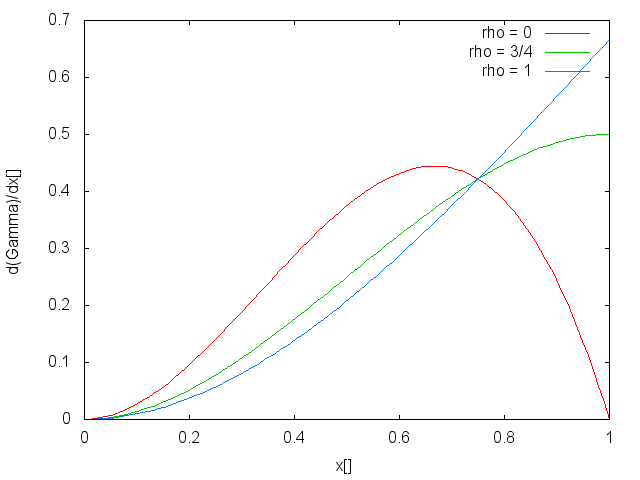
\includegraphics[width = 0.5\textwidth]{figure/abe/michelgraph.png}
\caption{Michel 崩壊の各$\rho$ に対するスペクトル}
\label{zu:michelpar}
\end{figure}
これらのグラフは大きく形が異なっているため,測定で得られたスペクトルを見ればある程度の相互作用の形を知ることができる.

特に,$V-A$ 理論では
\[ \rho = \xi\delta = \frac{3}{4},\, \eta = 0,\, \xi = 1 \]
となる.

また,実際には輻射補正を考えるとたとえば$\rho$ は$3 \sim 7$~\% ほど小さく測定されることが知られている.

現在のミッシェルパラメータの測定値は
\begin{align*}
\rho &= 0.74979 \pm 0.00026\\
\eta &= 0.057 \pm 0.034\\
\delta &= 0.75047 \pm 0.00034\\
\xi &= 1.0009^{+0.0016}_{-0.0007}
\end{align*}
である\cite{PDG}.
	
\subsection{ミューオンの$g$因子}
$\mu^{+}$ を含む,ディラック場で表されるようなフェルミ粒子の運動は次のDirac 方程式で記述される.
\begin{equation}
(i\Slash{\partial} - m)\psi(x) = 0
\label{eq:theory_dirac}
\end{equation}
ここで記法は付録と同じとする.

次に式\eqref{eq:theory_dirac} をもとにして外場としての電磁場$A_{\mu}$ が存在する状態での方程式を考える.U(1) 局所ゲージ対称性を課すと,共変微分$D_{\mu} = \partial_{\mu} + ieA_{\mu}$ を定義できて,
\begin{equation}
(i\Slash{D} - m)\psi(x) = 0
\label{eq:theory_diracwitha}
\end{equation}
となる.

ここから非相対論的近似を行うために,いままで用いてきた自然単位系$\hbar = c = 1$ から$\hbar$ と$c$ を復活させる.$A_{\mu} = (\phi, \bm{A})$ とおくと,
\begin{equation}
i\hbar\frac{\partial}{\partial t}\psi(x) = \left\{c\bm{\alpha}\cdot (\bm{p} - e\bm{A}) + \beta m c^{2} + e \phi\right\}\psi(x)
\label{eq:theory_diracwithaphi}
\end{equation}
となる.スピノル$\psi(x)$ を
\begin{equation}
\psi(x) = \begin{pmatrix}
\chi_{1} (x)\\
\chi_{2} (x)
\end{pmatrix} \exp \left( - i \frac{mc^{2}}{\hbar} t\right)
\end{equation}
と書き,式\eqref{eq:theory_diracwithaphi} に代入すると
\begin{align}
i\hbar\left( -i\frac{mc^{2}}{\hbar} + \frac{\partial}{\partial t}\right) \chi_{1} = c\bm{\sigma}\cdot(\bm{p} - e \bm{A})\chi_{2} + (mc^{2} + e\phi)\chi_{1} \label{eq:theory_chi1}\\ 
i\hbar\left( -i\frac{mc^{2}}{\hbar} + \frac{\partial}{\partial t}\right) \chi_{2} = c\bm{\sigma}\cdot(\bm{p} - e \bm{A})\chi_{1} - (mc^{2} - e\phi)\chi_{2} \label{eq:theory_chi2}
\end{align}

非相対論近似においては式\eqref{eq:theory_chi2} について時間微分項が無視でき,またスカラーポテンシャルによるエネルギーも無視できるので
\begin{equation}
\chi_{2} = \frac{1}{2mc}\bm{\sigma}\cdot(\bm{p} - e\bm{A})\chi_{1}
\end{equation}
となる.これを式\eqref{eq:theory_chi1} に代入し,$\sigma$ 行列に関する計算を行えば
\begin{equation}
i\hbar\frac{\partial}{\partial t}\chi_{1} = \left\{\frac{(\bm{p} - e\bm{A})^{2}}{2m} + e\phi - \frac{e\hbar\bm{\sigma}}{2m}\cdot\bm{B}\right\}\chi_{1}
\label{eq:theory_pauli}
\end{equation}
という,Pauli 方程式が得られる.ここで$\bm{B} = \nabla \times \bm{A}$ であり,磁束密度を表す.式\eqref{eq:theory_pauli} よりスピン$\hbar\bm{\sigma}/2$ がもつ磁気モーメントは軌道角運動量の場合の二倍であり,この場合$g$ 因子は2 であることがわかる.

上のような計算を行えばDirac 方程式からミューオンの$g$ 因子は2 と求まる.QED (量子電磁力学)による考察を行うと,その結果$g$ 因子には補正がかかることが分かっている.$g$ 因子のこの2 からのずれを異常磁気能率 (anomalous magnetic moment) と呼ぶ.例えば二次の摂動において異常磁気能率に寄与する過程はSchwinger によって説明された図\ref{zu:vertexcorr} で表される過程である.

\begin{figure}[h]
\centering
\begin{fmffile}{feynmanzu2}
\begin{fmfgraph*}(100,80)
				
\fmfleft{mui}
\fmfright{muo}
\fmfbottom{ai}
				
\fmflabel{$\mu$}{mui}
\fmflabel{$\mu$}{muo}
\fmflabel{$\gamma$}{ai}
				
\fmf{fermion}{mui,muig,muia}
\fmf{boson}{ai,muia}
\fmf{boson,left=0.5,tension=0.2}{muig,muog}
\fmf{fermion}{muia,muog,muo}
				
\end{fmfgraph*}
\end{fmffile}
\vspace{10pt}
\caption{二次の摂動における異常磁気能率への寄与過程}
\label{zu:vertexcorr}
\end{figure}

図\ref{zu:vertexcorr} で表される過程の寄与は$\alpha/2\pi$ (ここで$\alpha$ は微細構造定数$1/137$)である.

このような寄与をQED のより高次の摂動についても考えることができ,また一方でQED のレプトニックな過程以外の$W, Z$ ボソンを含む電弱理論に関して,あるいはハドロンが関与する過程に関しても考えることができる.このようにして,さまざまな相互作用を加味した異常磁気能率の理論値\cite{g-2_theory}は
\[a_{\mu} = (g -2)/2 = 116591804(51) \times 10^{-11}\]
であり,その測定値\cite{g-2_experiment}は
\[a_{\mu} = 116592089(63) \times 10^{-11}\]
である.%\cite{}
これらはQED の正しさを証明する一方で,標準模型の理論値とも$3\sigma$ 以上の有意な差があり,ここに新たな物理があることが期待されている.実際,未発見の粒子が存在して上に述べたような過程の他にその粒子の寄与を考えると,計算するべきファインマン図が増え,その分異常磁気能率に対する計算値も変わることになる.

そのため,$g$ 因子の測定は新しい物理の探索を目的として現在の素粒子物理学実験においてもっとも精密な計算と測定が行われている例である.

\section{実験原理}
本節では今回の実験の原理について説明する.今回の実験ではミューオン ($\mu^{+}$) ビームを用いてミューオンの崩壊寿命,ミッシェルパラメータ,そして$g$ 因子を測定する.そのために用いる検出器としてNaI (Tl) シンチレータとプラスチックシンチレータを採用する.なお,ミューオンビームの詳細は次節に含めている.

\subsection{寿命測定の原理}
ミューオンビームは標的で止められる.静止したミューオンは式\eqref{eq:thory_muonlifetime}の寿命を持つため,
\begin{equation}
\frac{dN_\mu}{dt} = -\frac{1}{\tau_\mu} N_{\mu}
\end{equation}
に従い崩壊し,この際にミューオンはほぼ100~\%の確率で陽電子を一つ出す.崩壊して出てくる陽電子の数は崩壊したミューオンの数と一致し
\begin{equation}
\frac{dN}{dt} = N_0 \exp{\left(-\frac{t}{\tau_\mu}\right) }
\end{equation}
で減少する.つまり陽電子を検出し,計数の時間変化を指数関数でフィッティングすれば寿命を求めることができる.

\subsection{ミッシェルパラメータ測定の原理}
今回はミッシェルパラメータのうち$\rho$ を測定するための実験を行なった.理論の節と述べたように$\rho$ の測定にはミュオンのスピンの向きに対して,$\theta = \pi / 2$ の位置で観測,または無偏極のミューオンのエネルギーを測定しなくてはならない.

ミュオンビームは進行方向にスピン偏極しているため,標的からビーム方向に対して$90^{\circ}$ の向きに検出器を設置してエネルギーを測定,得られたエネルギースペクトルを式\eqref{eq:theory_michel2} でフィッティングすれば,$\rho$ を求めることができる.この際,最大50~MeVの陽電子が出るので,50~MeV陽電子を止めきるような検出器が要求される.また実際には,$90^{\circ}$ 方向に検出器を置くことが困難だったことやデータ量の関係から,後述する$g$ 因子測定のデータを利用して,全スピン方向で積分した無偏極ミューオンとして$\rho$ を求めた.また,この解析によりスピン部分のデータが得られたため,最終的にはミッシェルパラメータの$\xi,\;\delta$ の解析も行った.

\subsection{$g$ 因子測定の原理}
ミュオンのスピンは磁場中で歳差運動をする.一様磁場中において,磁場方向を$z$軸とすると,磁場とスピンの相互作用のハミルトニアンは,
\begin{equation}
\hat{H} = - g \frac{e}{2m_\mu} \hat {\textsl{\textbf {S}}} \cdot \textsl{\textbf {B}} = - g \frac{e}{2m_\mu}  \hat{S_z} B
\end{equation} 
であるので,Heisenberg方程式より,
\begin{equation}
\frac{d\hat{S_x}}{dt} =  g \frac{eB}{2m_\mu}\hat{S_y} 
\end{equation} 
\begin{equation}
\frac{d\hat{S_y}}{dt} = - g \frac{eB}{2m_\mu}\hat{S_x} 
\end{equation} 
\begin{equation}
\frac{d\hat{S_z}}{dt} = 0 
\end{equation} 
を得る.スピン初期状態を
\begin{equation}
\langle \textsl{\textbf {S}}(t=0)\rangle = (C,0,0)
\end{equation} 
とすれば,
\begin{equation}
\langle S_x \rangle= C\cos{(g\frac{eB}{2m_\mu}t)}
\end{equation}
\begin{equation}
\langle S_y \rangle= -C\sin{(g\frac{eB}{2m_\mu}t)}
\end{equation}
とスピンが$xy$平面内で回転することがわかり,その角速度$\omega$は,
\begin{equation}
\omega = g\frac{eB}{2m_\mu}
\end{equation}
となる.式\eqref{eq:theory_michel} の通り陽電子はミューオンのスピンの方向に出やすいので,磁場を通した標的でミューオンビームを止めると,陽電子の計数は指数的な減少に周期$2\pi / \omega$ の振動が加わったものになる.よってその周期から$g$ 因子を求めることができる.

\subsection{検出器サイズの見積もり}
今回の実験ではミューオンの崩壊の際に放出される陽電子を測定するが,この陽電子の最大エネルギーはおよそ50~MeVである事を前節で確認した.
もし検出器に50~MeVの陽電子が物質に入射すると,制動放射と対生成による電磁シャワーを形成する.今回の検出器は全吸収型のカロリメータとして設計したため,その電磁シャワーが検出器の寸法内に収まるように設計しなければならない.電磁シャワーの広がりはその内部にシャワーのエネルギーの90~%が含まれるような長さで記述され,その長さをモリエール半径$R_\mathrm{M}$ と呼ぶ.モリエール半径は次のように定義される.
\begin{equation}
R_\mathrm{M} = L_\mathrm{rad}\frac{21.2~\mathrm{MeV}}{E_\mathrm{c}}
\end{equation}
ここで$L_\mathrm{rad}$ は放射長,$E_\mathrm{c}$ はcritical energy である.NaI およびプラスチックシンチレータ (PS) における$L_{\rm rad}$ と$E_\mathrm{c}$ ,$R_\mathrm{M}$ の値を表\ref{tab:abe_rm} に示す.
\begin{table}[hbtp]
\centering
\caption{物質ごとの$L_\mathrm{rad}$と$E_\mathrm{c}$,およびモリエール半径$R_\mathrm{M}$}
\begin{tabular}{cccc}\toprule
物質 & $L_\mathrm{rad}~[\mathrm{cm}]$ & $E_\mathrm{c}~[\mathrm{MeV}]$ & $R_\mathrm{M}~[\mathrm{cm}]$ \\ \midrule
NaI & 2.59 & 17.4 & 3.2 \\
PS & 42.9 & 109 & 8.34 \\ \bottomrule
\end{tabular}
\label{tab:abe_rm}
\end{table}
この値から,検出器の横幅はNaIは5~cm,プラスチックシンチレータは10~cm程度の半径でよいと見積もった.なお実際にはGeant4 のシミュレーション結果も用いて,奥行き方向の長さも含めた検出器サイズを決定した.
% 奥行き方向に関する理論はなかったということ?
%ーLeoに乗っている奥行き方向に関する簡単なモデルではよい計算結果は出ないです,Leoで次に書いてあるのもシミュレーションなのでシャワーの奥行きについての理論的見積もりはないとしました
\newpage

\section{シミュレーション}%このセクションには大したことが書いてないけどいる?(05.30 Odagawa)
本節では前節で述べた実験原理を基に各種シミュレーションを行い,セットアップの詳細やジオメトリーの決定を行う.標的や検出器内での電磁相互作用の各種シミュレーションについてはGeant4 を用い,磁場のシミュレーションにはFEMM を用いた.
	
\subsection{Geant4 を用いたモンテカルロシミュレーション}
Geant4 (for Geometry and Tracking) は物質中での粒子の運動をモンテカルロシミュレーションするためのツールキットでありCERNなどによって開発され,Geant4 Collaboration によって管理されている.高エネルギー物理学分野をはじめ核物理学や,加速器物理,医療などの分野で広く用いられており,LHC での様々な実験やT2K 実験でも用いられている.今回の我々の実験では,Geant4 を用いて検出器の設計や,コリメータの寸法の調節,またそれらのシミュレーション結果を用いての解析手法の開発などを行った.%cite{}

\subsection{FEMM}
FEMM (Finite Element Method Magnetics) は有限要素法を用いて2 次元軸対称な電磁場や熱,電流などのシミュレーションを行うことができるソフトである.FEMM は線形および非線形な静磁場問題に対応しており,また,さまざまな境界条件を用いることができる.今回の我々の実験では$g$ 因子を測定する際の均一な磁場を作成するためにFEMM を用いたシミュレーションを行った.

%\end{document}

%\documentclass[]{jsarticle}

%\usepackage[dvipdfmx]{graphicx}
%\usepackage[dvipdfmx]{color}

%\usepackage{amsmath, amssymb}
%\usepackage{mathtools}
%\usepackage{cancel}
%\usepackage{cases}
%\usepackage{bm}

%\usepackage{here}
%\usepackage{colortbl}

%\begin{document}

%----------ここから-------------------
%----------ミューオンビーム-------------------
\section{実験方法}

\subsection{MLF ミューオンビーム}

\subsubsection{加速器科学インターンシップの利用}
KEK が学部3 回生以上を対象に行っている加速器科学インターンシップを利用することにより,ロシアの実験チームの $g - 2$ Beam Profile Monitor に関する実験のパラサイト実験という形でMLF ミューオンビームを利用できることを知った.ミューオンビームの性能を踏まえて可能な測定量および測定方法を考え実験の準備を行い,そのインターンシップを用いて実際のMLF ミューオンビームを用いて測定を行った.

 \subsubsection{表面ミューオン}
 MLF では炭素原子核に高エネルギーの陽子を衝突させることによってパイオンを生成し,パイオンが崩壊して得られるミューオンを利用している.炭素標的から飛び出したパイオンが超伝導ソレノイド磁石内部で崩壊することによって得られるミューオンは崩壊ミューオンと呼ばれるが,今回利用したのは炭素標的の表面に静止した$\pi^{+}$ 中間子の崩壊によって得られる$\mu ^{+}$ で,これは表面ミューオンと呼ばれる.この表面ミューオンは静止したパイオンから生じているため 100~\% のスピン偏極を持っており,非常にエネルギーが低く一定であるという特徴を有する.表面ミューオンがスピン偏極を持つのは弱い相互作用による崩壊で生じる際に,ニュートリノはヘリシティーが左巻きのもののみが結合することに由来する.なお炭素標的の表面で静止した$\mu^-$ は原子核に捕獲されるため,取り出すことはできない.

表面ミューオンビームラインの性能は表\ref{muon1} のとおりで,シングルバンチ(短時間のミューオンの集まり)のミューオンビームが$25~\mathrm{Hz}$ でやってくる.ビームの広がりのプロファイルは図\ref{muon2} のとおりである.%要表記確認

\begin{figure}[H]
\centering
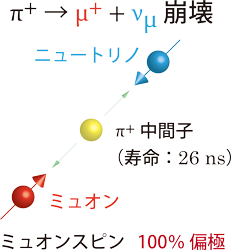
\includegraphics[width=0.4\textwidth]{figure/hayakawa/decay_pion.png}
\caption{$\pi^{+}$ 中間子の崩壊\cite{aboutmuon}}
\end{figure}

\begin{table}[H]
\caption{表面ミューオンビームラインの性能}
\label{muon1}
\centering
\begin{tabular}{cc}\toprule
ビームエネルギー & 4.1~MeV \\ \midrule
侵入長 & $\sim$ 0.2~mm \\ \midrule
エネルギー分布 & $\sim$ 15~\% \\ \midrule
パルス幅 (FWHM) & $\sim$ 100~ns \\ \midrule
ビームサイズ & 30~mm $\times$ 40~mm \\ \midrule
ビーム強度 & 3 $\times$ $10^7~/\mathrm{s}$ \\ \midrule
ポート数 & 2 \\ \bottomrule
\end{tabular}
\end{table}
   
\begin{figure}[H]
\centering
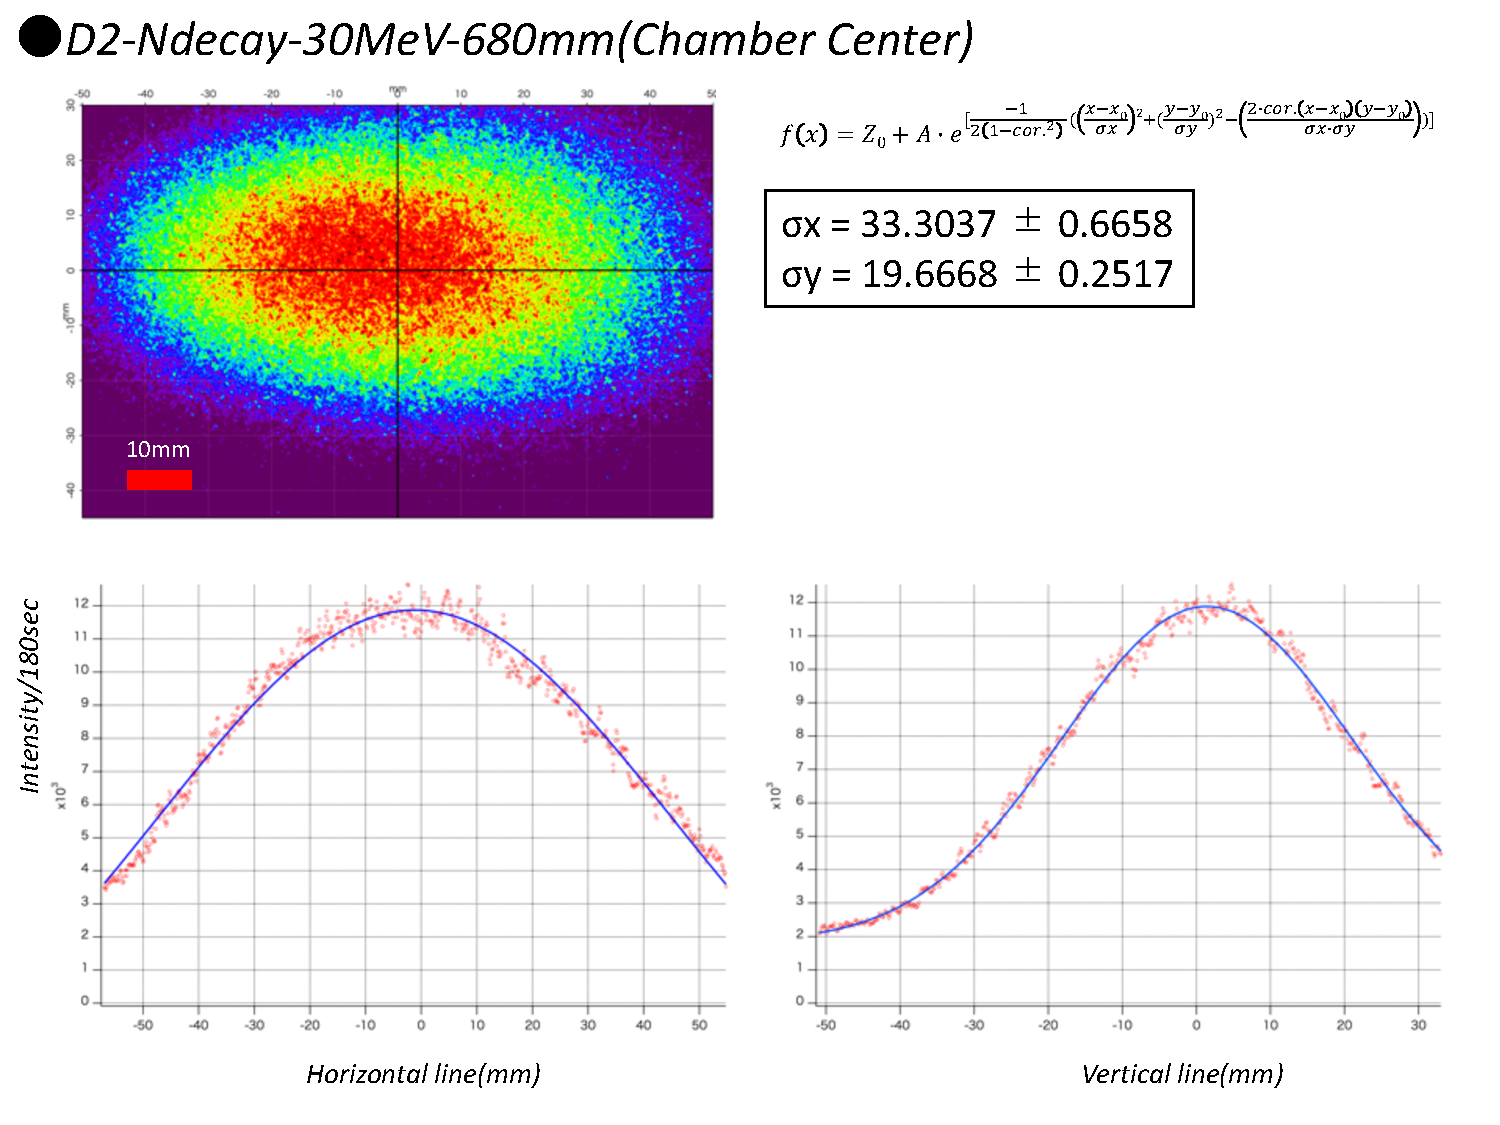
\includegraphics[width=0.8\textwidth]{figure/hayakawa/profile.pdf}
\caption{ミューオンビームの広がり(単位:$\mathrm{mm}$)}
\label{muon2}
\end{figure}

\subsection{測定量と検出器}

\subsubsection{実験概要}

今回の実験ではミューオンの寿命,ミッシェルパラメータ,$g$ 因子を測定する.基本的な実験の流れとしては,
\begin{itemize}
\item ビームラインから $\mu ^{+}$ が出て来る
\item ターゲットに止められた $\mu ^{+}$ が $e^{+}$ に崩壊する
\item 検出器で時間情報・エネルギー情報を測定する
\end{itemize}
という順序になる.測定の時間情報は寿命と$g$ 因子の測定,エネルギー情報はミッシェルパラメータの測定と各解析に対して独立に必要である.そのためにそれぞれの測定を中心に行う検出器として,時間分解能に優れたプラスチックシンチレータ(PS) 検出器および,エネルギー分解能に優れたNaI シンチレータ検出器の二種類の検出器を作成した.    
\begin{figure}[H]
\centering
\includegraphics[width=1\textwidth]{figure/hayakawa/lifetime.png}
\caption{実験概要}
\end{figure}

\subsubsection{検出器サイズの見積}

図 \ref{PS_sim} はGeant4 で行ったPS 検出器の体積シミュレーションである.検出器サイズの縦横は $20~\mathrm{cm}$ で固定し,奥行きを $20~\mathrm{cm}$ から$24~\mathrm{cm}$ まで変化させた直方体状のPS シンチレータに測定すべき最大のエネルギーである$50~\mathrm{MeV}$ の陽電子を入射させた.その際に検出器に落としたエネルギーをヒストグラムに示している.奥行きが$24~\mathrm{cm}$ 以下では$50~\mathrm{MeV}$ より下にピークが存在し,電磁シャワーが寸法内に収まらず陽電子のエネルギー充分に検出器に落とせていないことが分かる.一方,奥行きを$24~\mathrm{cm}$ 以上に増やしても,漏れるエネルギーが光子によるものの影響のためほとんど落とすエネルギーは変わらない.つまりこれ以上大きくしても効率が悪く,また基本的には$50~\mathrm{MeV}$ 程度のエネルギーを落としているため,奥行きは$24~\mathrm{cm}$ あれば十分であると決定した.
\begin{figure}[H]
\centering
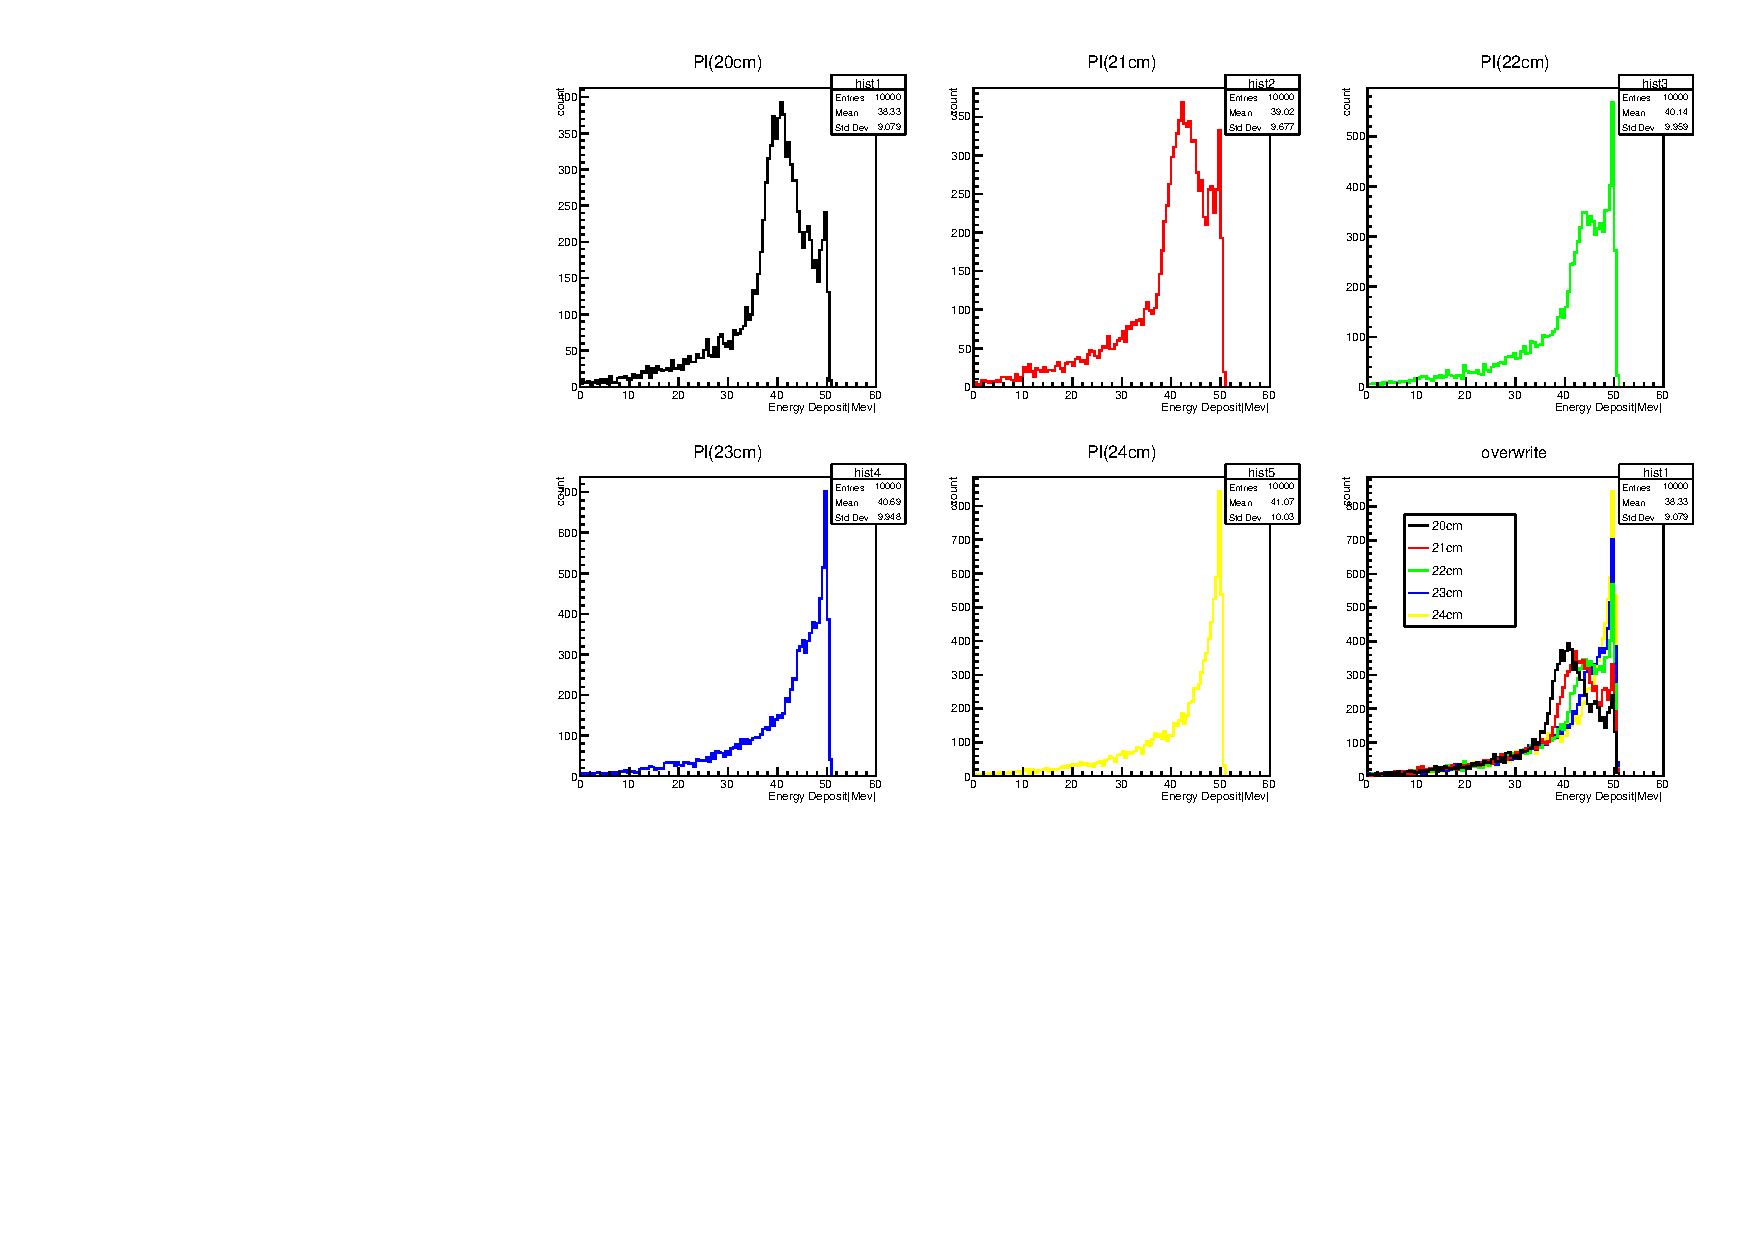
\includegraphics[width=0.6\textwidth,angle=-90]{figure/hayakawa/pl_20_24.pdf}
\caption{PS検出器の体積シミュレーション}
\label{PS_sim}
\end{figure}

図 \ref{NaI_sim} はNaI 検出器の体積シミュレーションである.NaI は光電子増倍管 (PMT) の接続された既製品を利用したため,既製品をどのように並べるべきか確認するために縦横の幅を変えながら同様のシミュレーションを行った.

\begin{figure}[H]
\centering
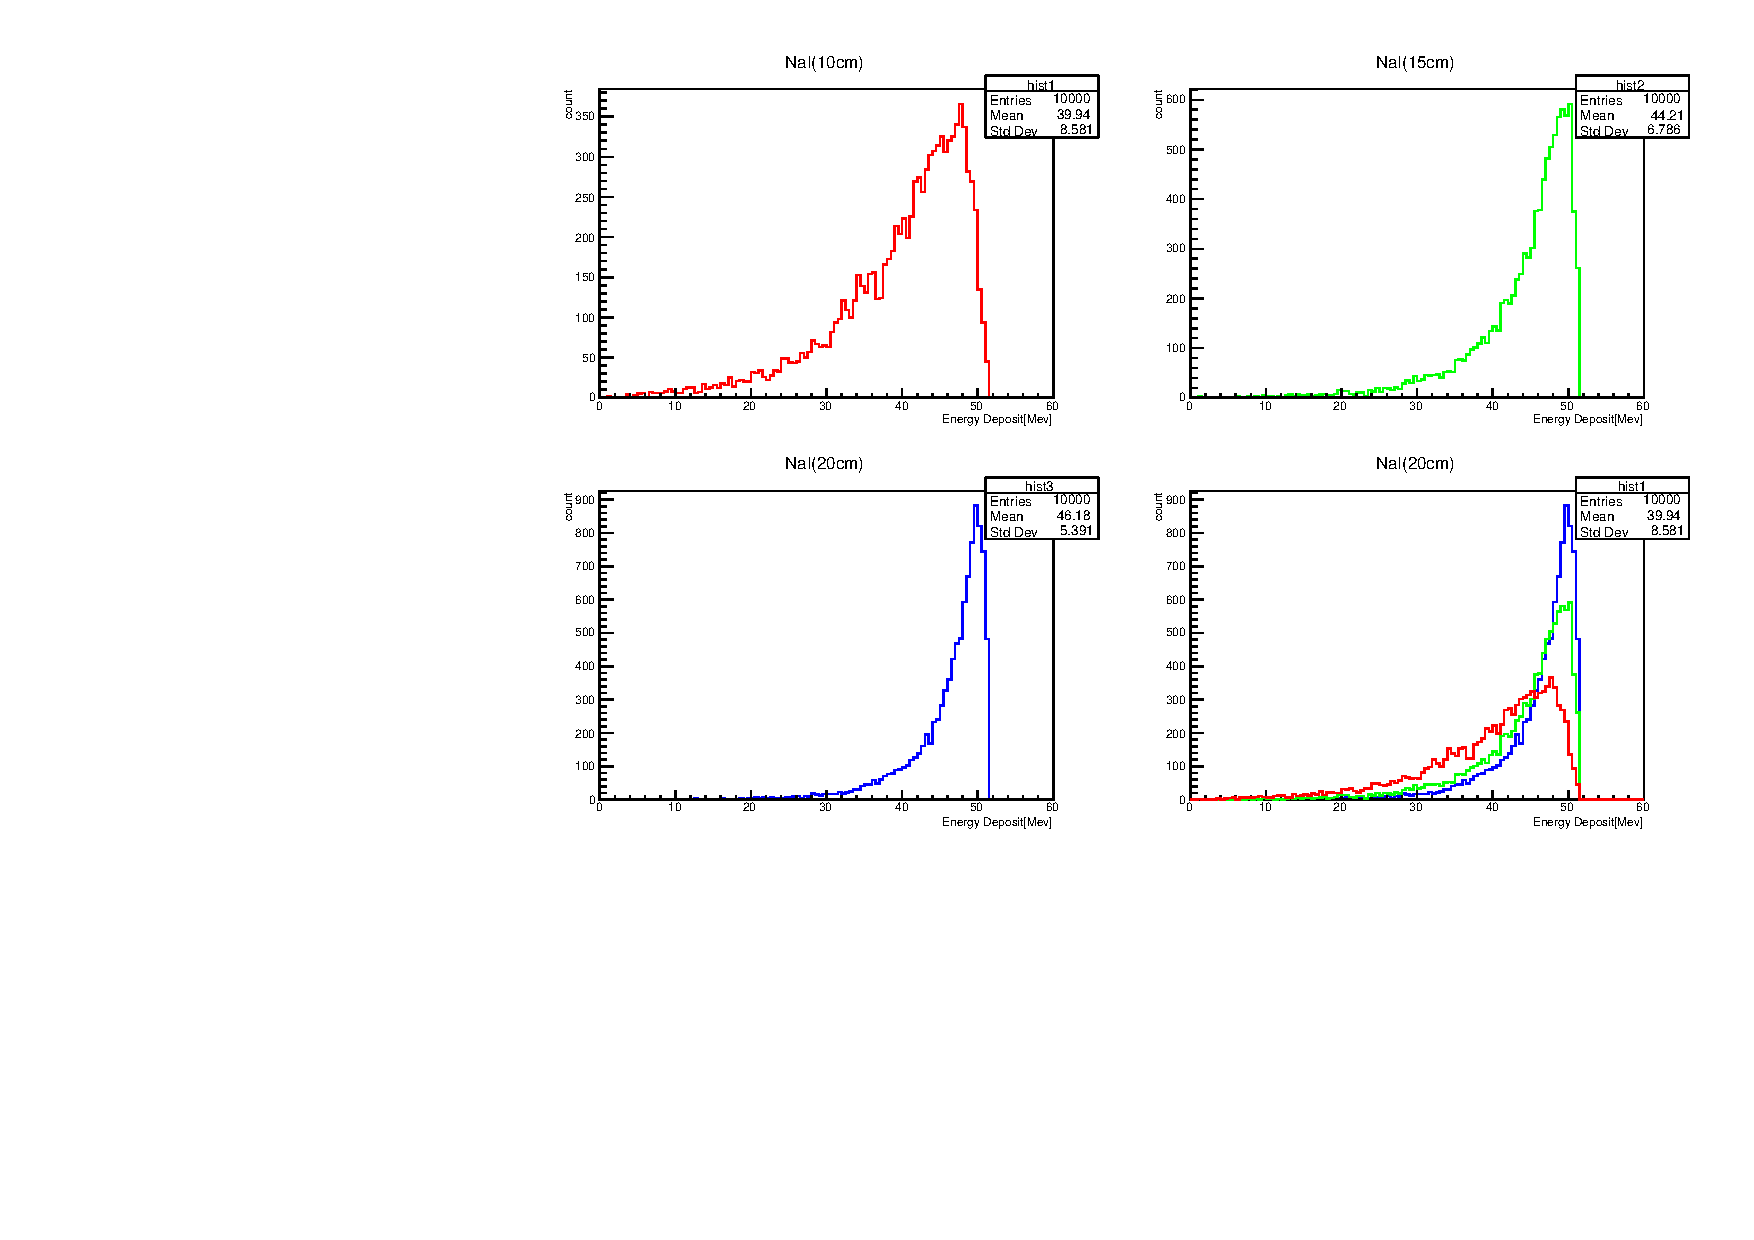
\includegraphics[width=0.55\textwidth,angle=-90]{figure/hayakawa/NaI_10_20.pdf}
\caption{NaI 検出器の体積シミュレーション}
\label{NaI_sim}
\end{figure}

\subsection{検出器の製作}

\subsubsection{PS 検出器の製作}
光ファイバー読み出しの板を並べることで,縦横$20~\mathrm{cm}$ ,奥行き$24~\mathrm{cm}$ の体積のPS 検出器を作成した.

\begin{figure}[H]
\centering
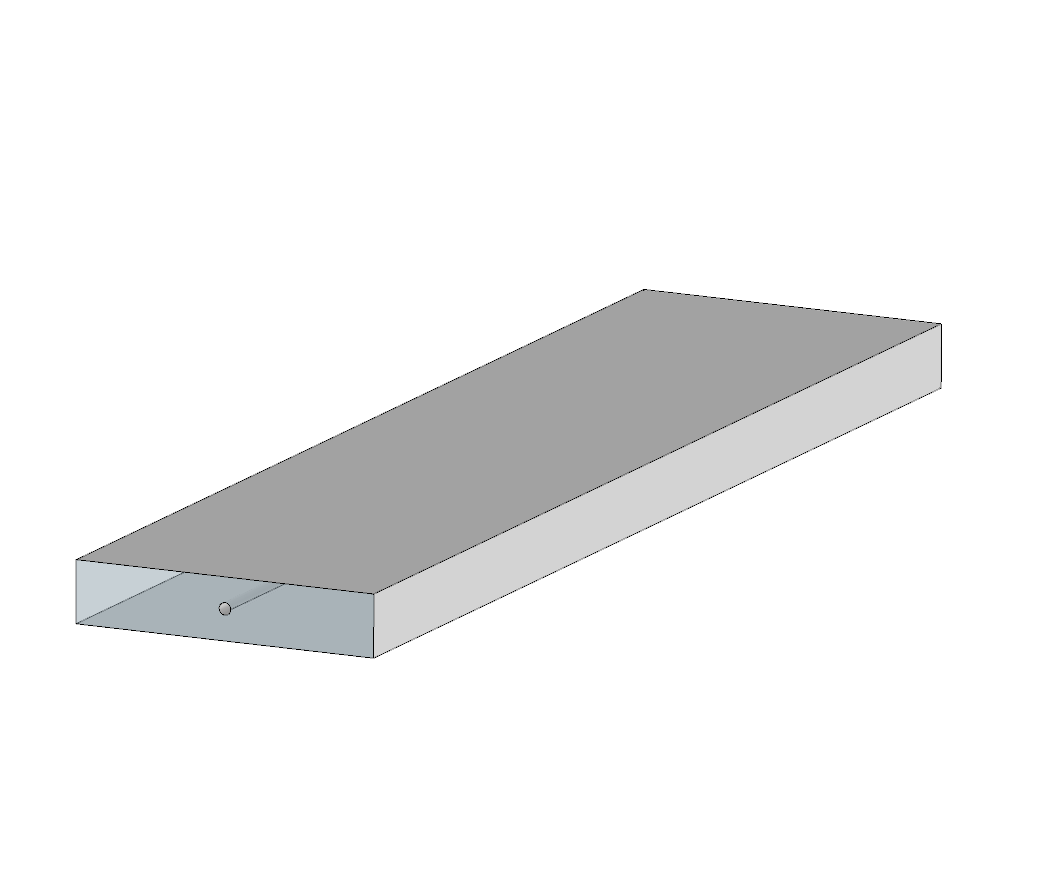
\includegraphics[width=0.3\textwidth]{figure/hayakawa/psmd.png}
\caption{PS 板}
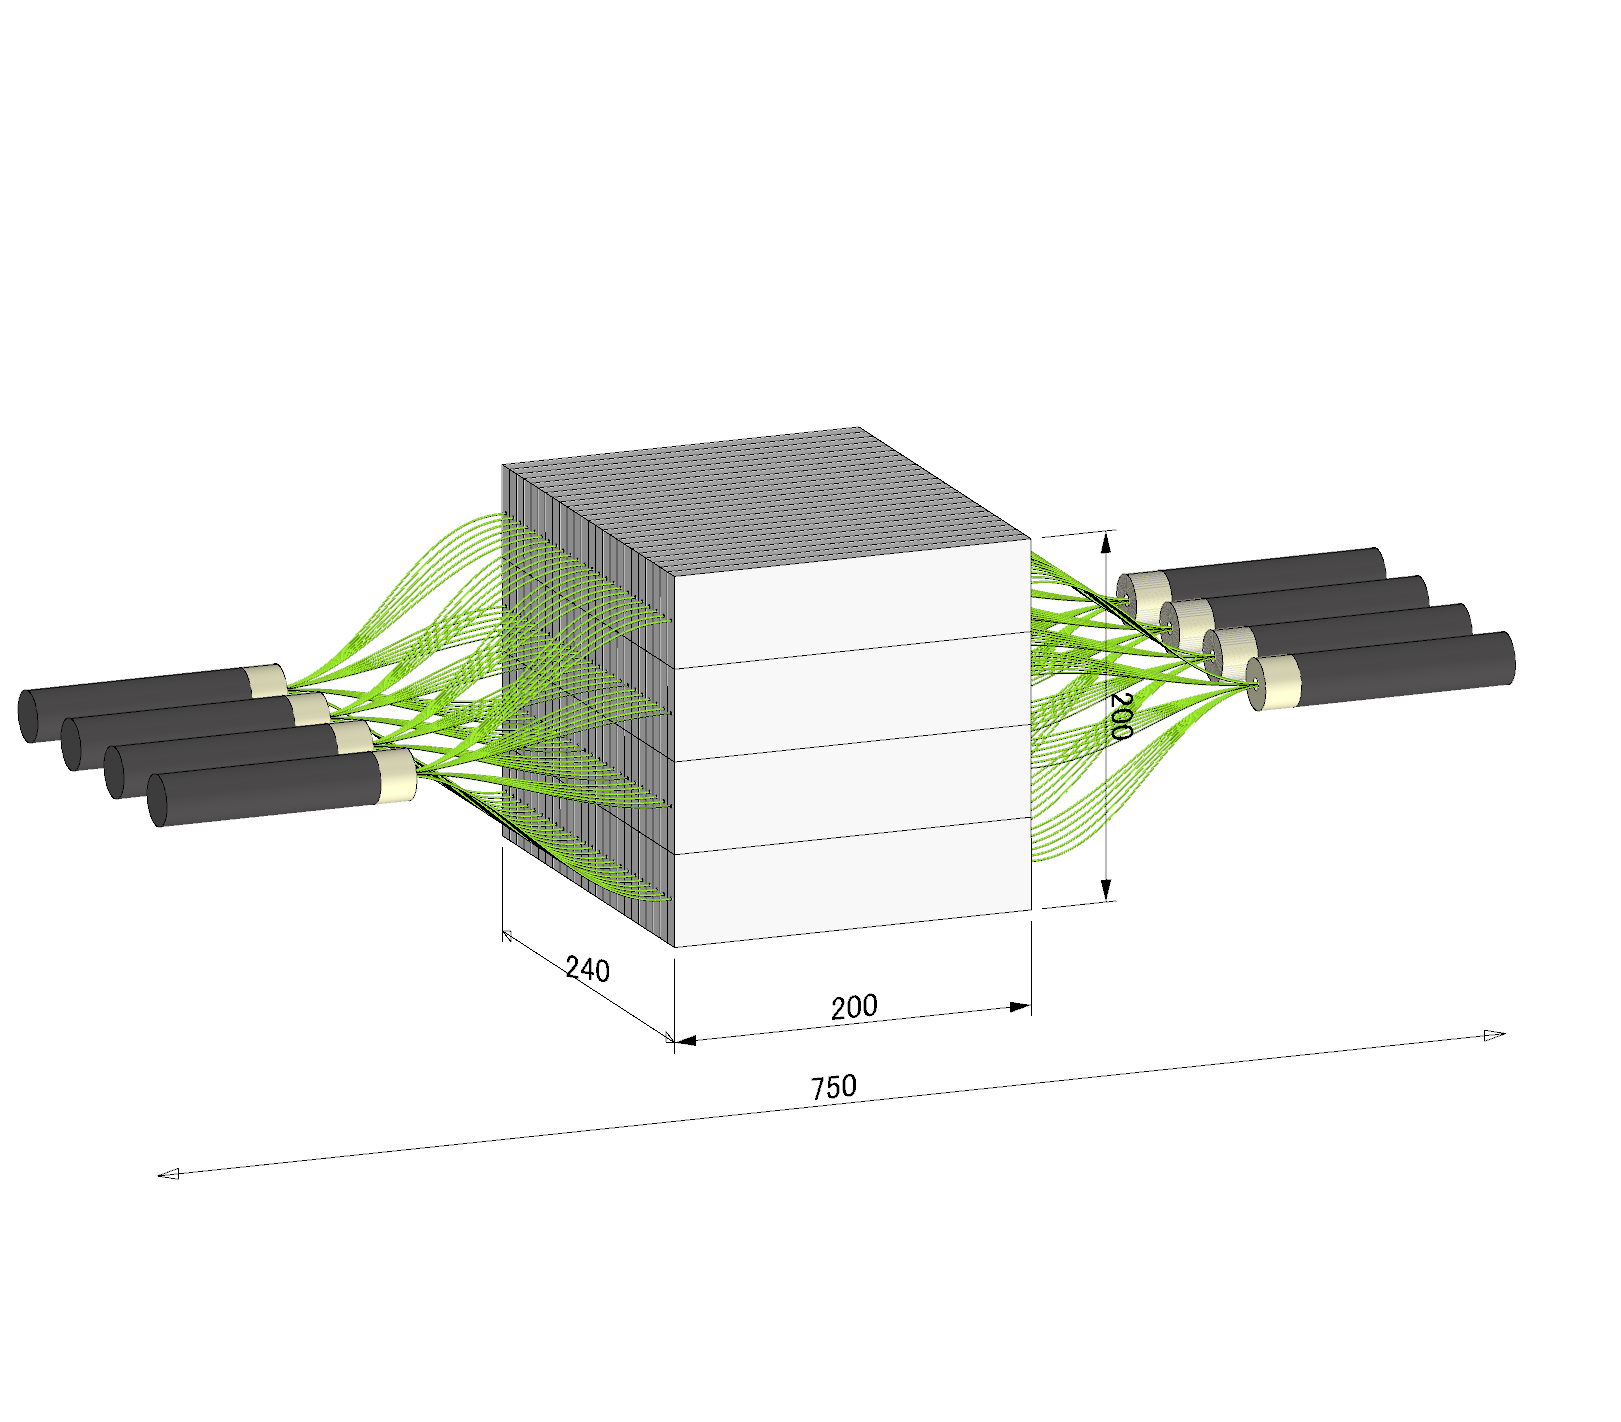
\includegraphics[width=0.8\textwidth]{figure/hayakawa/p7.png}
\caption{PS 検出器寸法}
\label{PS_sunpou}
\end{figure}

以下の順序で検出器を作成した.
\begin{itemize}
\item 厚み$6~\mathrm{cm}$ に束ねたものを$4$ セット作成した
\item 光ファイバーの片端をクッキーを用いて光学セメントで固定した
\begin{figure}[H]
\centering
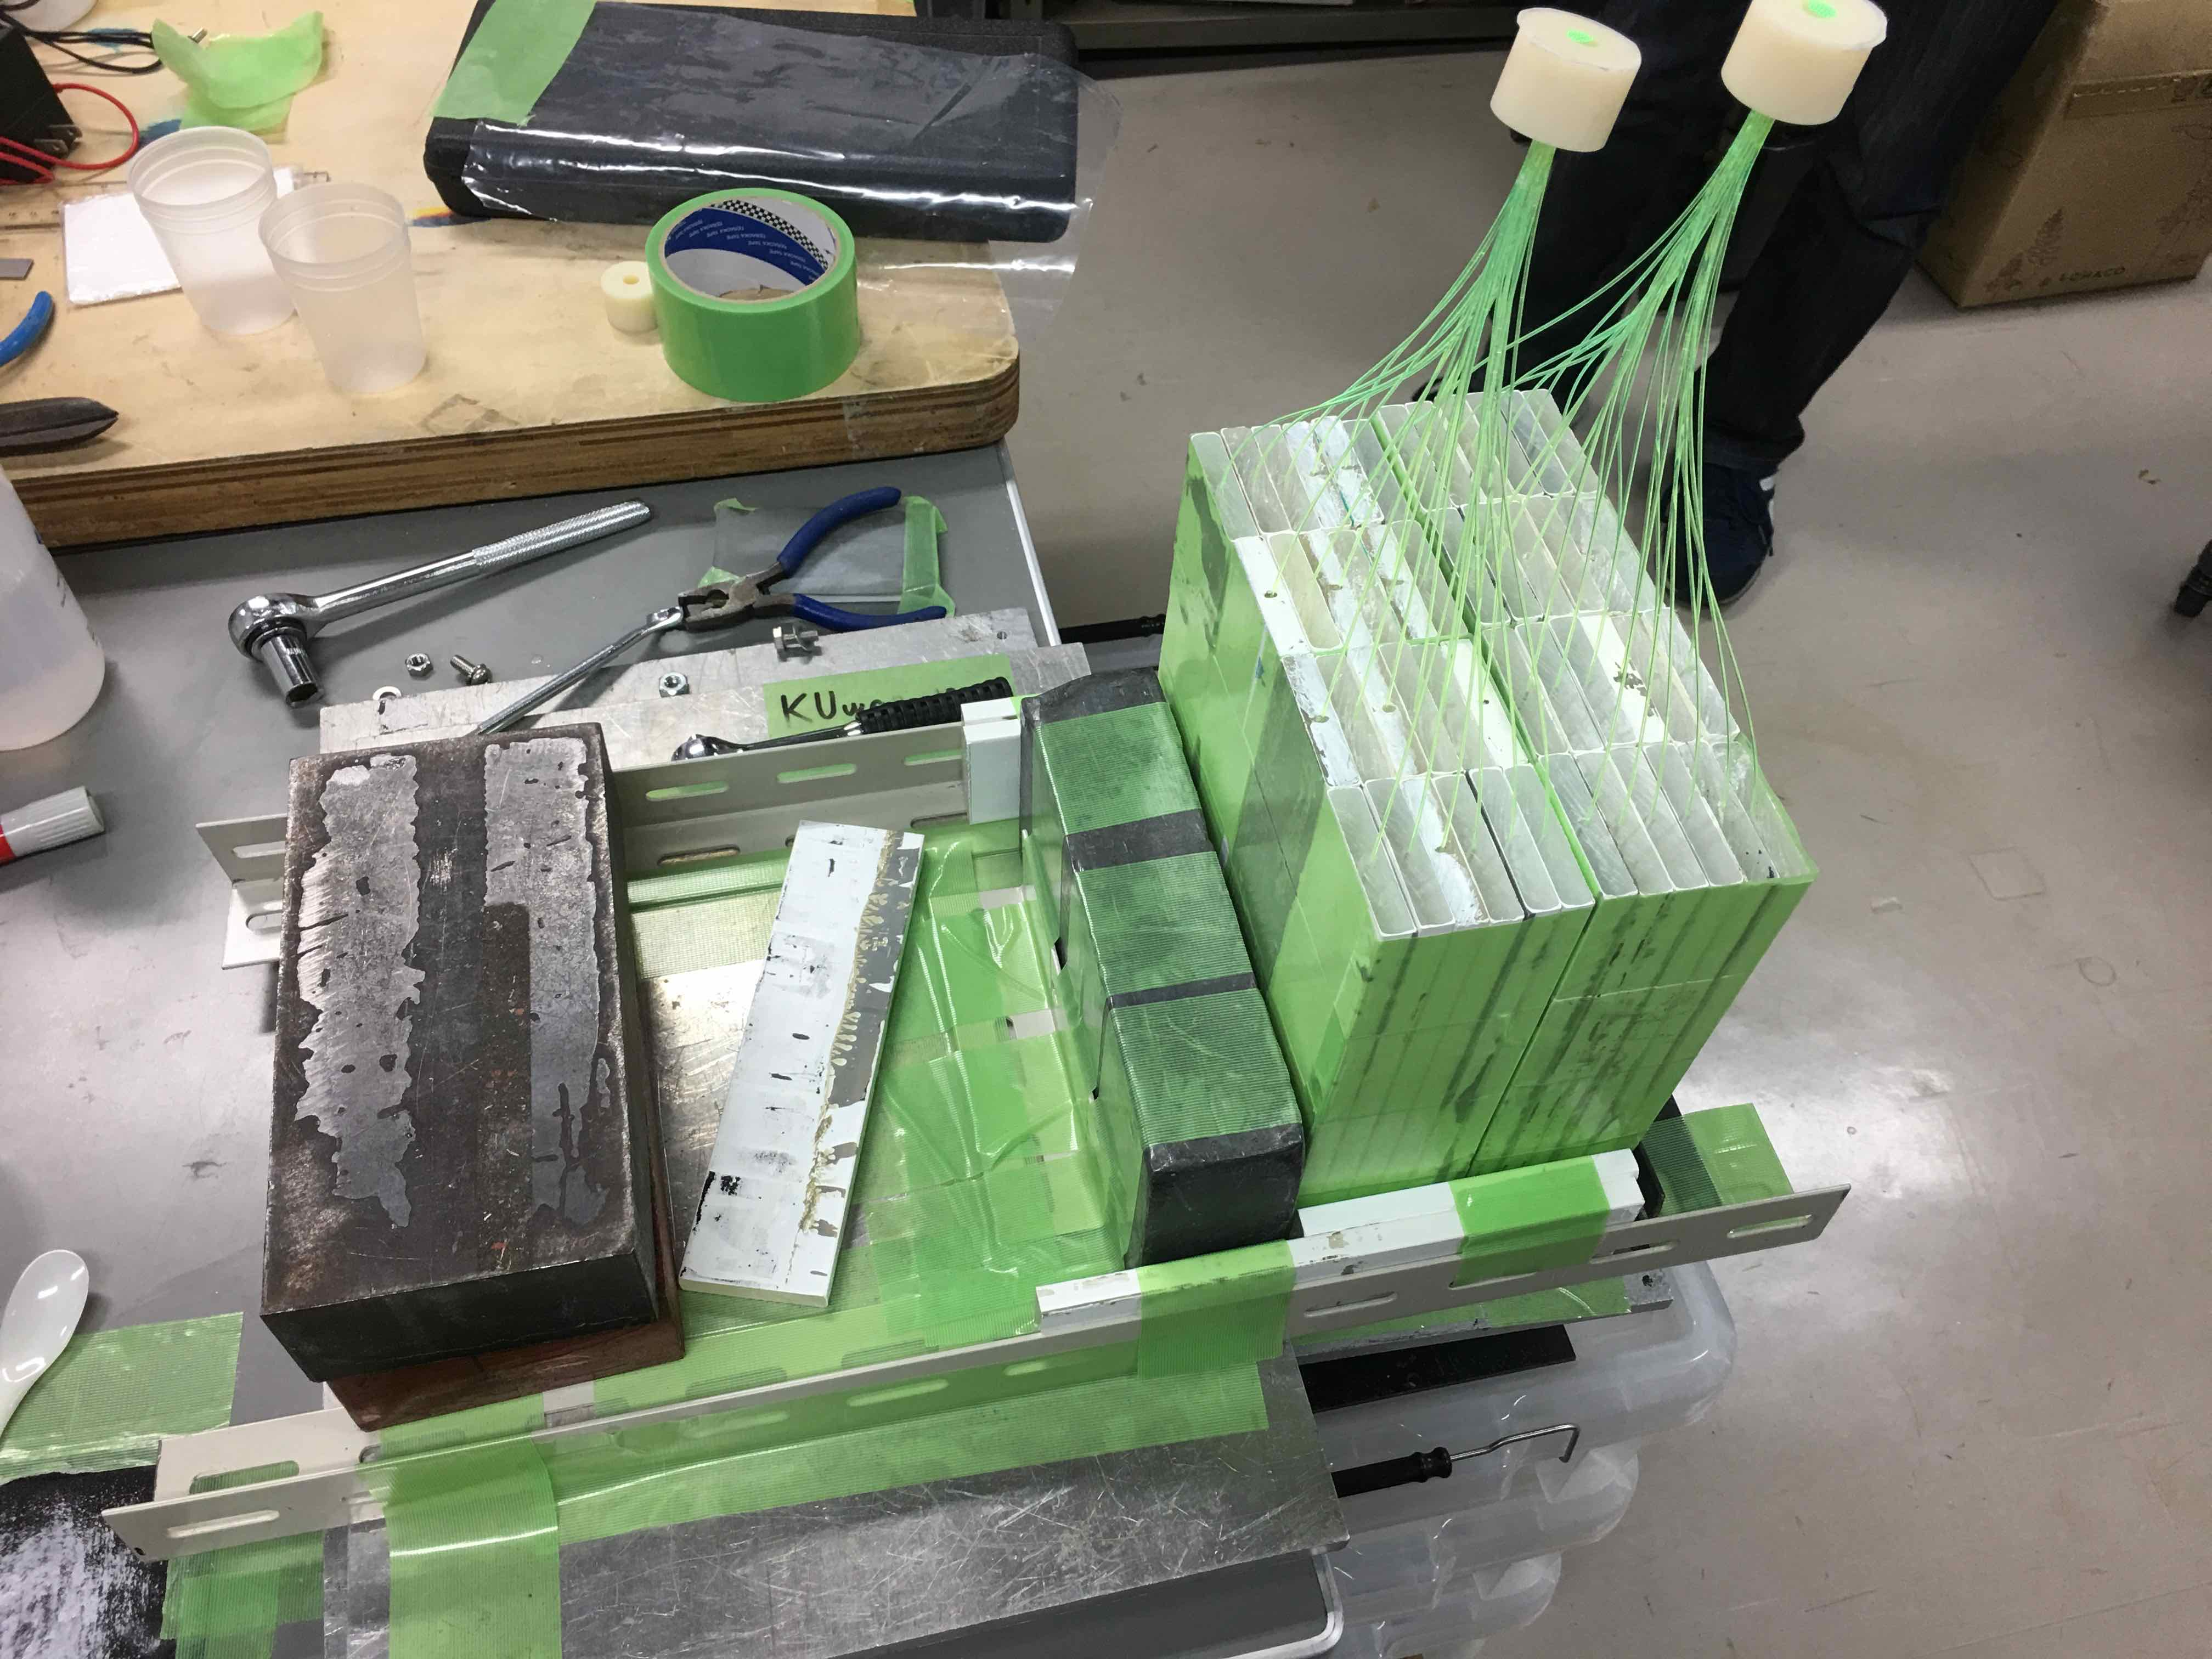
\includegraphics[width=0.5\textwidth]{figure/hayakawa/ps_kotei.jpg}
\caption{光ファイバーの固定の様子}
\end{figure}
\item PS に光ファイバーを貫通させ,もう片端も固定した
\item 光量を最大限確保するため,クッキーの端面を研磨した
\item クッキーの端面と PMT の境界に光学グリスを塗り接続した
\item 暗箱内に設置するための枠に収めた.枠とPMT の結合にはアルミU 型チャンネルを用いた
\begin{figure}[H]
\centering
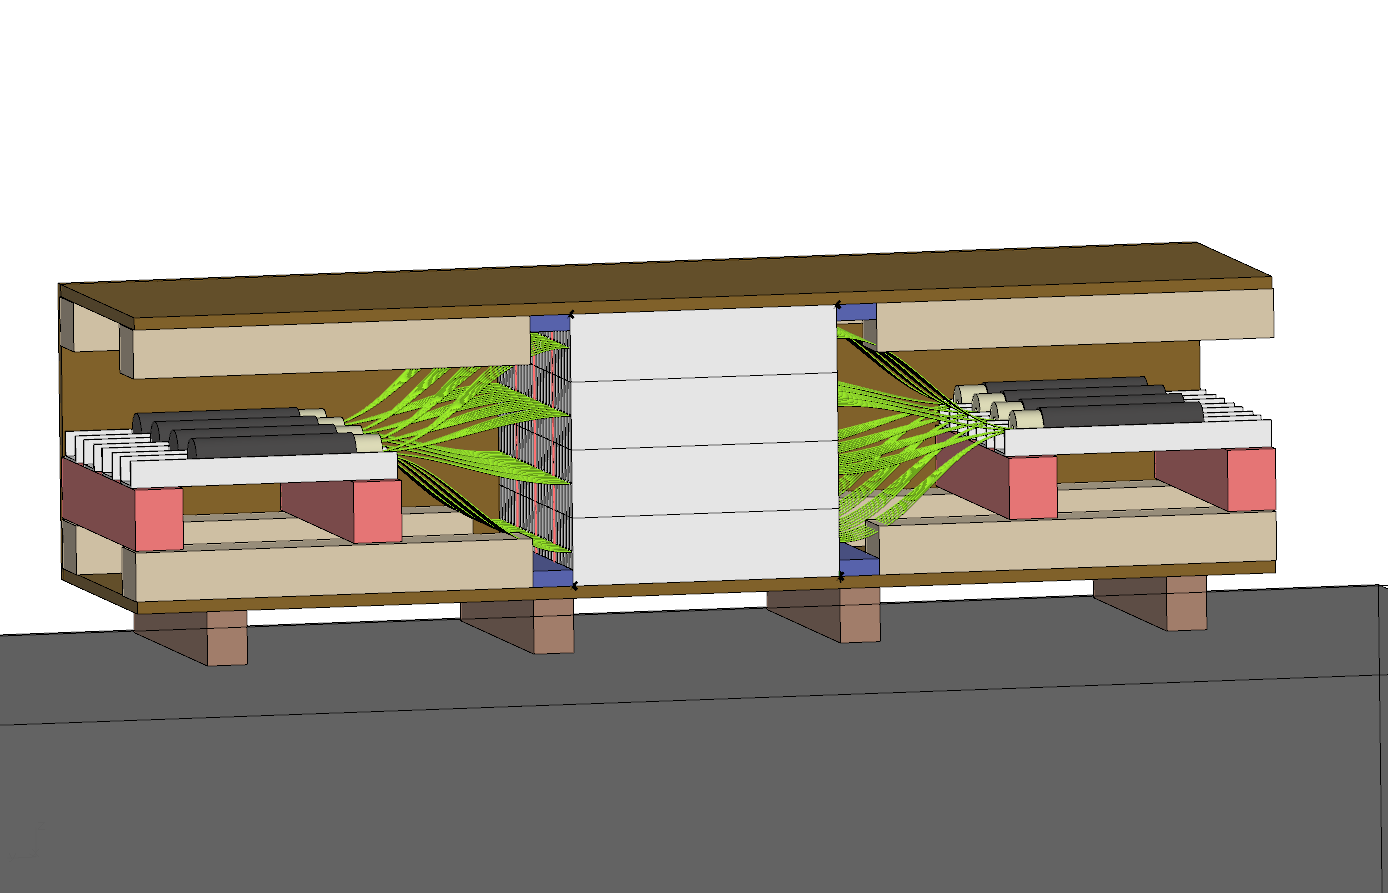
\includegraphics[width=0.6\textwidth]{figure/hayakawa/waku1.png}
\caption{暗箱に固定するための枠の設計}
\end{figure}
\item 暗箱内に設置し前方にコリメータを配置した
\end{itemize}

\begin{figure} [H]
\centering
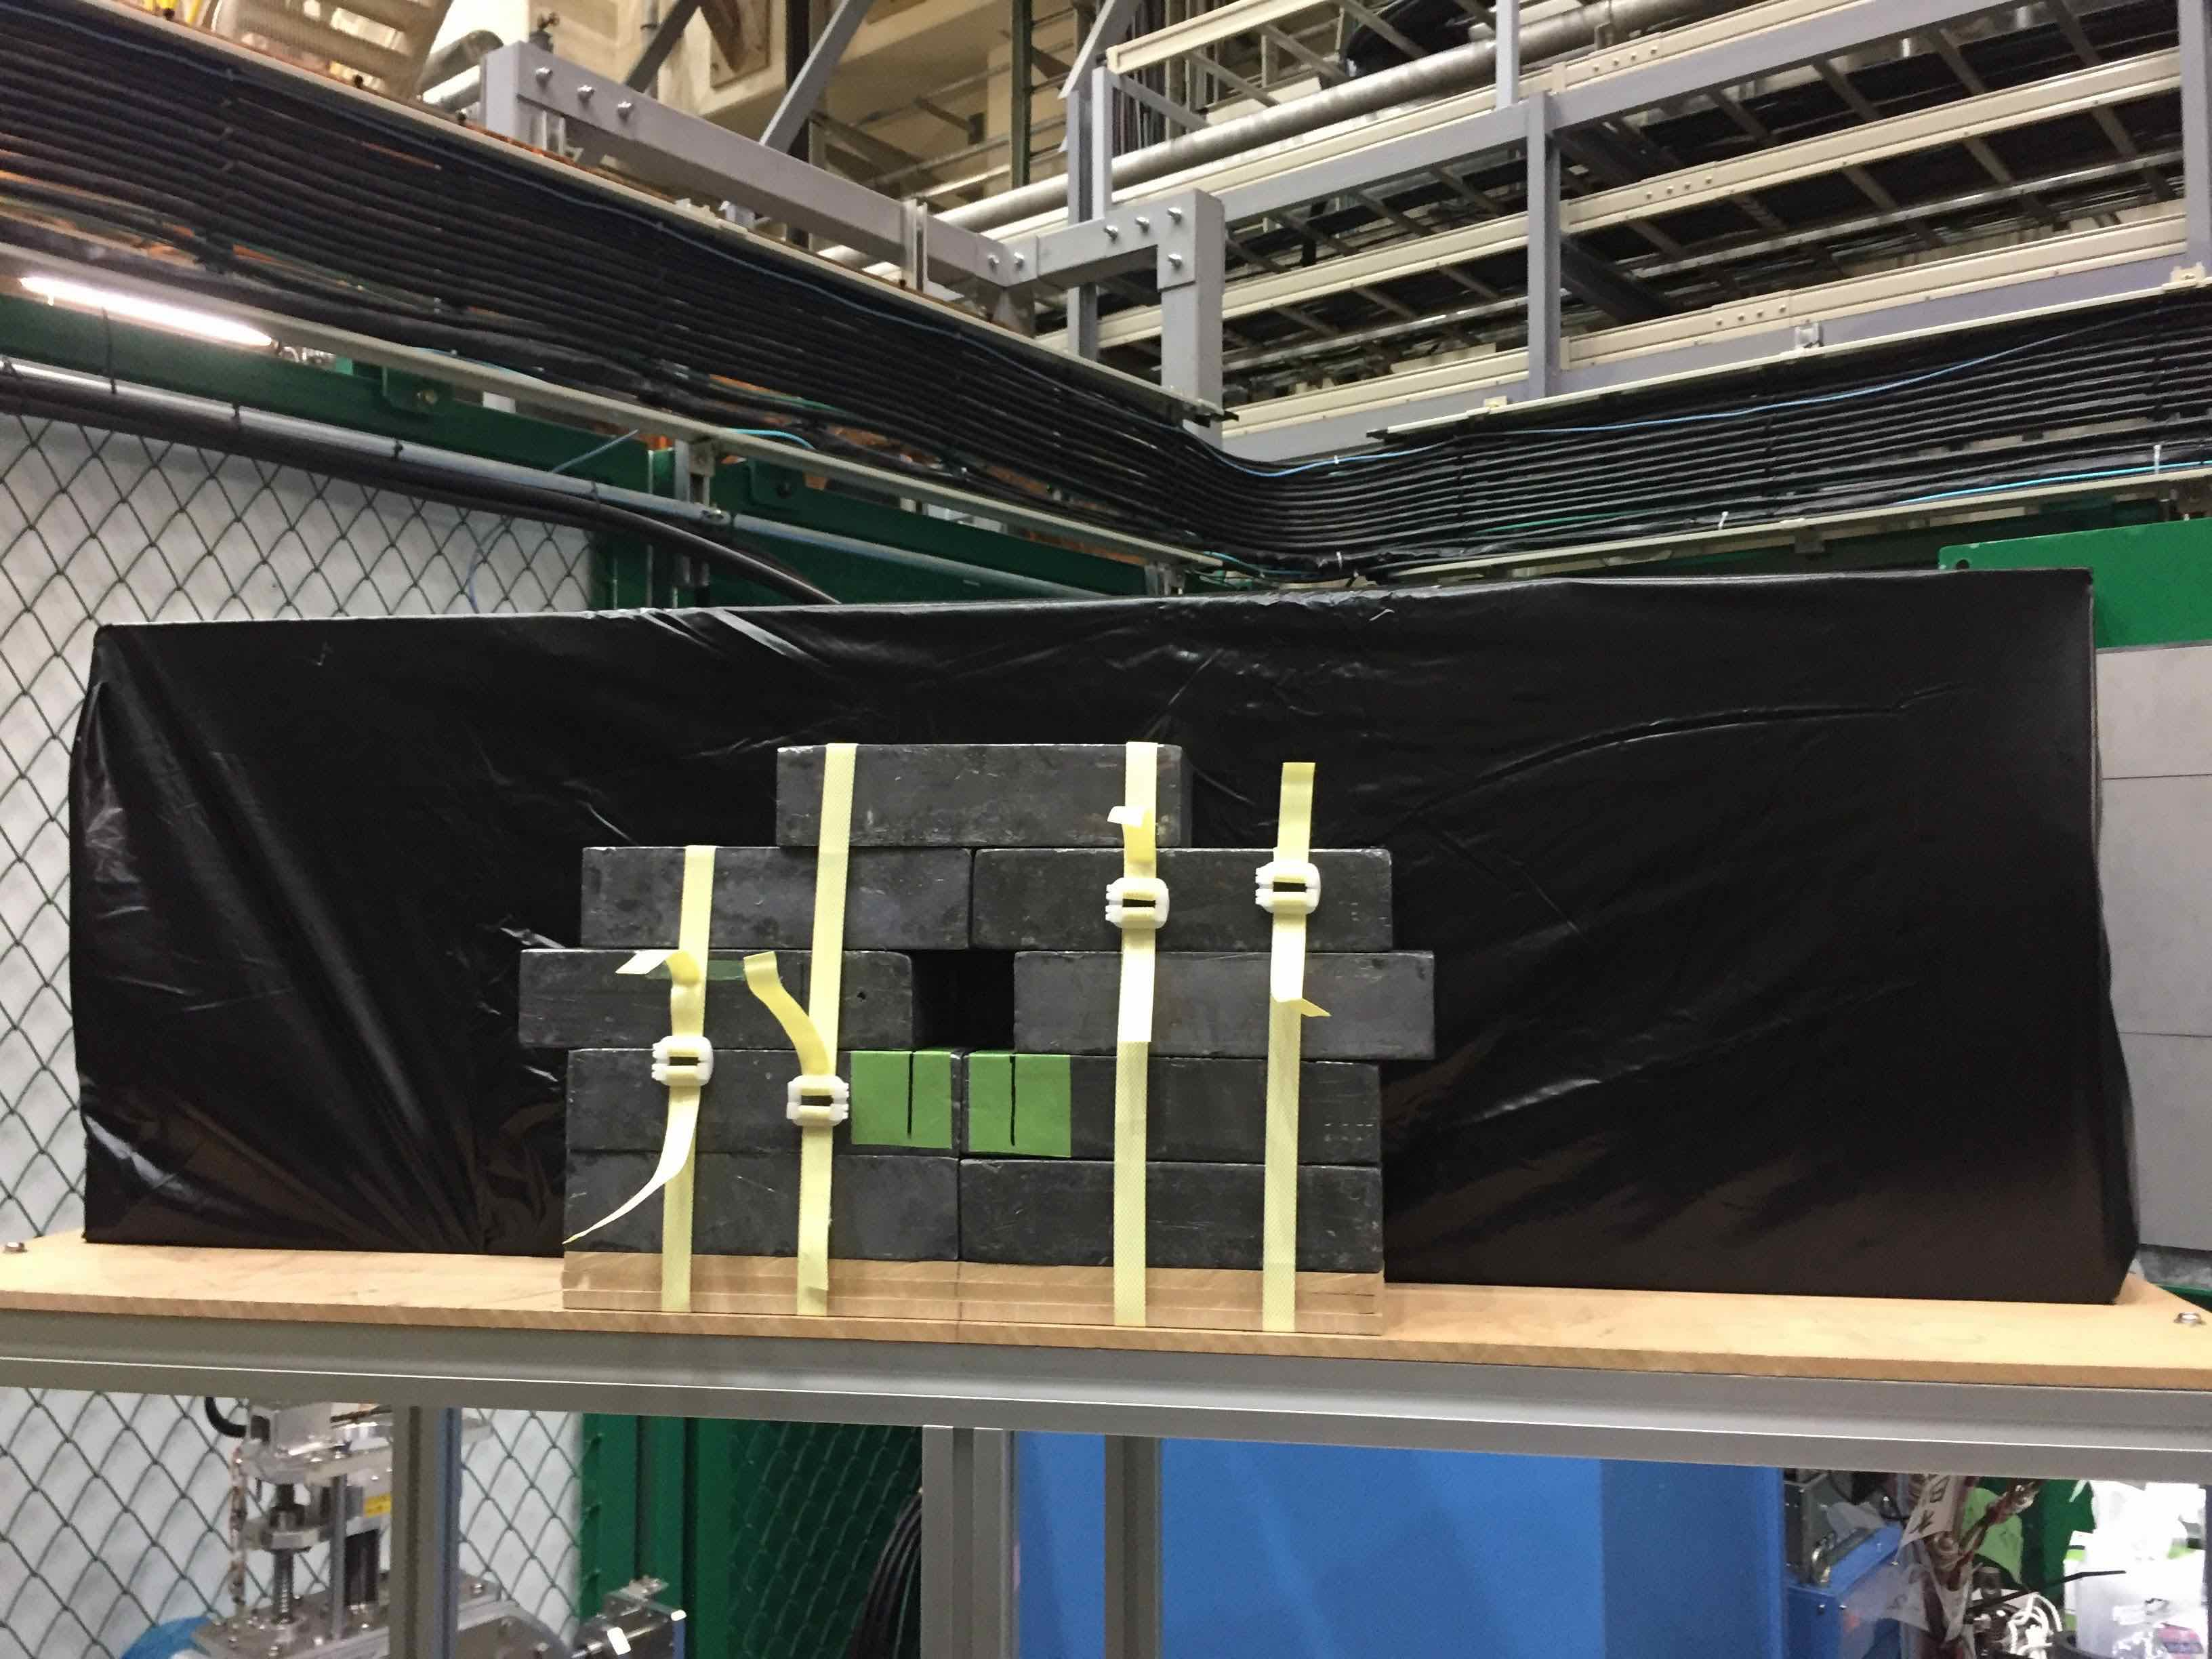
\includegraphics[width=0.6\textwidth]{figure/hayakawa/PS_real.jpg}
\caption{PS 検出器外観}
\end{figure}
\begin{figure}[H]
\centering
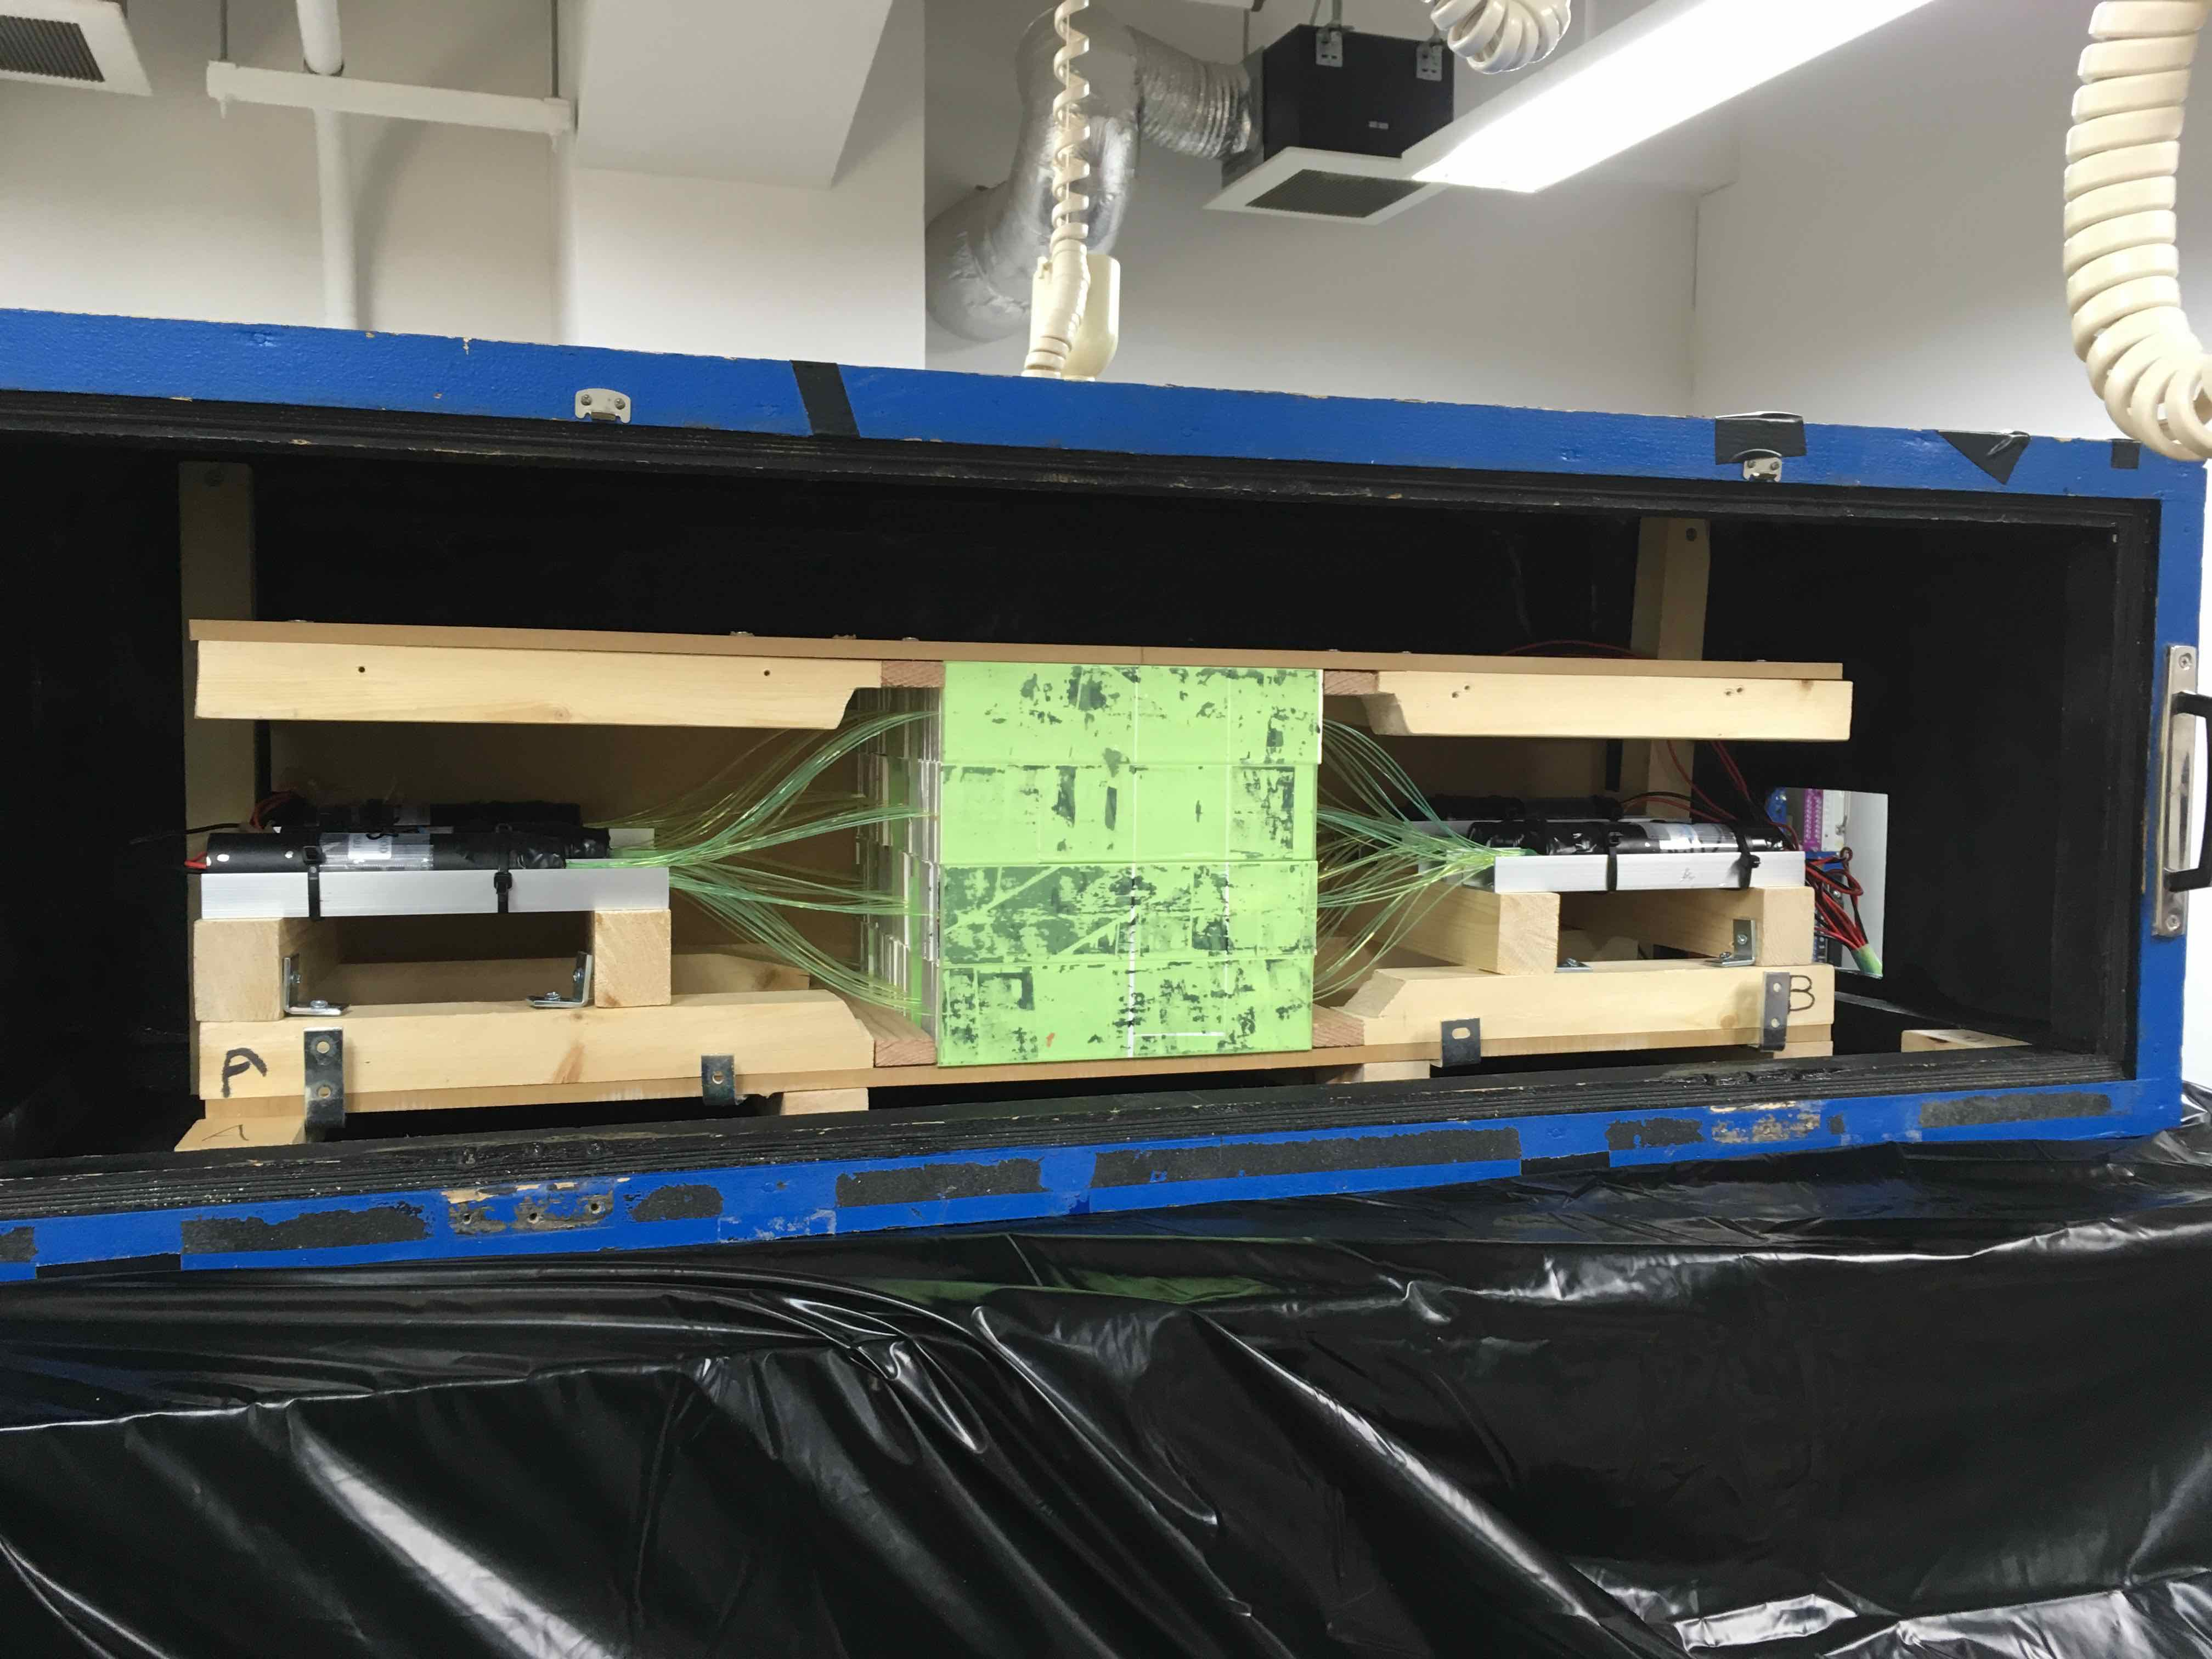
\includegraphics[width=0.7\textwidth]{figure/hayakawa/PS_in.jpg}
\caption{PS検出器内部}
\end{figure}

\subsubsection{NaI 検出器の製作}

$5.6~\mathrm{cm}\times 5.6~\mathrm{cm}\times 15~\mathrm{cm}$ のNaI (Tl) の結晶がPMT に接続されたもの(以下,NaI とよぶ)を$3\times 3$ 個並べ,検出器の前面中央の前には$4~\mathrm{cm} \times 4~\mathrm{cm}$ のプラスチックシンチレータで作ったトリガー用カウンターを設置した.
\begin{figure}
\begin{tabular}{cc}
\begin{minipage}{0.5\hsize}
\centering
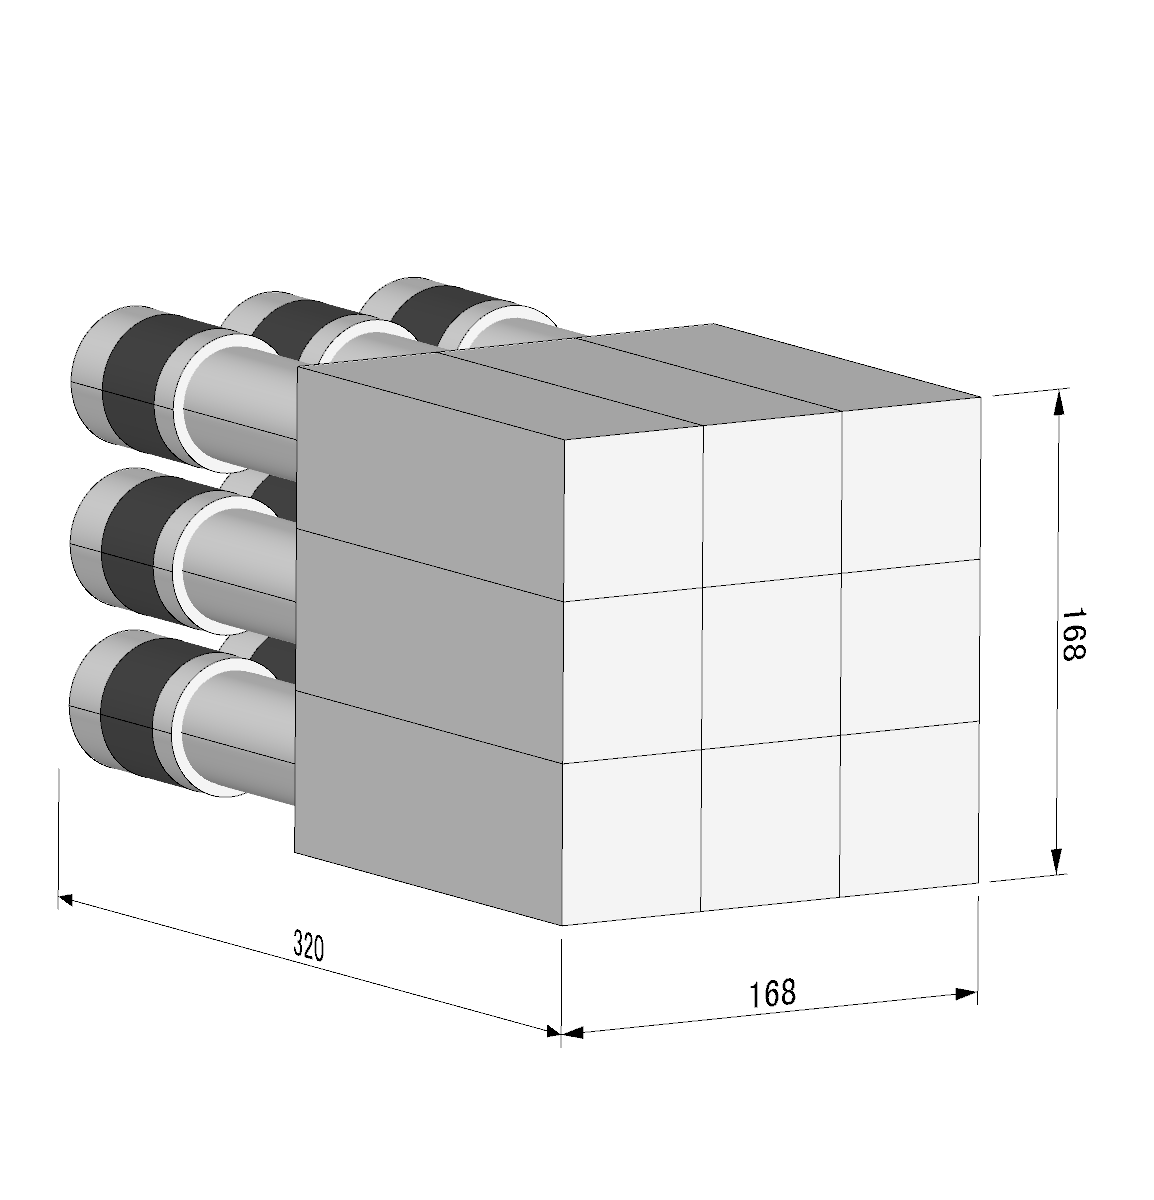
\includegraphics[width=0.8\textwidth]{figure/hayakawa/p6.png}
\caption{NaI 寸法 (mm)}
\end{minipage}
\begin{minipage}{0.5\hsize}
\centering
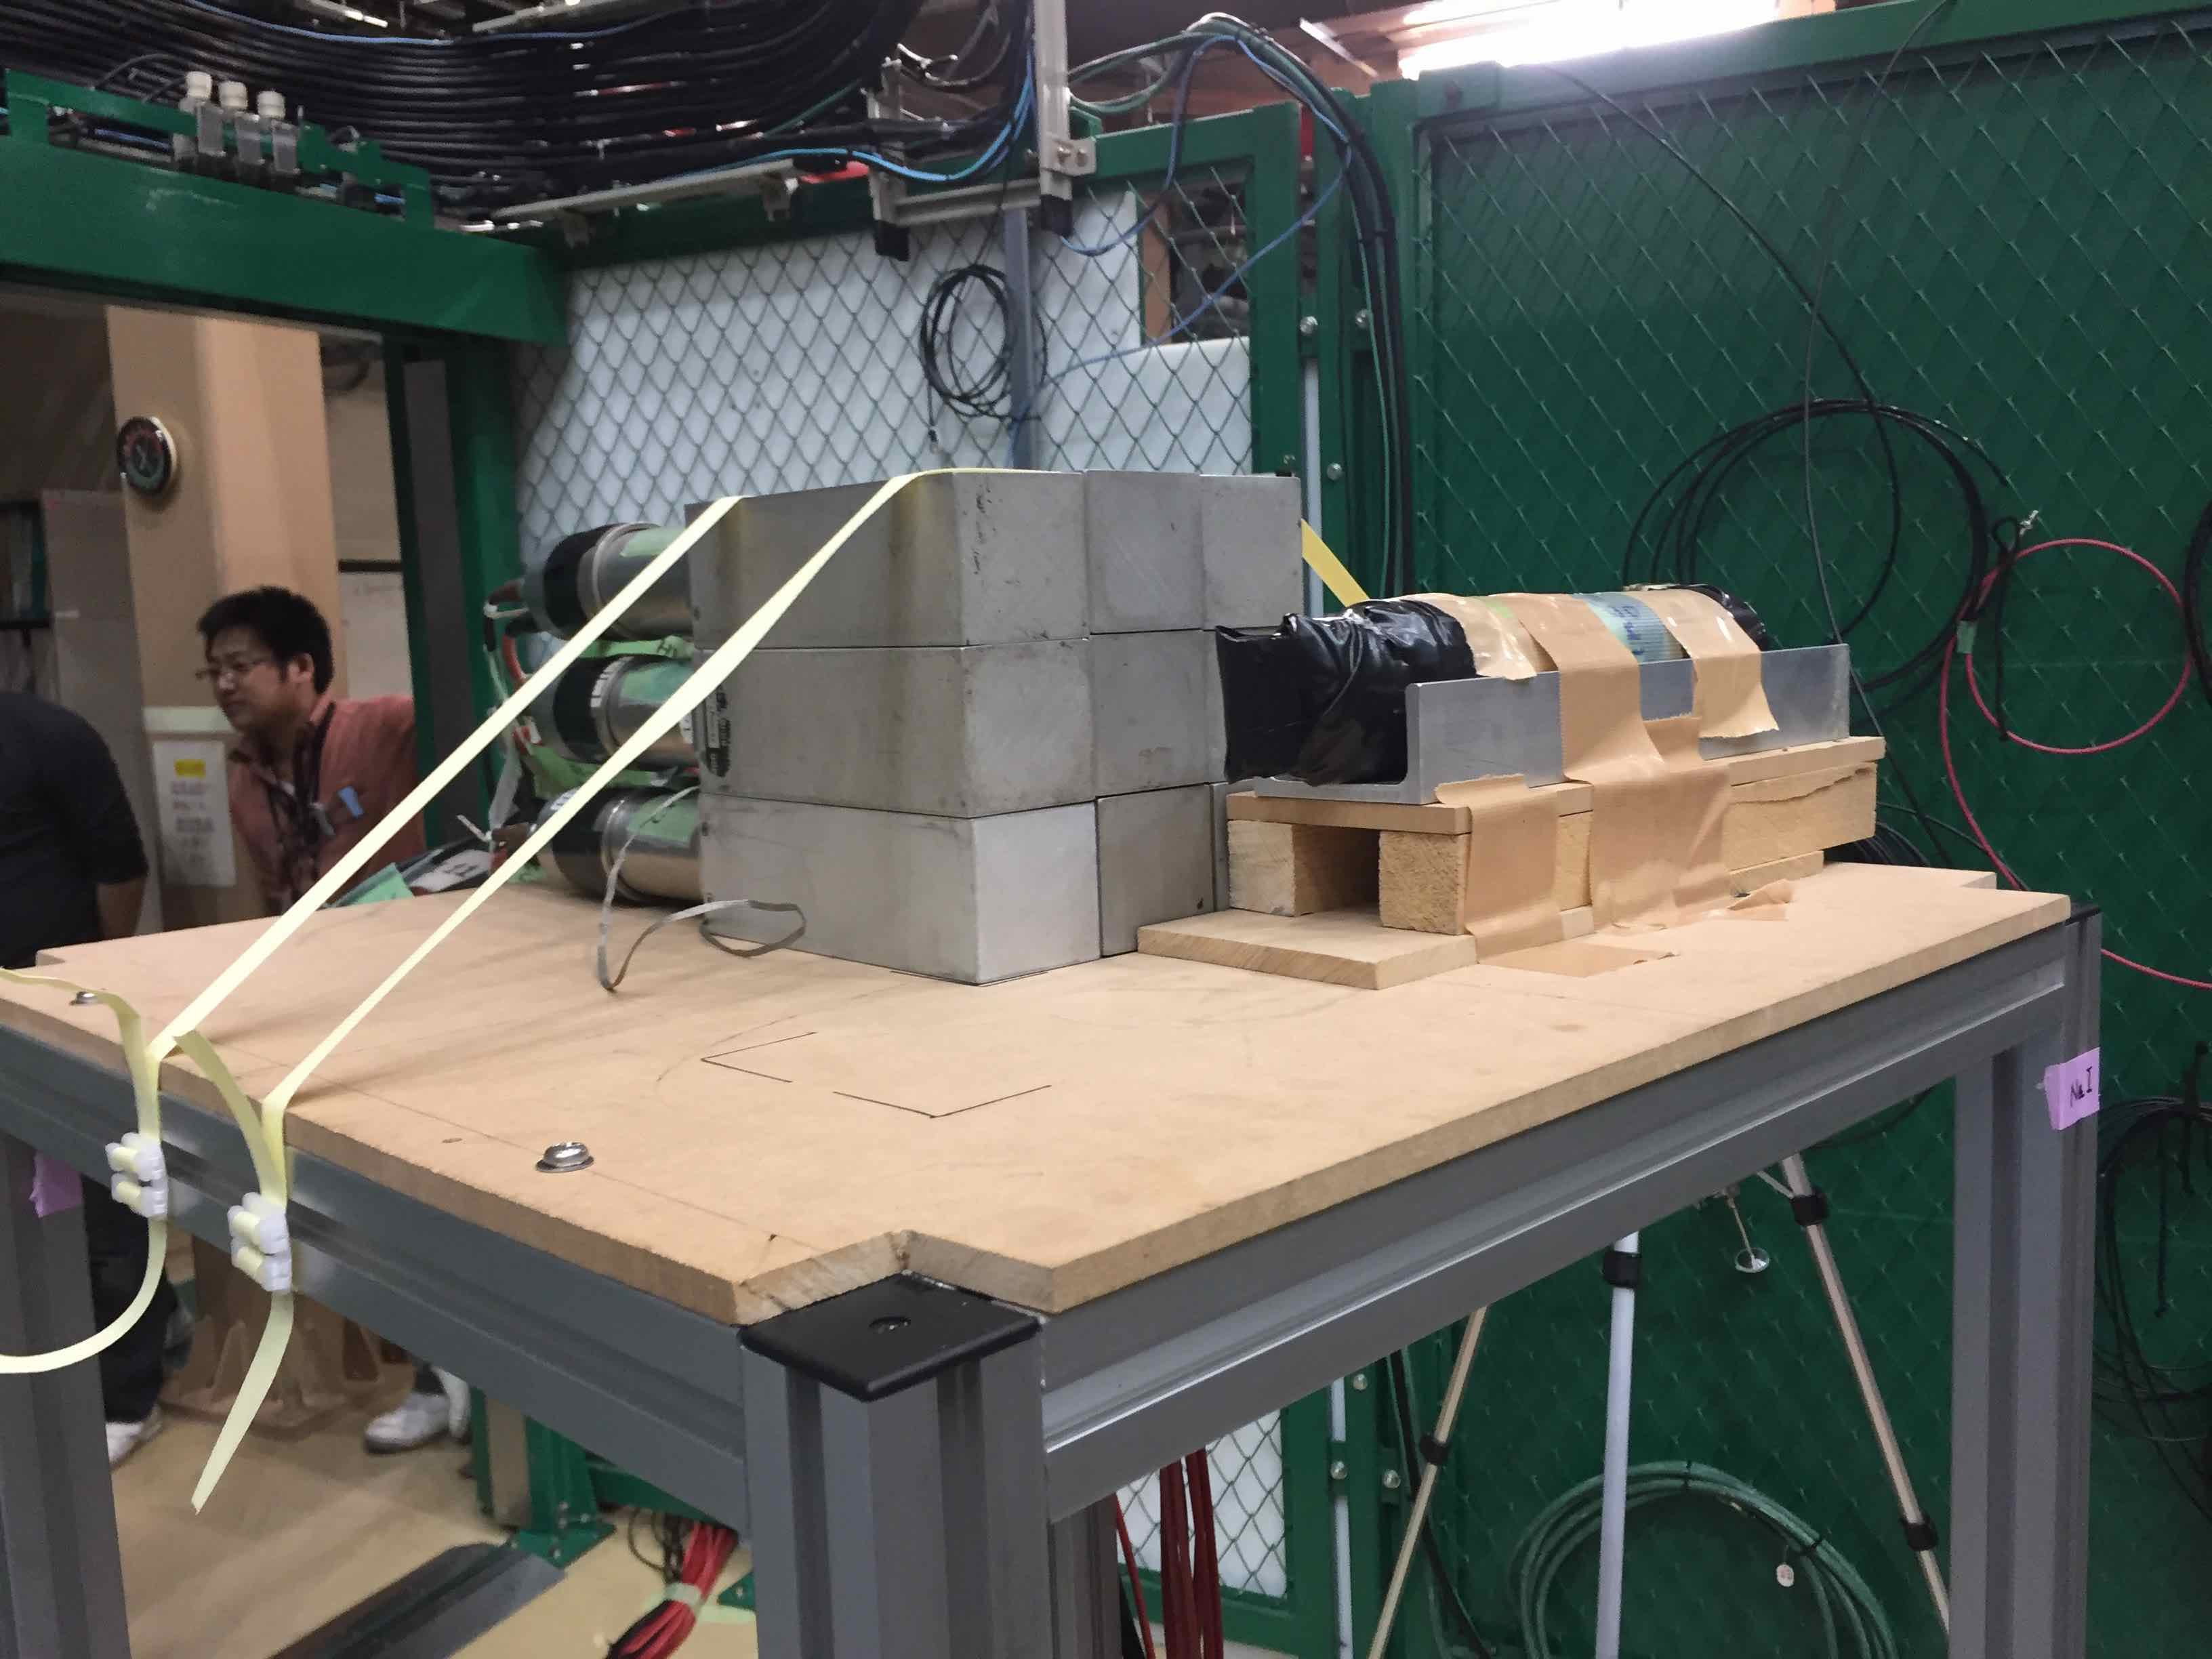
\includegraphics[width=0.8\textwidth]{figure/hayakawa/NaI_real.jpg}
\caption{NaI 外観}
\end{minipage}
\end{tabular}
\end{figure}

\subsection{架台の製作}

ビームの出る高さが地表から$1565~\mathrm{mm}$ なので,検出器を置くためにはその高さに対応した架台が必要であった.そこでアルミフレームの一種であるレコフレームを使用して架台を作成した.アジャスタ付きキャスタを用いることによって高さは微調整可能なように設計した.現場ではレーザーを用いて水平および垂直方向の位置調整を行った.

\begin{figure}[H]
\begin{tabular}{cc}
\begin{minipage}{0.5\hsize}
\centering
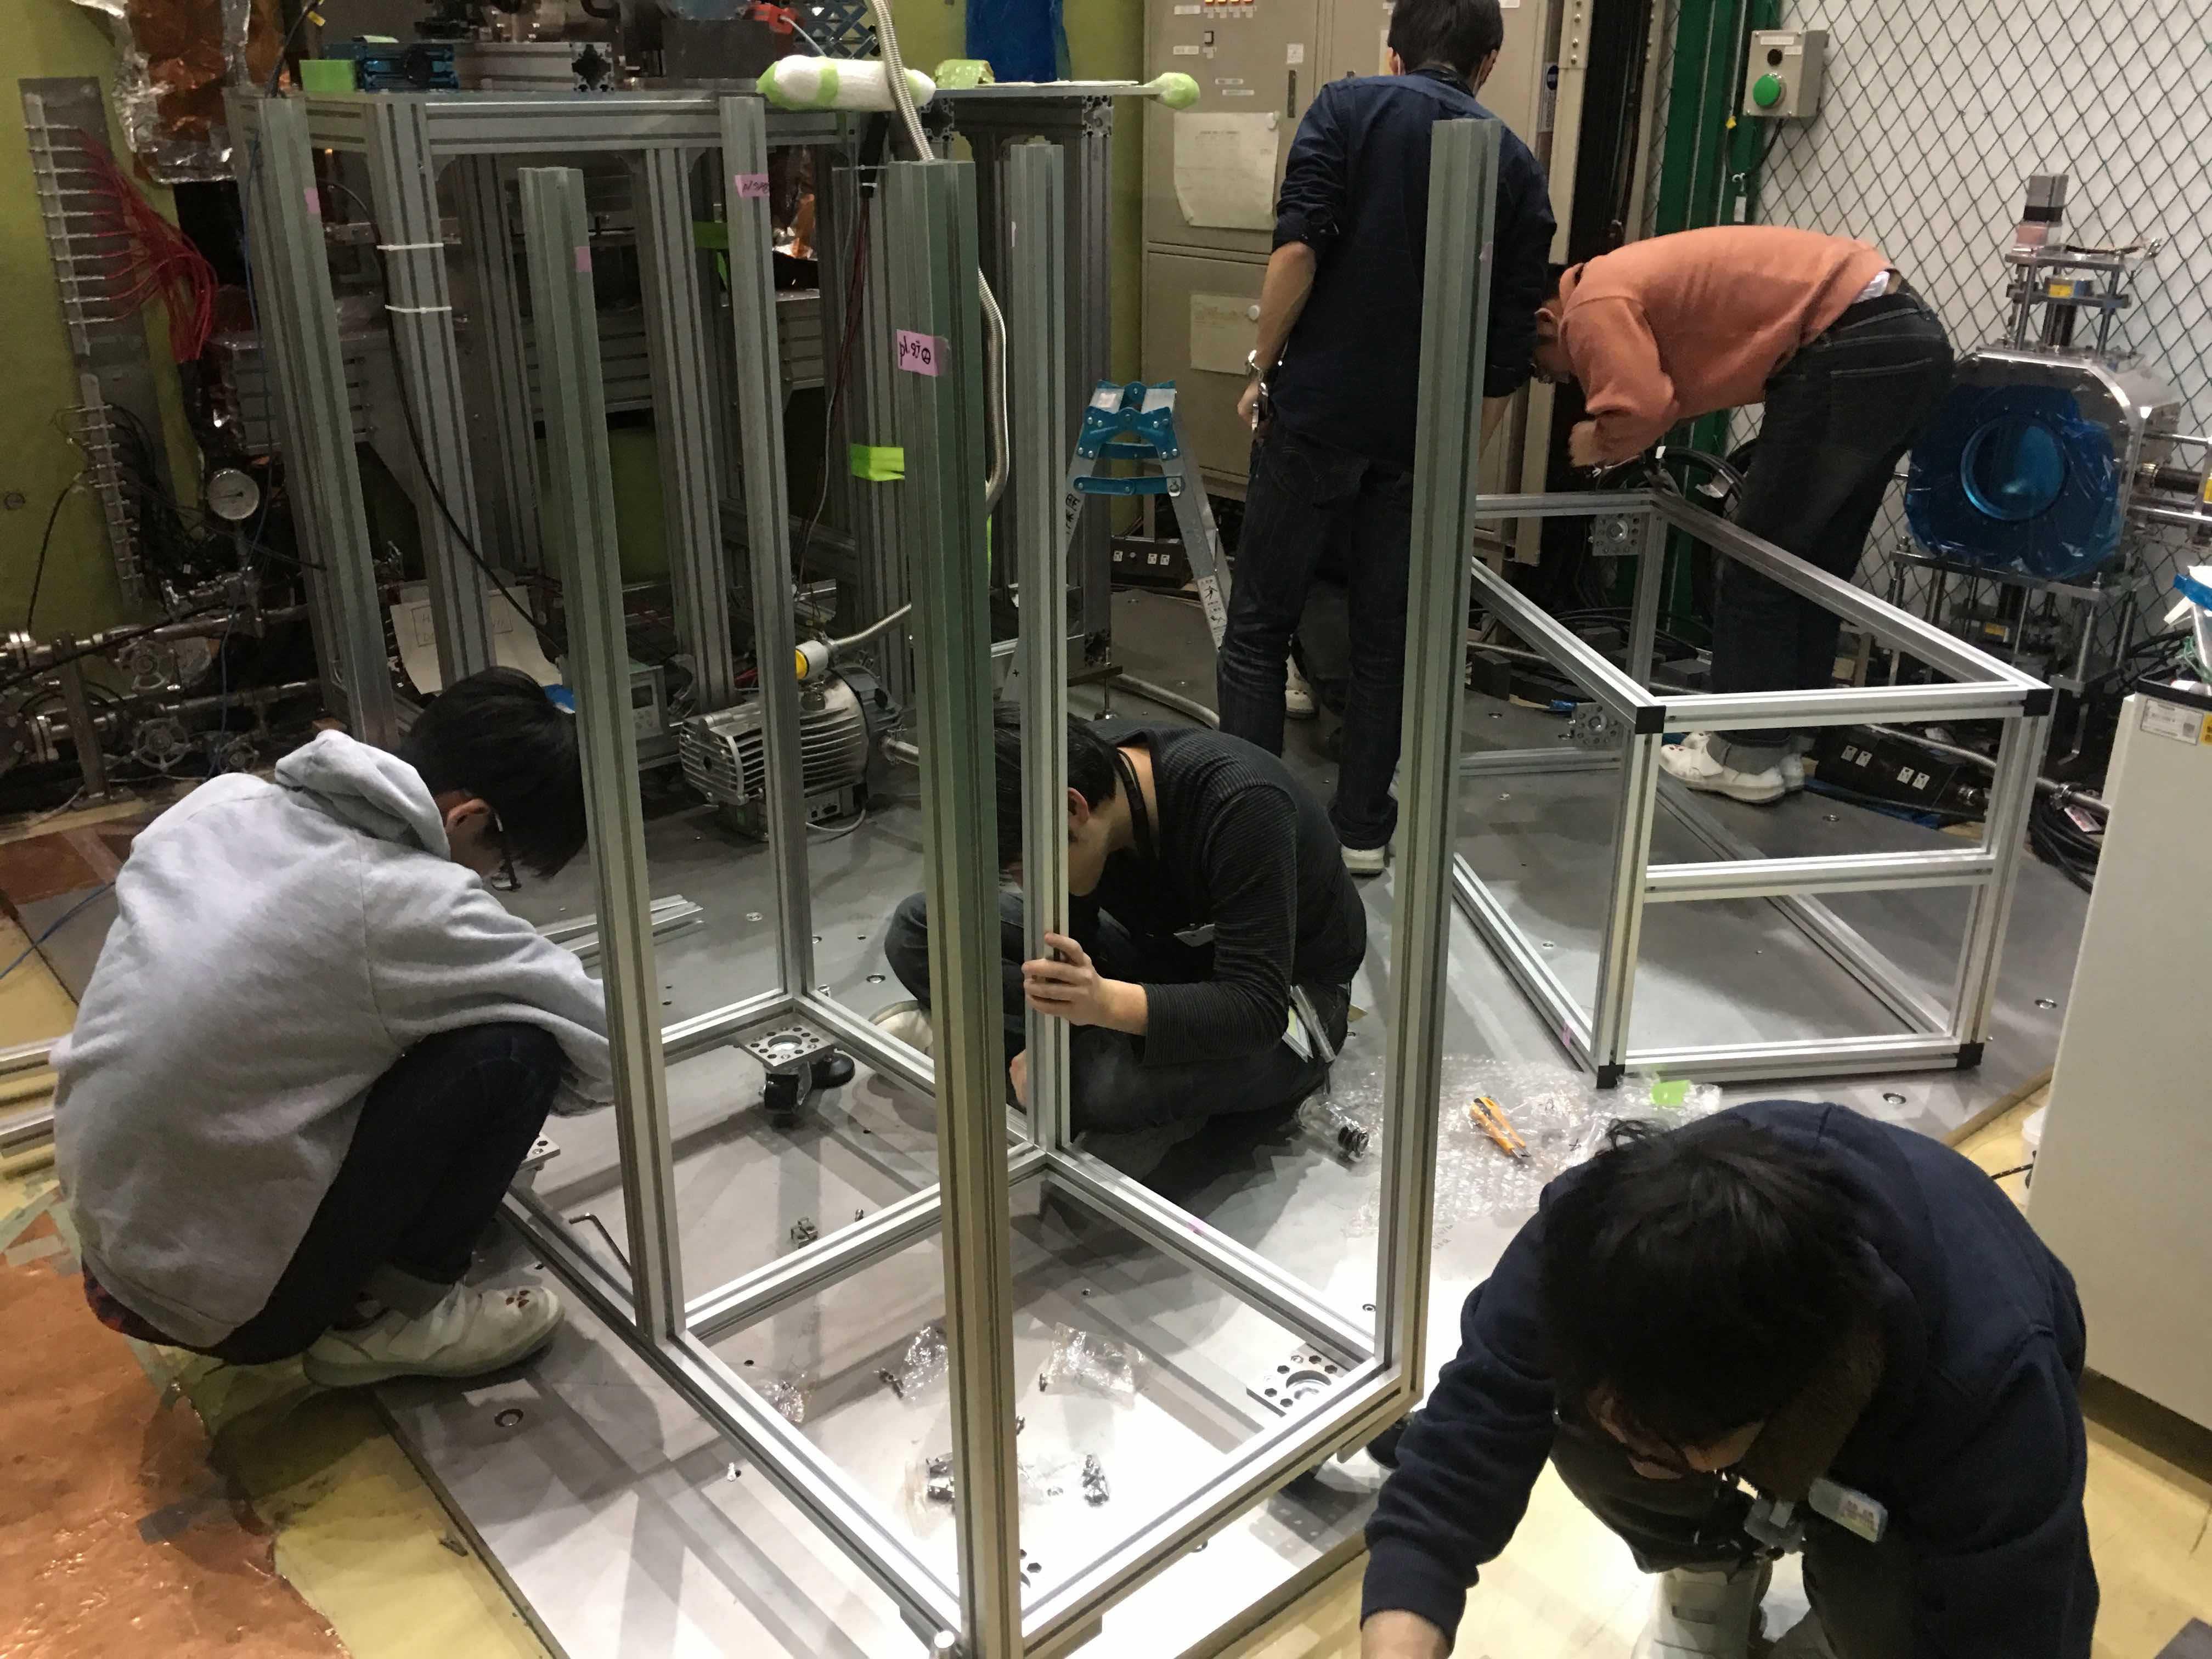
\includegraphics[width=0.9\textwidth]{figure/hayakawa/kadai_setup.jpg}
\caption{架台の組み立て}
\end{minipage}
\begin{minipage}{0.5\hsize}
\centering
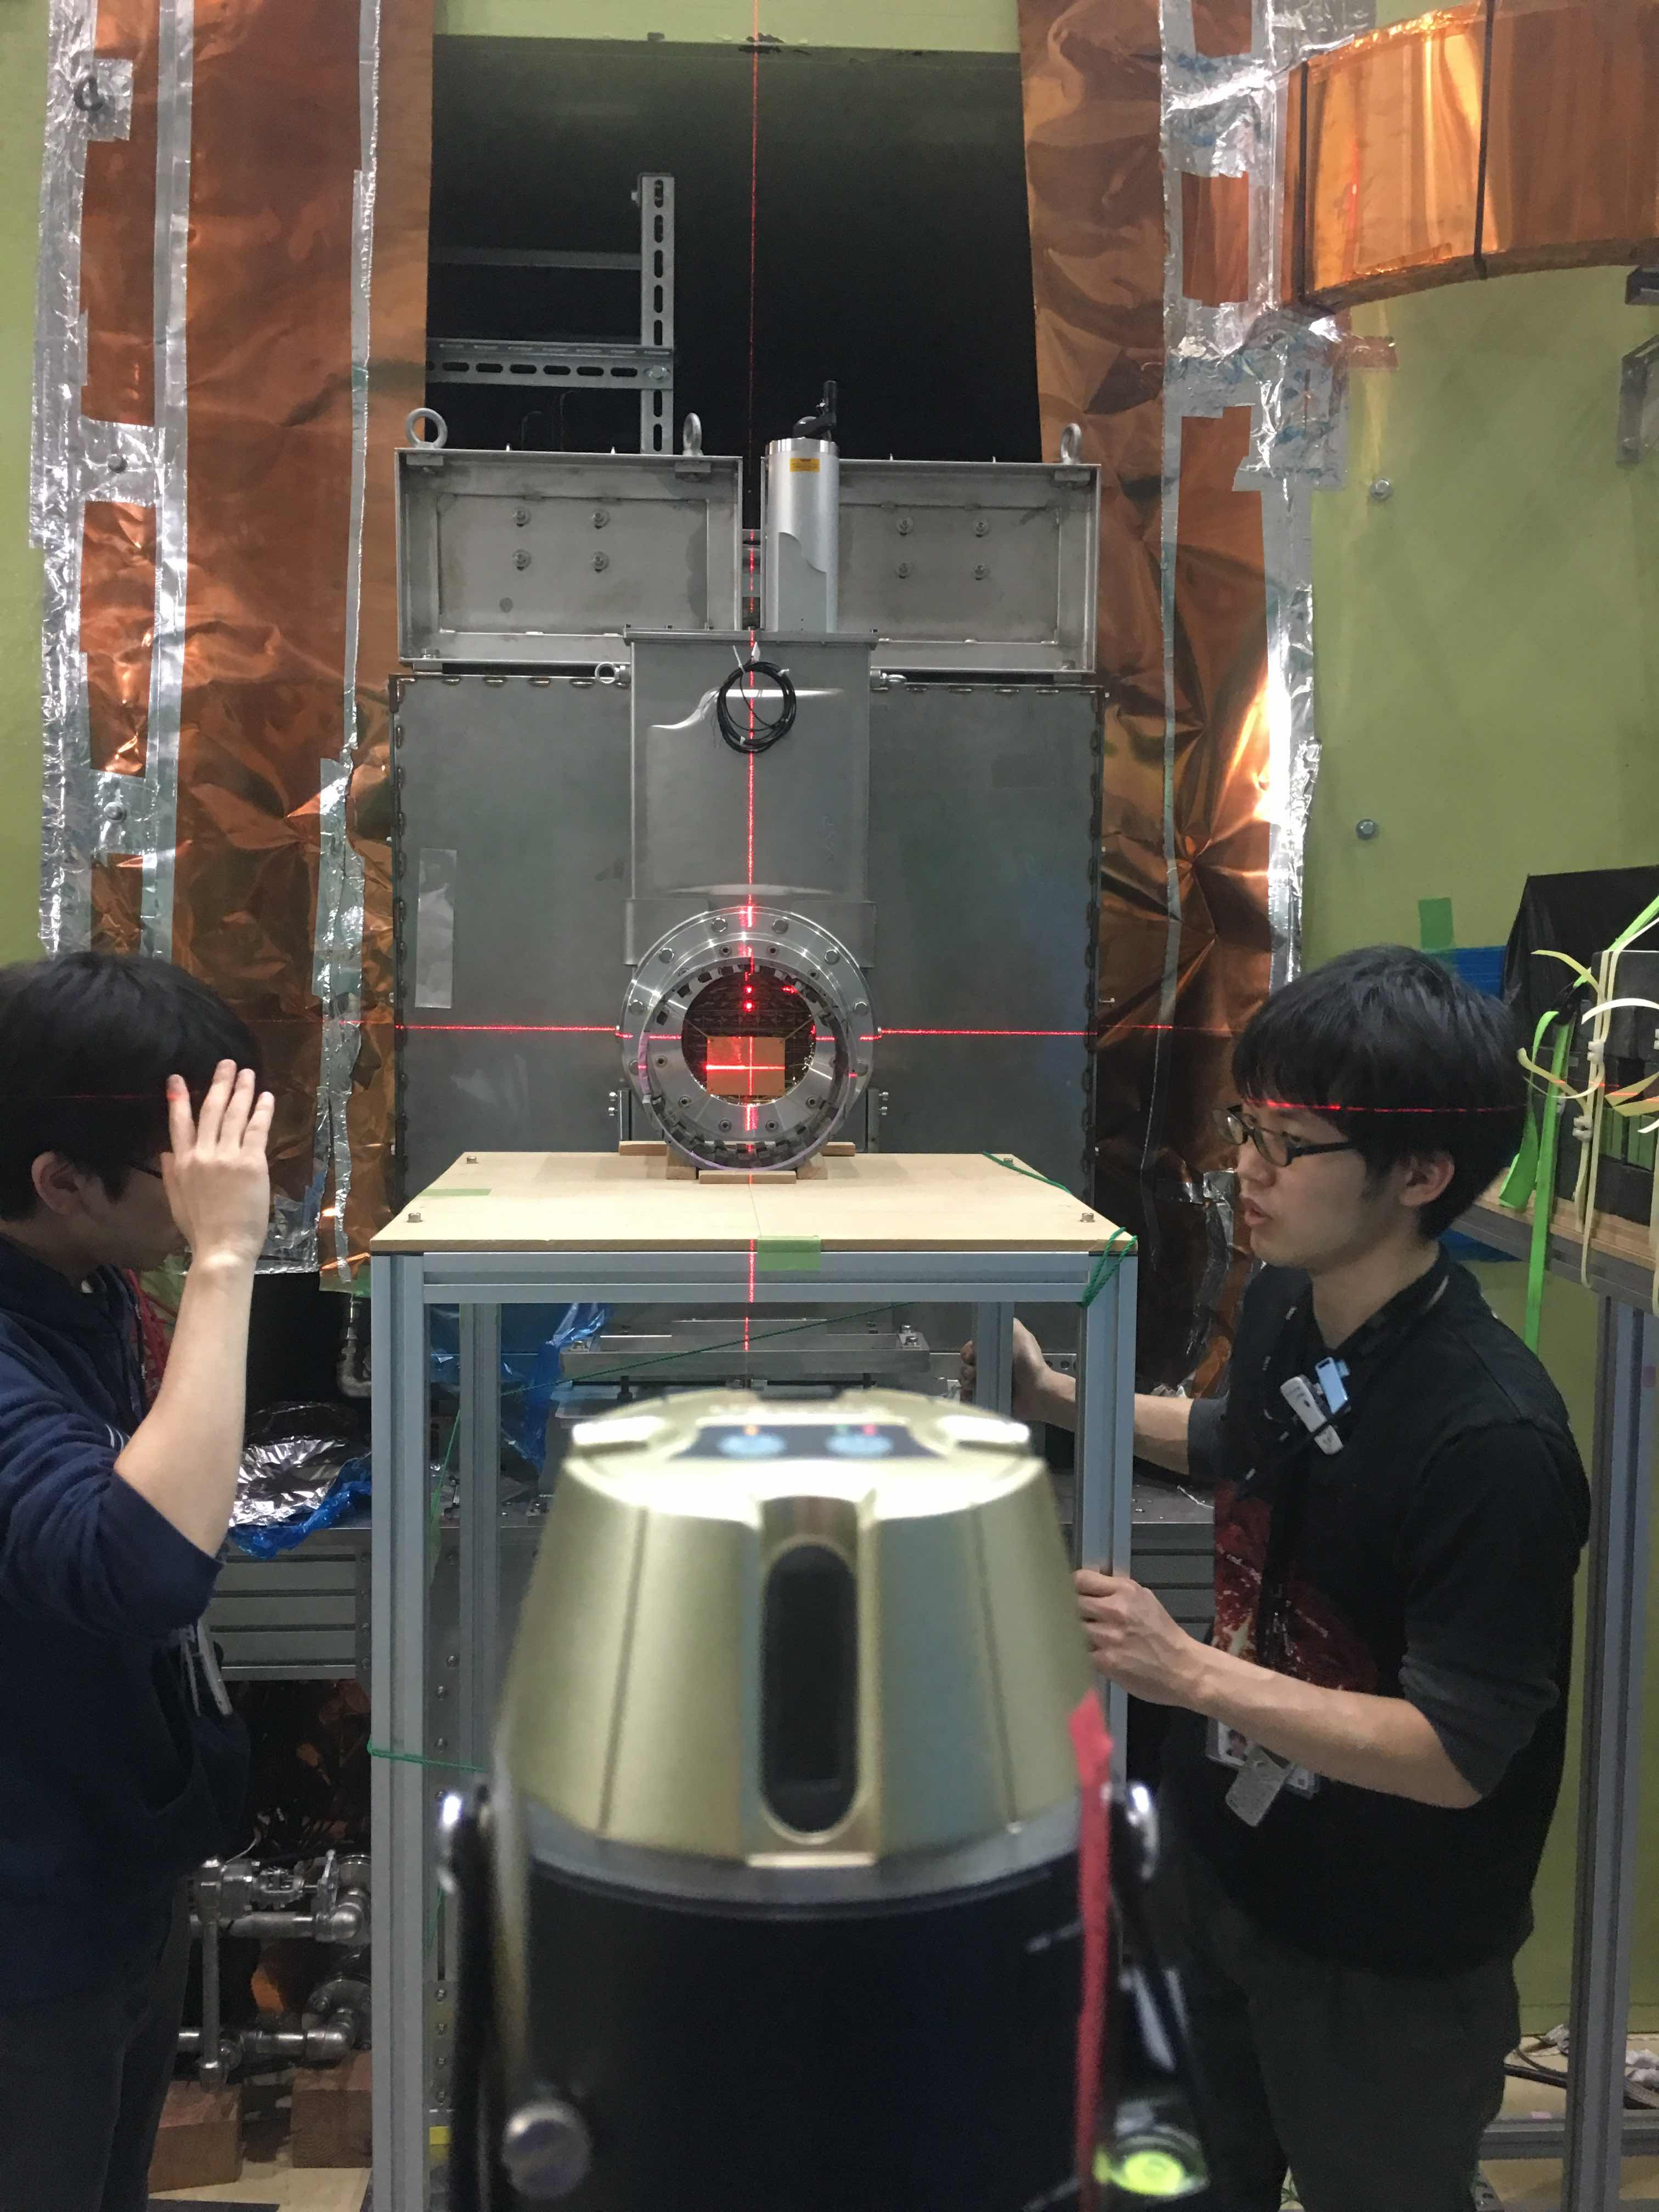
\includegraphics[width=0.9\textwidth]{figure/hayakawa/laser1.jpg}
\caption{レーザーを用いた位置調整}
\end{minipage}
\end{tabular}
 \end{figure}
  
\begin{table}[H]
\caption{3種類の架台の外寸}
\label{tab:kadai}
\centering
\begin{tabular}{|c|c|}\hline
{} &  W $\times$ D $\times$ H (mm)\\ \hline
PS 検出器架台 &  1200 $\times$ 600 $\times$ 1283\\ \hline
NaI 検出器架台 & 600 $\times$ 600 $\times$ 1358 \\ \hline
ターゲット架台 & 600 $\times$ 600 $\times$ 1331 \\ \hline
\end{tabular}
\end{table}

\subsection{Waveform Digitizer}

データ測定については波形をそのまま記録することができるWaveform Digitizer (以下,WFD とよぶ) をPS 検出器およびNaI 検出器用にそれぞれ利用した.測定開始の外部トリガには,加速器ライン側のビームの発射信号を遅延させて陽電子の崩壊の検出のスタートよりわずか手前になるように調整して入力している.

\subsubsection{WFD (CAEN Waveform Digitizer V1721)}
\begin{itemize}
\item 8~channel 8~bit 500~MS/s Digitizer
\item 時間分解能が良いので,主に崩壊寿命測定用のPS の信号に用いた
\end{itemize}
\begin{figure}[H]
\begin{tabular}{cc}
\begin{minipage}{0.5\hsize}
\centering
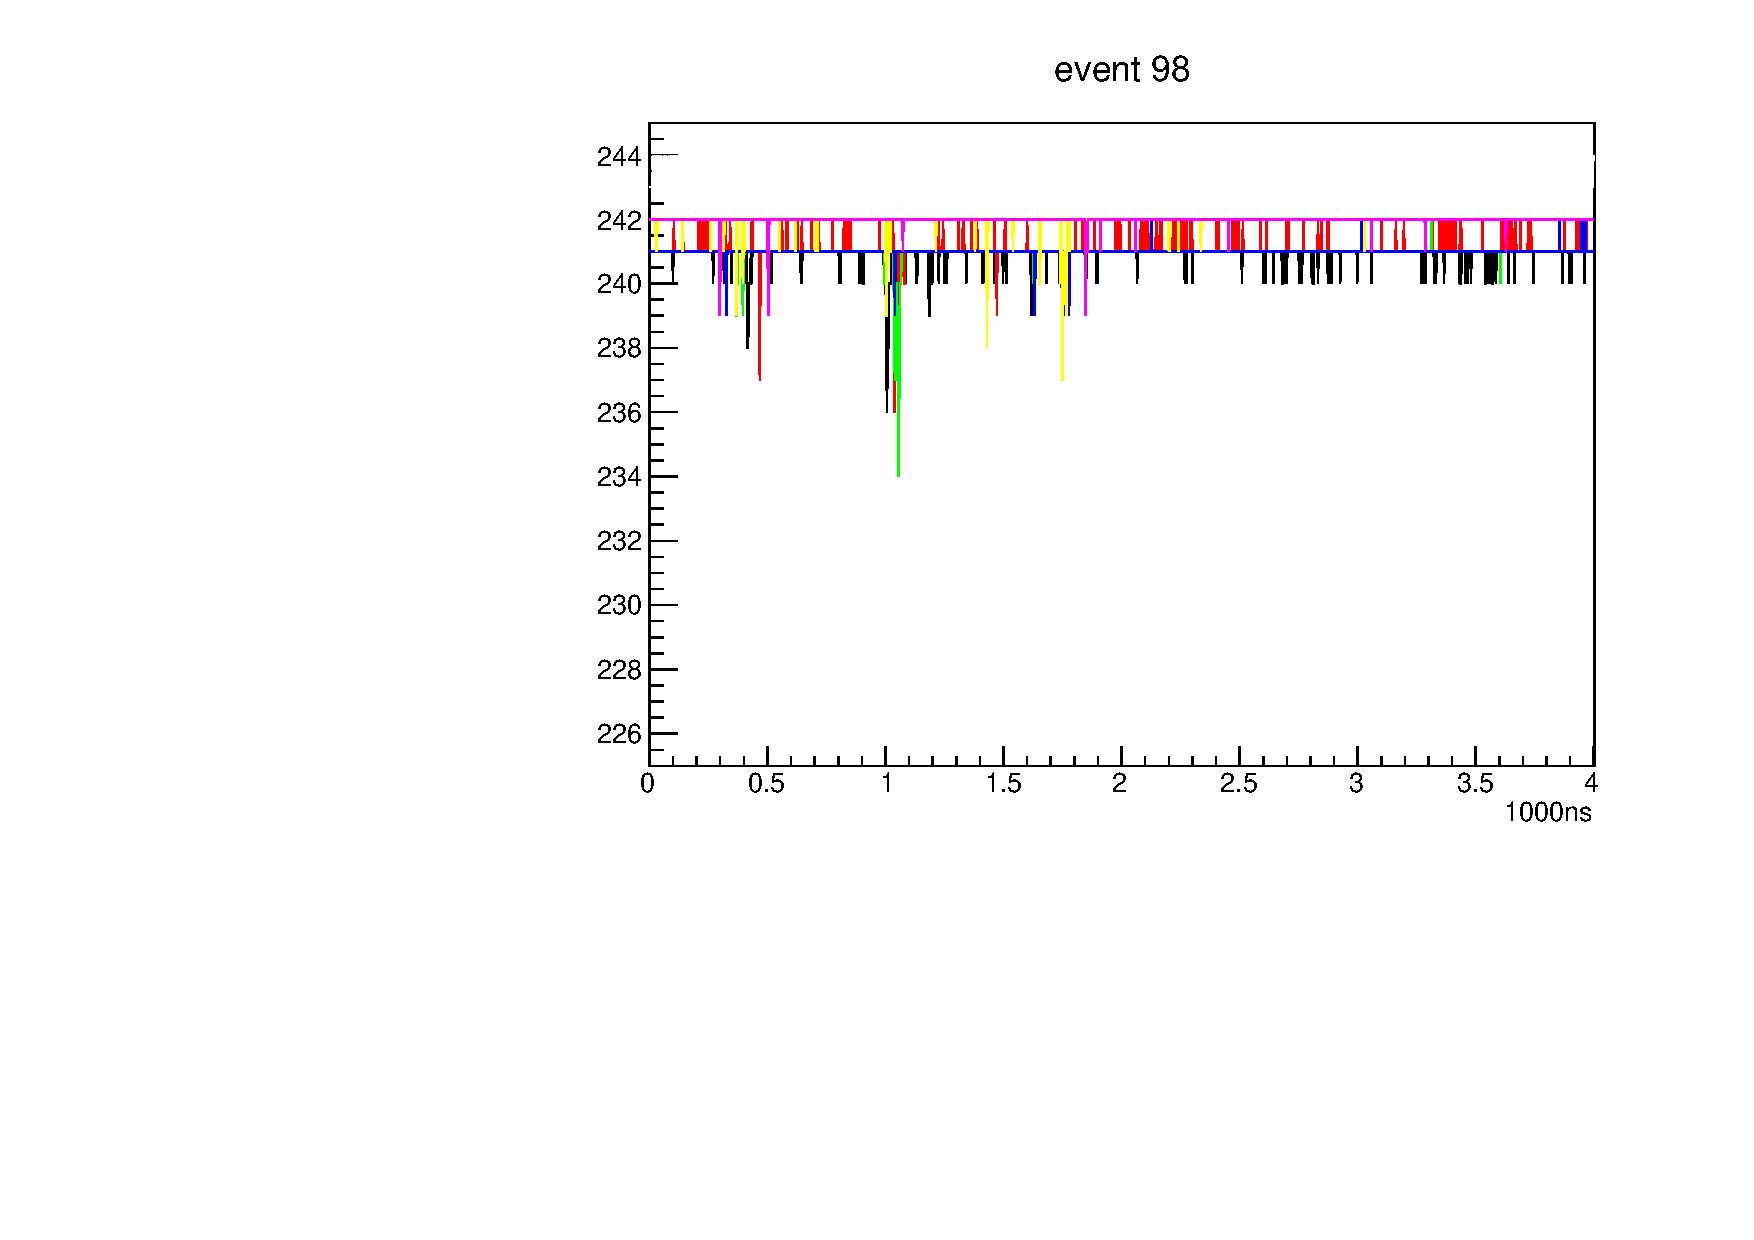
\includegraphics[width=0.8\textwidth,angle=-90]{figure/hayakawa/ps_plot.pdf}
\caption{PS 用のWFD で記録した波形}
\end{minipage}
\begin{minipage}{0.4\hsize}
\centering
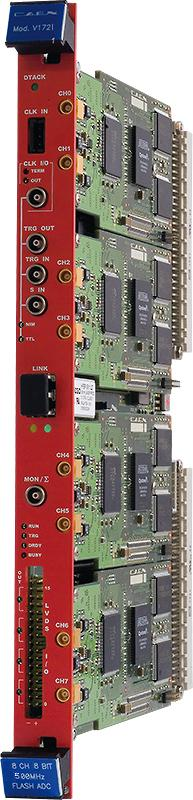
\includegraphics[width=0.2\textwidth]{figure/hayakawa/1095_L.jpg}
\end{minipage}
\end{tabular}
\end{figure}

\subsubsection{WFD (CAEN Waveform Digitizer DT5725)}
\begin{itemize}
\item 8~channel 14~bit 250~MS/s Digitizer
\item エネルギー分解能が良いので,主にエネルギー測定用のNaI 検出器の信号の記録に用いた
\item 9~本のNaI に対して8~チャンネルとチャンネル数が不足していたので,アナログ信号を合成して入力した
\end{itemize}
\begin{figure}[H]
\begin{tabular}{cc}
\begin{minipage}{0.5\hsize}
\centering
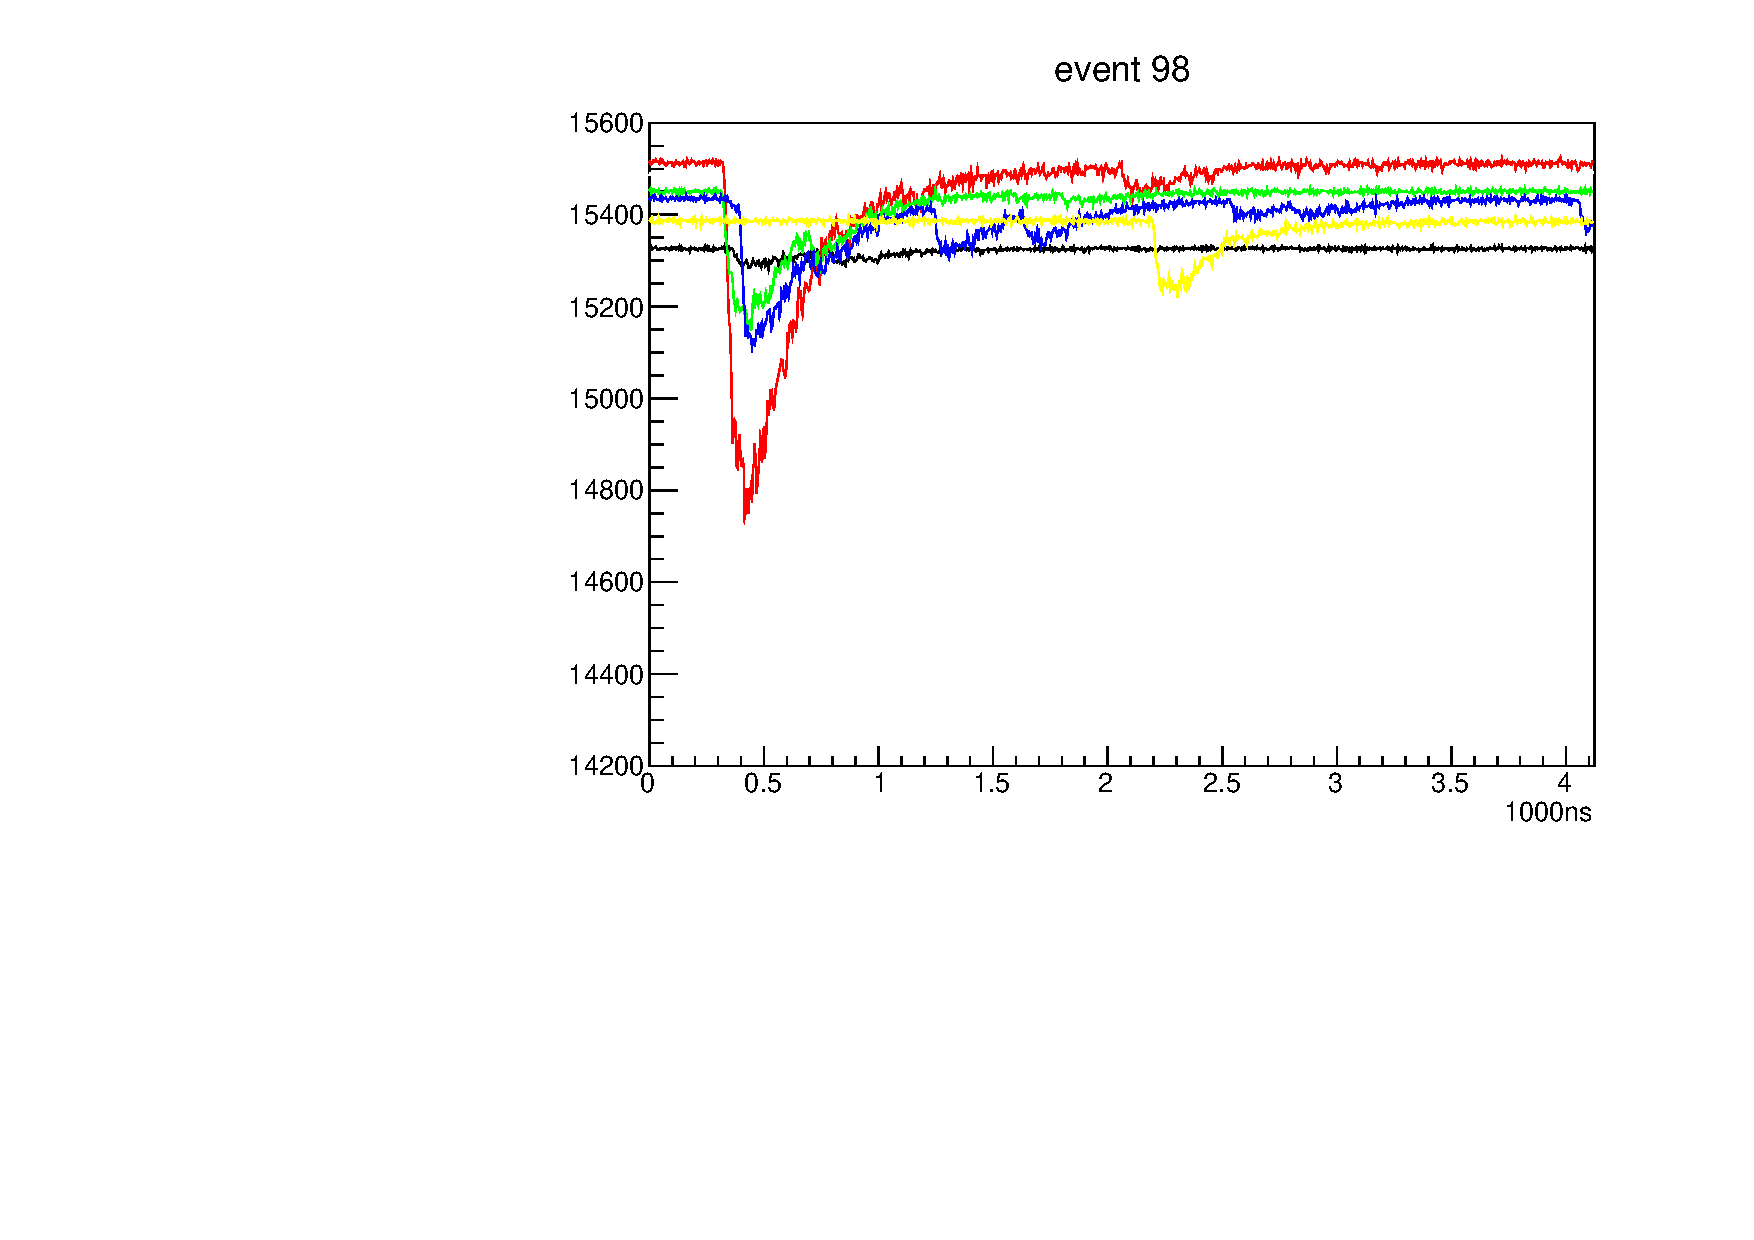
\includegraphics[width=0.8\textwidth,angle=-90]{figure/hayakawa/NaI_plot.pdf}
\caption{NaI 用のWFD で記録した波形}
\end{minipage}
\begin{minipage}{0.4\hsize}
\centering
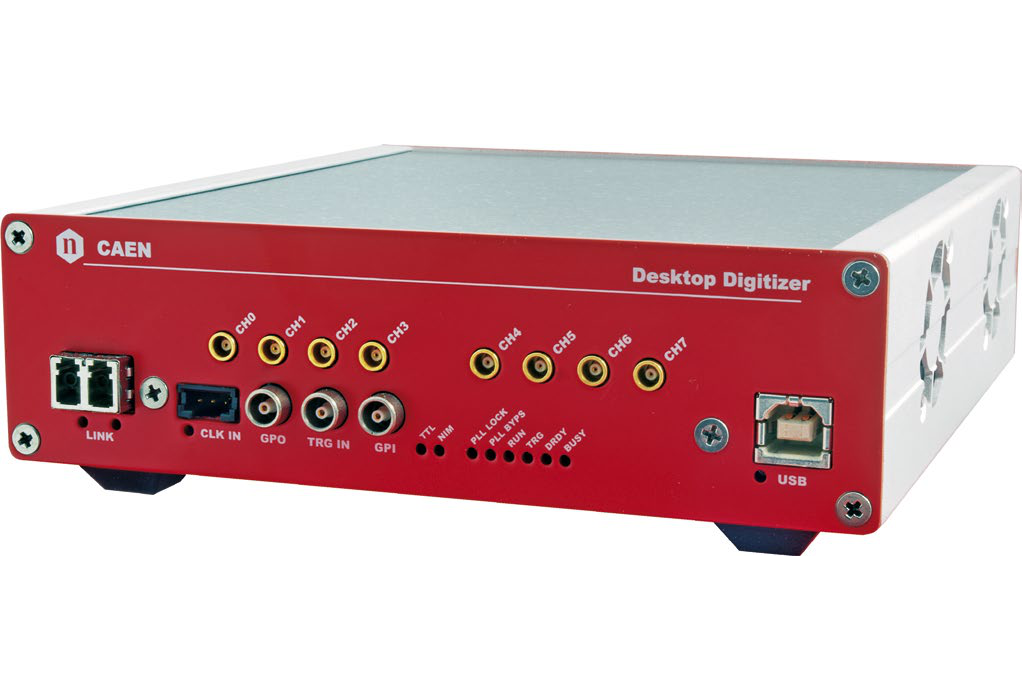
\includegraphics[width=0.6\textwidth]{figure/hayakawa/DT5725_L.png}
\end{minipage}
\end{tabular}
\end{figure}

%\end{document}

%\documentclass[uplatex,dvipdfmx]{jsarticle}

%\usepackage[dvipdfmx]{graphicx}
%\usepackage{graphicx}
%\usepackage{mathtools}
%\usepackage{cancel}
%\usepackage{amsmath,amssymb}
%\usepackage{cases}
%\usepackage{bm}

%\usepackage{here}
%\usepackage{colortbl}
%\usepackage{feynmf}

%\newcommand{\Slash}[1]{{\ooalign{\hfil/\hfil\crcr\(#1\)}}}

%\begin{document}

%\newpage
%\section{実験}
% -------キリトリ線(上)--------
\subsection{寿命測定のための銅板標的}
寿命測定に用いた銅板標的を図\ref{tar_cu}に示す.
これは厚さ$0.6\mathrm{mm}\times$横$280\mathrm{mm}\times$縦$120\mathrm{mm}$の銅板を木枠に固定したものである.
銅板の縦横の大きさはビームプロファイルからビームの広がりの約$3\sigma$になるように決めた.
厚さは$4[\mathrm{MeV}]$ミューオンが銅板の中心付近で止まるようなものを選んだ.
\subsection{$g$因子測定のための磁場装置}
$g$因子測定に用いた磁場印加標的を図\ref{tar_mag}に記す.
厚さ$0.6\mathrm{mm}\times$横$80\mathrm{mm}\times$縦$60\mathrm{mm}$の銅板を,呼び経$200\mathrm{mm}$の塩化ビニルパイプの中心にくるように紐で吊るした.
銅板の縦横の大きさはミューオンビームの広がりに対して約$1\sigma$の大きさになるように決めた.
磁石にはセラミック磁石(Y25)を用いており,磁石一束あたりの大きさは厚さ$9\mathrm{mm}\times$横$10\mathrm{mm}\times$縦$60\mathrm{mm}$である.
磁石はパイプの内側に接着剤で貼り付けたうえで,テープで補強した.

\begin{figure}[H]
  \begin{minipage}{0.45\hsize}
    \begin{center}
      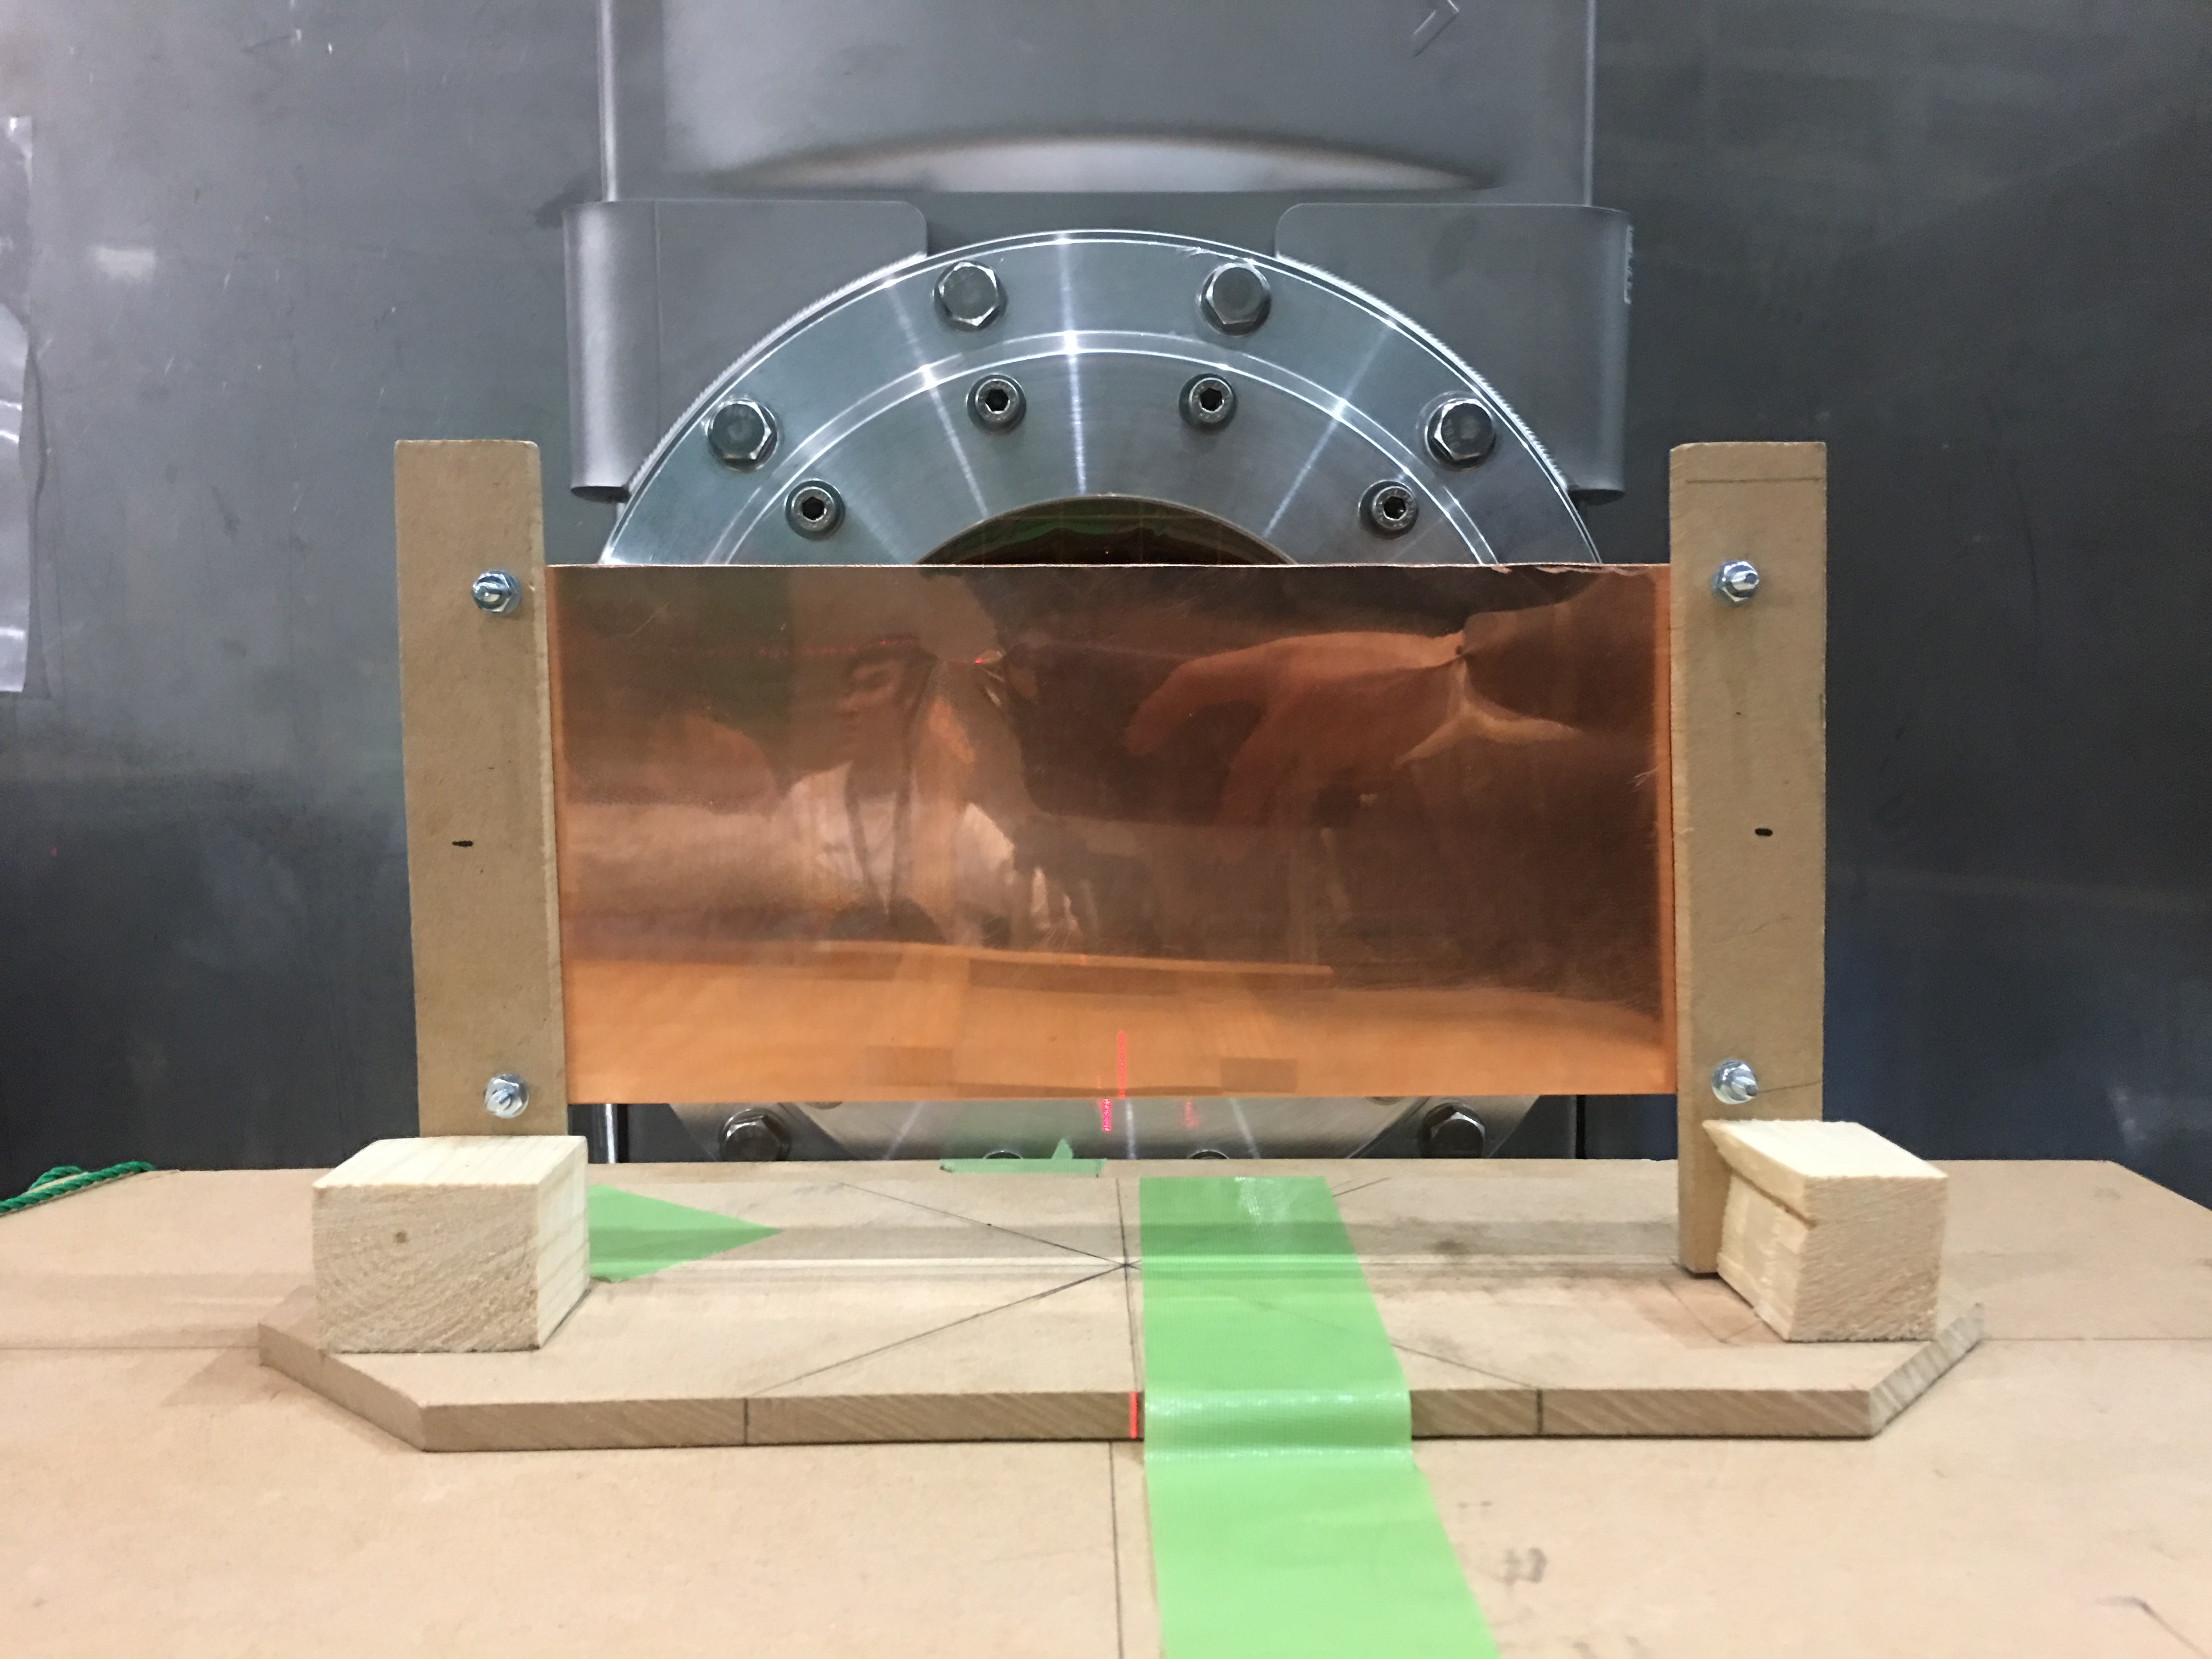
\includegraphics[width=1\textwidth]{figure/tajima/cu_target.jpg}
      \caption{銅板標的}
      \label{tar_cu}
    \end{center}
  \end{minipage}
  \hfill
  \begin{minipage}{0.45\hsize}
    \begin{center}
      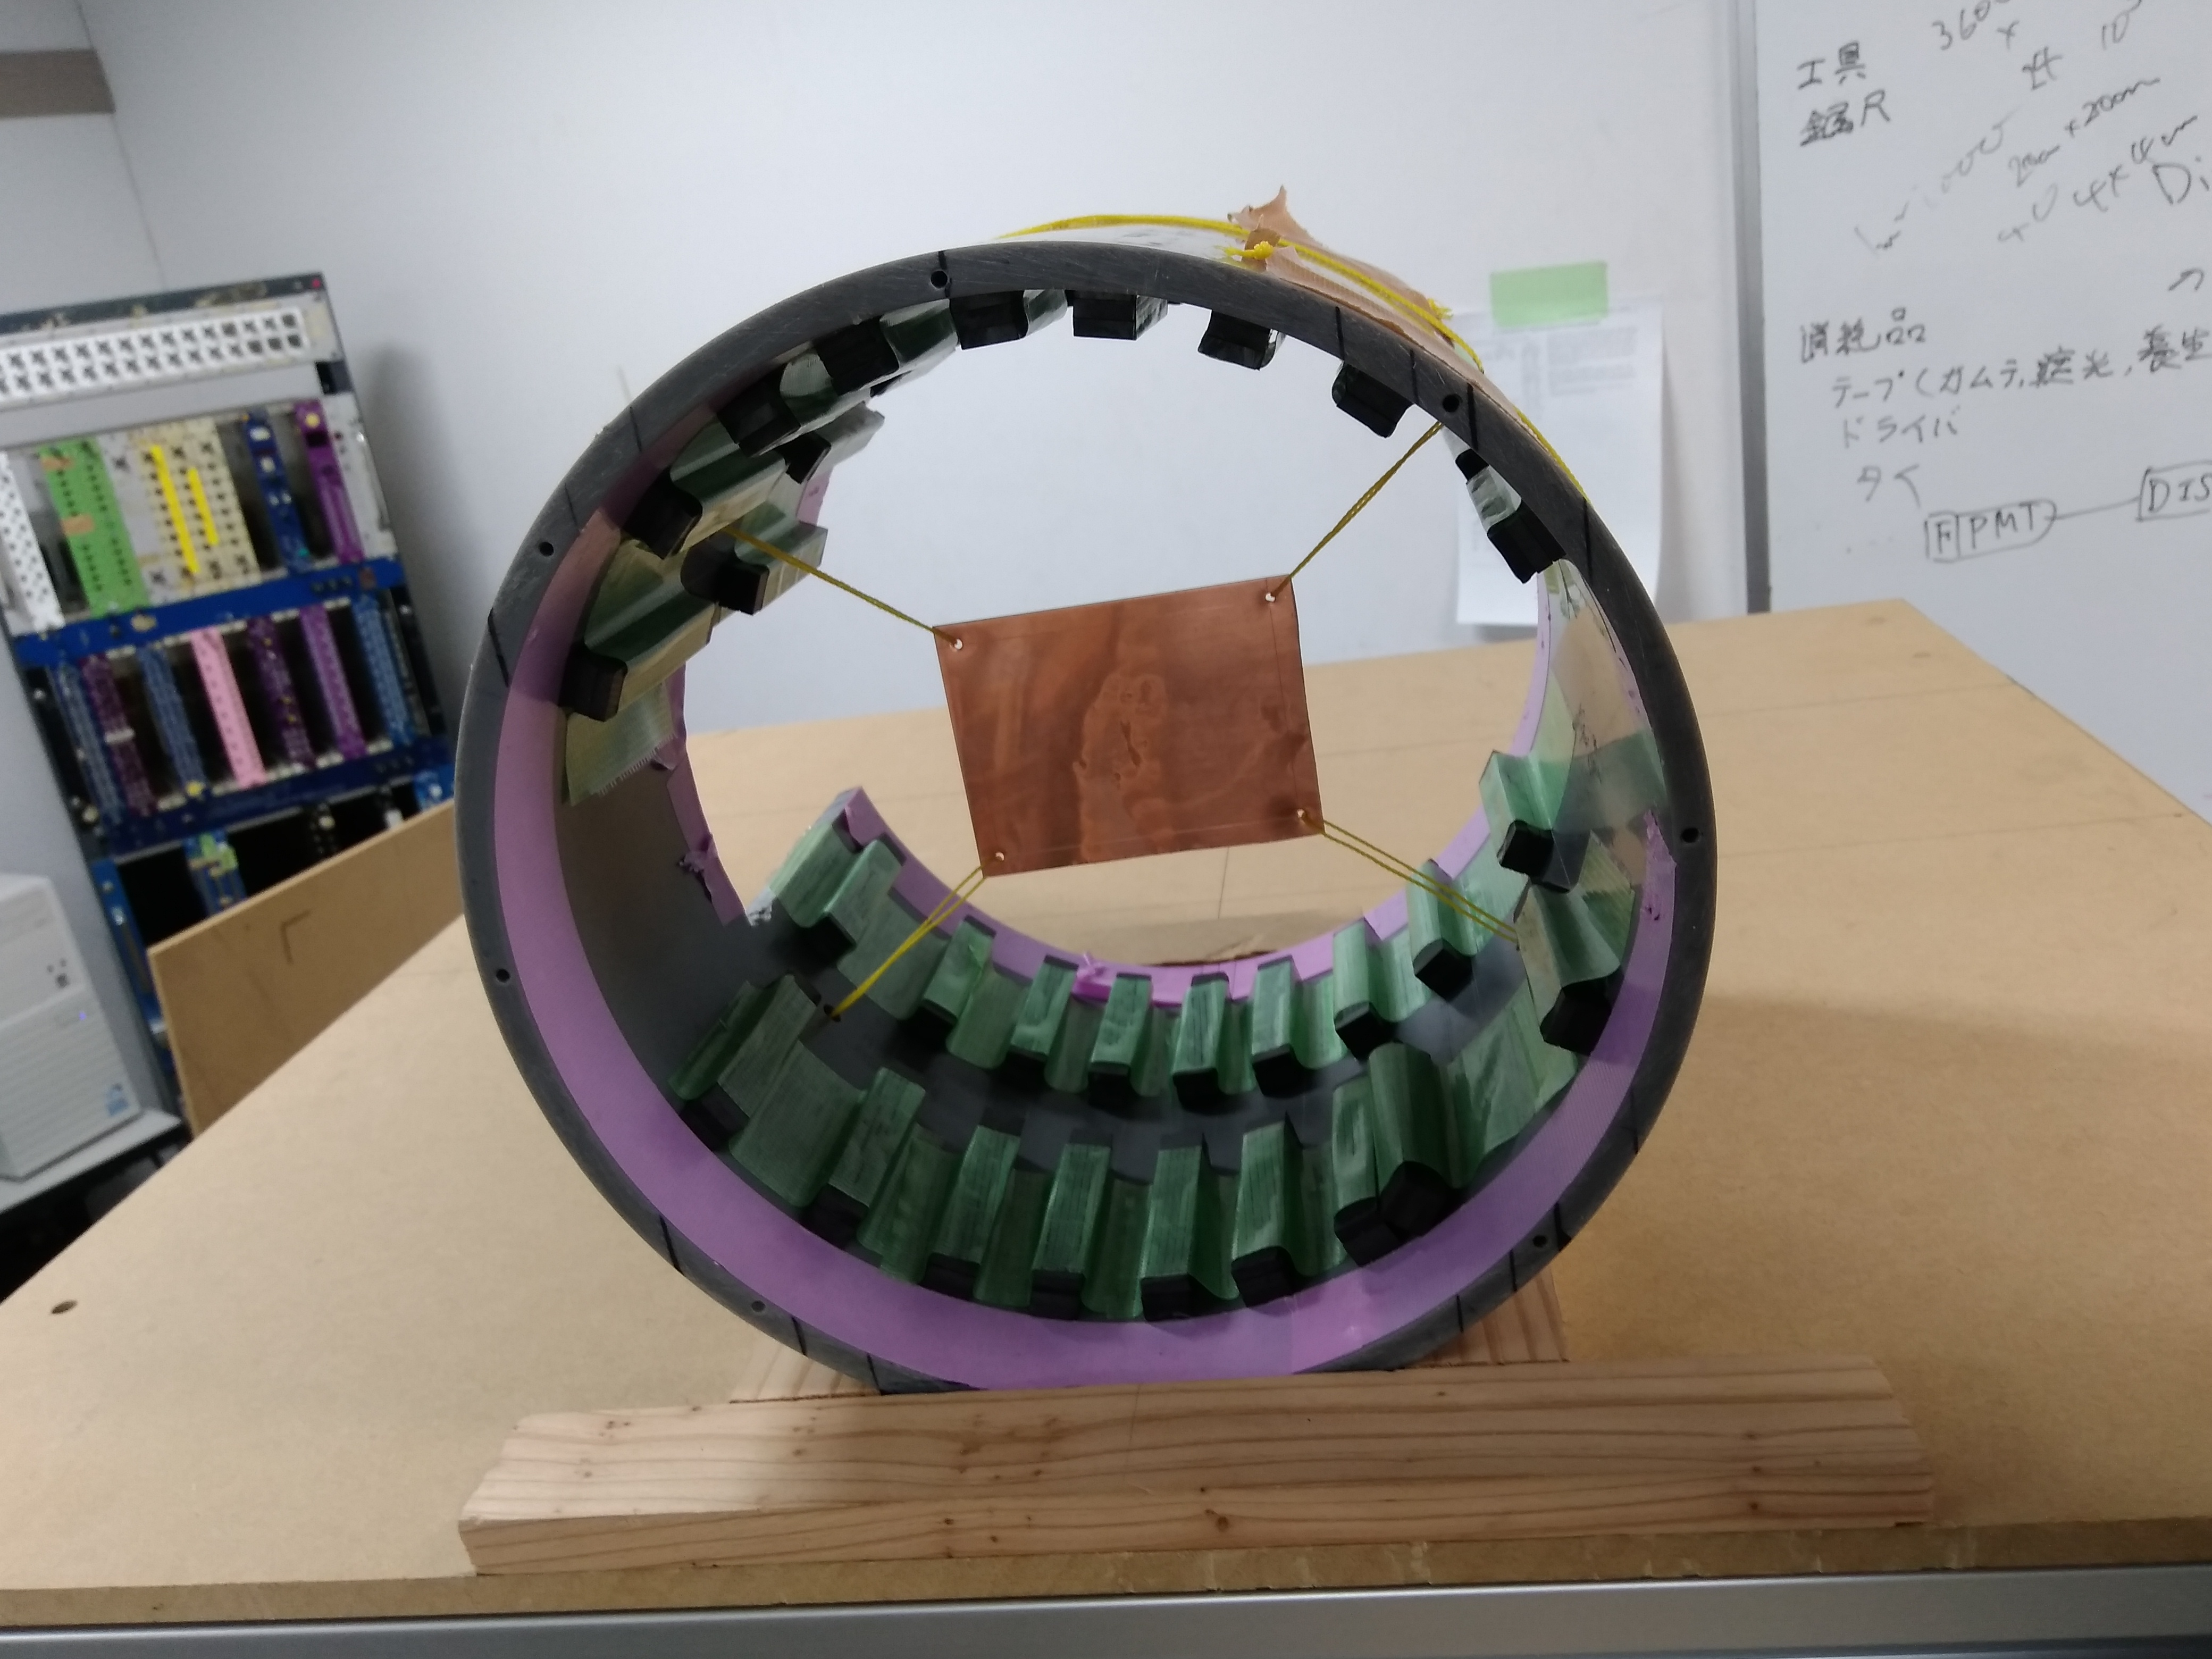
\includegraphics[width=1\textwidth]{figure/tajima/mag.jpg}
      \caption{磁場発生装置と標的 \protect\footnotemark}
      \label{tar_mag}
    \end{center}
  \end{minipage}
\end{figure}
\footnotetext{写真では下方の磁石が外れているが,これは後に修復した.}

\subsubsection{磁石の発生原理について: $\cos \theta$配置}
磁場装置は$\cos n\theta$巻き($n=1$)の電磁石を参考に作成した.
$\cos n \theta$巻きの電磁石の考え方は以下のものである.
下図\ref{cos2},\ref{cos4}のように,十分長い円環上を電流が$z$軸方向に流れているとする.
そして電流密度が$\cos n\theta$(ここで$\theta$は円柱座標($r,\theta,z$)における$\theta$で,$n$は整数)に比例したとする.
すると原点付近の領域に, $2n$極磁場が形成されるというものである.
導出の概略は,円環各点が形成する磁場をその点の周りでテーラー展開し,これを$\theta$について角度積分することで$2n$極磁場を形成する項のみが残るというものである.

\begin{figure}[H]
  \begin{minipage}{0.45\hsize}
    \begin{center}
      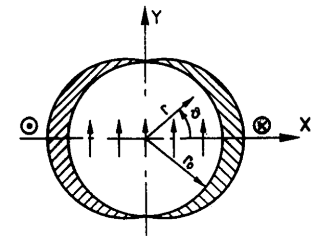
\includegraphics[width=0.8\textwidth]{figure/tajima/cos.png}
    \end{center}
    \caption{$\cos\theta$ : 2極磁石}
    \label{cos2}
  \end{minipage}
  \hfill
  \begin{minipage}{0.45\hsize}
    \begin{center}
      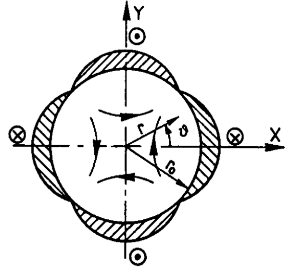
\includegraphics[width=0.7\textwidth]{figure/tajima/cos2.png}
    \end{center}
    \caption{$\cos2\theta$ : 4極磁石}
    \label{cos4}
  \end{minipage}
\end{figure}
%\renewcommand{\thefootnote}{\fnsymbol{footnote}}
\footnotetext{上図はKEKホームページ「加速器用超電導磁石(OHO11ogitsu20110906.pdf)」より引用}

作成の手軽さから,磁場発生源には電磁石ではなく永久磁石(セラミック磁石)を用いた.
電磁石における電流密度を,永久磁石の分布密度で置き換え,
磁石の分布密度が$|\sin\theta|$に比例するようにした.
$\sin\theta$としたのは磁石の向きをすべて動径方向に向けると,電磁石に比べ磁場の方向が$\pi/2$だけずれるためである.
また磁石の磁場方向は$0<\theta<\pi$と$\pi<\theta<2\pi$で動径方向に対して正と負になるようにした.
作成に入る前に考えた配置をFEMM\footnote{FEMM (Finite Element Method Magnetics)とは有限要素法を用いて2次元軸対称な電磁場や熱,電流などのシミュレーションを行うことができるソフトである.}を用いてシミュレートし,磁場の一様性を確認した.


実際に有限の長さの磁石で磁場装置を作成するにあたって,図\ref{tar_mag}のように磁石を長手方向に間隔を開けて二巻き配置した.
(一巻あたり磁石の数は18個である.)
長手方向の間隔は$30\mathrm{mm}$で,間隔を開けることにより長手方向に隙間を空けずに磁石を詰めたときに比べて,
磁力線が緩和され長手方向に磁場の一様性が増すと考えたためである.

\newpage
\subsection{予備実験}
%\subsubsection{プラスチックシンチレータの宇宙線較正}

\subsubsection{NaIのゲイン測定}
本実験で用いるNaIのセットアップの信号の数は,NaI 9本とフィンガーカウンターの計10個である.
一方でNaIの信号の処理に用いるFADCのチャンネル数は8つである.
このため,NaI+PMTからの信号をアナログで足し合わせてチャンネル数を絞る必要があった.
そこで8本のNaIについて2本1組のペアをつくり和をとることにし,
残りの1本に関しては和をとらずに真ん中に配置することにした.
そのためにはあらかじめ,足し合わせるペアの選定とGainの調整を行っておく必要があった.

まずNaI+PMTのゲイン測定するために,
HV値を変えながら線源$^{137}\mathrm{Cs}$の光電ピークを計11本のNaI+PMTで測定を行った.
これをそれぞれガウシアンでFittingし,得られた平均値をゲインとした.
さらにゲインについて以下の式が成り立つとし,両対数でFittingを行った.
\begin{equation}
\mathrm{Gain}[\mathrm{pC}]=a*\mathrm{HV}[\mathrm{kV}]^b  
\end{equation}
ただし$a, b$はFitting パラメータである.
その結果を図にしたものが図\ref{GainHV}で,
縦軸をゲインにあたる電荷$[\mathrm{pC}]$,横軸をHV値$[\mathrm{kV}]$とした.
また各HVでのエネルギー分解能とHVの関係をあらわした図が図\ref{HVreso}で,
縦軸を分解能,横軸をゲイン$[\mathrm{pC}]$とした.
ただし分解能はガウシアンの$\sigma$をチャージで割ったものある.
\begin{figure}[H]
  \begin{minipage}{0.45\hsize}
    \begin{center}\hspace*{-1em}
      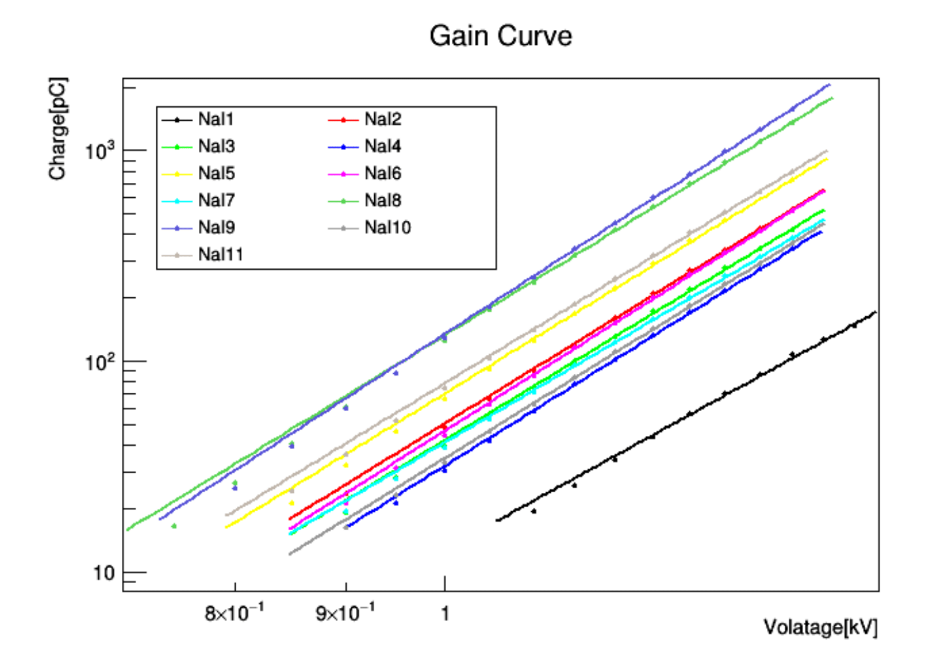
\includegraphics[width=1.1\textwidth]{figure/tajima/gain_curve.png}
    \end{center}
    \caption{GainとHVの対応}
    \label{GainHV}
  \end{minipage}
  \hfill
  \begin{minipage}{0.45\hsize}
    \begin{center}
      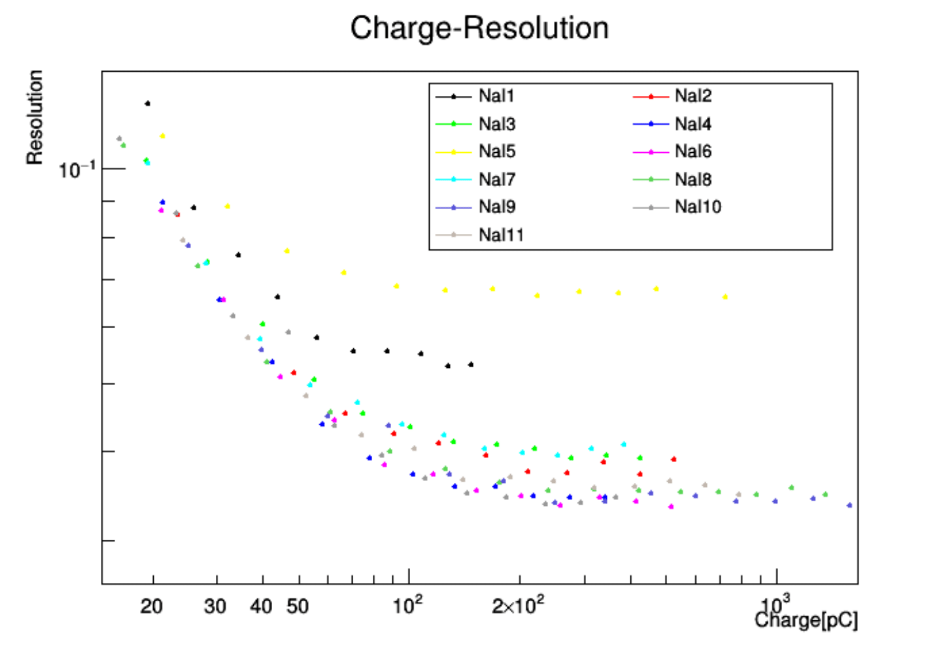
\includegraphics[width=1.1\textwidth]{figure/tajima/charge_resolution.png}
    \end{center}
    \caption{GainとResolutionの対応}
    \label{resoHV}
  \end{minipage}
\end{figure}
この結果, NaI1はゲインが低く,NaI5に関しては分解能が低かったため,本実験では用いないことにした.
(以降,NaI1,5で測定を行わないことにした.)
またNaI10は分解能が低かったため,足し合わせず真ん中に配置するNaIとした.

次に高いエネルギー領域においても,上のゲイン曲線が成り立っていることを確認するために,
ゲインが揃うようにHVを設定したうえで, 宇宙線を測定した.
そして,得られたチャージ分布をLandau関数をガウシアンで畳み込み積分した関数(以下,Langau関数とする.)で
Fittingをした.
この最頻値をゲインとすると,表\ref{nai_gain}のようになった.
このゲインの値が近く,またエネルギー分解能を近いものを足し合わせるペアとし,
これを(2,7),(3,9),(4,6),(8,11)の4組に決めた.
これらのペアのずれはいずれも$10\%$未満となった.

前に求めたゲイン曲線から本実験におけるHV値を表\ref{HV}となるように決めた.
崩壊電子の最大エネルギーである$\sim 50[\mathrm{MeV}]$が, FADCの上限の半分$1[\mathrm{V}]$($500[\mathrm{pC}$])になるように設定した.
\begin{table}[H]
  \begin{minipage}[t]{0.45\textwidth}
    \begin{center}
    \caption{宇宙線の測定結果}\label{nai_gain}
      \begin{tabular}{|c|c|}\hline
        NaI No. & Gain[pC]\\ \hline \hline
        2 & 2530 \\ \hline
        3 &2387 \\ \hline
        4 &2352 \\ \hline
        6 &2397 \\ \hline
        7  &2579 \\ \hline
        8  &2423 \\ \hline
        9  &2164 \\ \hline
        11  &2393 \\ \hline
      \end{tabular}
    \end{center}
  \end{minipage}
  \hfill
  \begin{minipage}[t]{0.45\textwidth}
    \begin{center}
    \caption{NaIのHV設定}\label{HV}
      \begin{tabular}{|c|c|}\hline
      NaI No.&HV[V]\\ \hline \hline
      % 1 & 1342 \\ \hline
      2 & 1050 \\ \hline
      3 & 1082 \\ \hline
      4 & 1125 \\ \hline
      % 5 & 1002 \\ \hline
      6 & 1062 \\ \hline
      7 & 1089 \\ \hline
      8 & 913 \\ \hline
      9 & 913 \\ \hline
      10 & 1112 \\ \hline
      11 & 984 \\ \hline
      \end{tabular}
    \end{center}
  \end{minipage}
\end{table}

さらに本実験におけるNaI+PMTの配置を表\ref{haichi}になるように決めた.
配置を決めるにあたって,以下の事柄を考慮した.
\begin{itemize}
\item エネルギー重心を求める観点からペアを中心から等距離になるように配置
\item 角でのGainが不足しないように, Gainの高いペアを角に配置
\item 本番セットアップでの宇宙線較正を想定して,上下にペアがこないように配置
\end{itemize}
\begin{table}[H]
  \begin{center}
    \caption{ビーム正面からみたNaIの配置図}\label{haichi}
    \begin{tabular}{|c|c|c|}\hline 
      \cellcolor{yellow}3&\cellcolor{red}2&\cellcolor{yellow}9\\ \hline
      \cellcolor{cyan}4&10&\cellcolor{red}7\\ \hline
      \cellcolor{green}8&\cellcolor{cyan}6&\cellcolor{green}11\\ \hline
    \end{tabular}
  \end{center}
\end{table}
\newpage
\subsubsection{NaIの宇宙線較正}
NaIでエネルギーを測定するために, 宇宙線較正を行った.
先にもとめたHV値のもとで,それぞれのNaIで宇宙線を測定した.
得られたチャージ分布を,Langau関数でFittingをした.(図\ref{langau})
そして得られた最頻値を宇宙線が落としたエネルギーとした.

次にGeant4を用いて,天頂角分布で宇宙線モンテカルロシミュレーションを行った.
図\ref{MC2}はシミュレーションによるエネルギー分布で,縦軸にカウント数,横軸にエネルギーを$24\mathrm{MeV}$で規格化したものをとった.
このエネルギー分布にLandau関数でFittingし,
得られた最頻値と測定によって得られた最頻値でエネルギー較正を行った.

\begin{figure}[H]
  \begin{minipage}{0.45\hsize}
    \begin{center}\hspace*{-1em}
  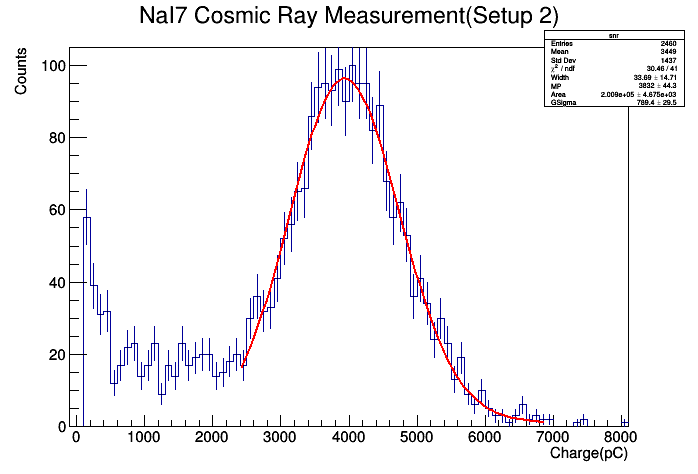
\includegraphics[width=1\textwidth]{figure/tajima/NaI7_Setup2.png}
      \caption{Langau Fitting}\label{langau}
    \end{center}
  \end{minipage}\hfill
  \begin{minipage}{0.45\hsize}
    \begin{center}
      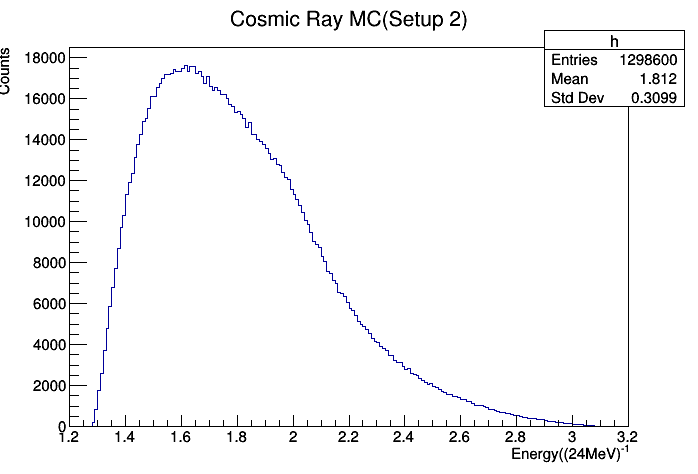
\includegraphics[width=1\textwidth]{figure/tajima/MC2.png}
      \caption{c}\label{MC2}
    \end{center}
  \end{minipage}
\end{figure}

図\ref{cali}は宇宙線較正の結果を図にしたもので,
縦軸をFADCで測定された電荷量$[\mathrm{pC}]$,横軸をエネルギー$[\mathrm{MeV}]$としたものである.
\begin{figure}[H]
  \centering
      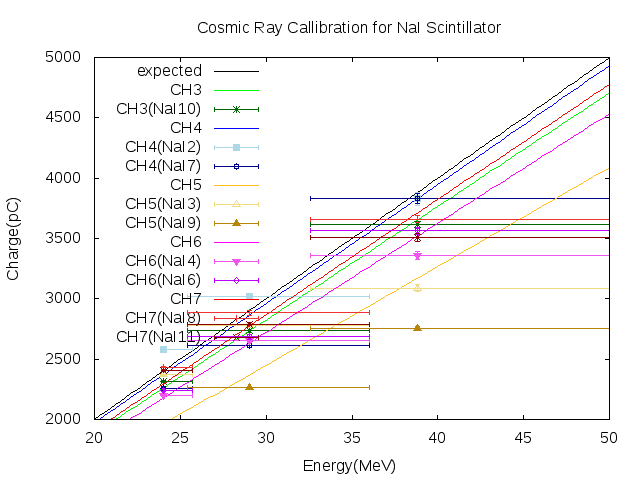
\includegraphics[width=0.7\textwidth]{figure/tajima/fit.png}
      \caption{宇宙線較正}\label{cali}
\end{figure}
\newpage
\subsubsection{磁場測定}
磁場装置の測定を行った.
3軸テスラメータで銅板を置く範囲を,$1\mathrm{cm}$間隔で計63点を測定した.
本実験の測定中に磁石が外れてしまったので,磁石が外れる前後で測定した. 

測定した結果を以下の表\ref{MF1},\ref{MF2}に記す.
$x,y$の単位は$[\mathrm{cm}]$で,磁場の単位は$[\mathrm{gauss}]$である.
原点を銅板の中心とし, $y,z$軸を鉛直方向上向きとビーム方向にとった.
\begin{table}[H]
  \begin{center}
    \caption{各点の磁場の強さ(磁石が外れる前)}\label{MF1}
    \begin{tabular}{|c||c|c|c|c|c|c|c|c|c|}\hline
       y\textbackslash x & -4 & -3 & -2 & -1 & 0 & 1 & 2 & 3 & 4 \\ \hline \hline
      3 & 51.48 & 54.98 & 55.33 & 55.55 & 55.42 & 54.77 & 54.44 & 53.27 & 51.75 \\ \hline
      2 & 56.25 & 56.78 & 56.87 & 56.84 & 56.41 & 56.16 & 55.93 & 55.71 & 55.35 \\ \hline
      1 & 57.15 & 57.50 & 57.39 & 57.11 & 56.72 & 56.53 & 56.48 & 56.50 & 56.44 \\ \hline
      0 & 57.60 & 57.49 & 57.19 & 56.72 & 56.54 & 56.48 & 56.53 & 56.58 & 55.98 \\ \hline
      -1 & 56.66 & 56.78 & 56.66 & 56.48 & 56.39 & 56.34 & 56.35 & 56.31 & 56.12 \\ \hline
      -2 & 53.45 & 54.74 & 55.29 & 55.54 & 55.60 & 55.60 & 55.53 & 55.14 & 54.3 \\ \hline
      -3 & 50.62 & 51.95 & 53.45 & 53.93 & 54.20 & 54.20 & 54.05 & 53.11 & 51.25 \\ \hline
    \end{tabular}
  \end{center}
\end{table}
\begin{table}[H]
  \begin{center}
    \caption{各点の磁場の強さ(磁石が外れた後)}\label{MF2}
    \begin{tabular}{|c||c|c|c|c|c|c|c|c|c|}\hline
       y\textbackslash x & -4 & -3 & -2 & -1 & 0 & 1 & 2 & 3 & 4 \\ \hline \hline
      3 & 55.41 & 55.93 & 55.79 & 54.78 & 53.30 & 50.73 & 46.89 & 46.34 & 41.95 \\ \hline
      2 & 57.25 & 57.06 & 56.28 & 54.92 & 53.77 & 52.01 & 49.83 & 48.45 & 48.44 \\ \hline
      1 & 57.72 & 57.30 & 56.52 & 55.61 & 54.34 & 52.97 & 51.84 & 51.08 & 50.49 \\ \hline
      0 & 57.55 & 56.94 & 56.30 & 55.54 & 54.61 & 53.67 & 52.98 & 52.40 & 52.34 \\ \hline
      -1 & 57.00 & 56.57 & 55.94 & 55.24 & 54.58 & 53.99 & 53.45 & 53.05 & 52.73 \\ \hline
      -2 & 55.48 & 55.37 & 55.04 & 54.64 & 54.30 & 53.83 & 53.39 & 52.53 & 51.81 \\ \hline
      -3 & 52.23 & 53.03 & 53.28 & 53.29 & 53.18 & 52.71 & 52.00 & 51.51 & 50.12 \\ \hline
 \end{tabular}
  \end{center}
\end{table}
有効な磁場を得るために,予め頂いたビームプロファイルのデータ($\sigma_x=33.3037[\mathrm{mm}],\ \sigma_y=19.6668[\mathrm{mm}]$)を用いて
加重平均をとった.
結果,磁石が外れる前後の磁場がそれぞれ$56.06\pm 1.20\  [\mathrm{gauss}]$ と$53.97\pm 2.36\  [\mathrm{gauss}]$ と求まった.
\newpage
\subsection{ビームを用いた本実験}
\subsubsection{タイムスケジュール}
本実験におけるタイムスケジュールは以下の通りである.
\begin{itemize}
\item 2/25 (Sun.)\\
  13:00   東海村到着,前日準備
\item 2/26 (Mon.) $\sim$ 2/27 (Tue.)\\
  9:00 $\sim$ロシアグループの傍らで寿命を測定, セットアップの確認
\item 2/28 (Wed.)\\
  12:30   ロシアグループの実験終了,\ P2ターゲットで実験開始\\
  12:30 - 21:30 セットアップの確認\\
  21:47 - 24:00 磁場ターゲットを置いて,\ $g$因子をNaIのみで測定\\
  24:20 - 29:50 磁場ターゲットを置いて,\ $g$因子をPSを加えて測定(測定の途中で磁石が外れる)
\item 3/1 (Thu.)\\
  7:20 - 8:10 銅板標的を置いて, エネルギーと寿命を測定\\
  8:30   ビームストップ\\
  8:30 - 14:30 放射線チェック, 片付け \\
  14:30 $\sim$ 帰宅
\end{itemize}
\subsubsection{セットアップ}
%本実験の寿命測定におけるセットアップを図\ref{set_lifetime}に記す.
%\begin{figure}[H]
%  \centering
%  \includegraphics[width=0.7\textwidth]{figure/tajima/lifetime.png}
%  \caption{寿命測定のセットアップ}
%  \label{set_lifetime}
%\end{figure}
この節では本実験のセットアップについて記す.\\
まず寿命測定のセットアップについて図\ref{set_life},\ref{set_life2}に記す.
図\ref{set_life}が上空からみたセットアップ図で,図\ref{set_life2}が実際のセットアップの写真である.
ここでFC, PSはフィンガーカウンターとプラスチックシンチレータの略で, Targetには先に述べた銅板標的を用いた.
ターゲットから測定器までの距離は,ビーム$1[\mathrm{pulse}]$あたりの陽電子のカウント数からきめた.
\begin{figure}[H]
  \begin{minipage}{0.45\hsize}
    \begin{center}
      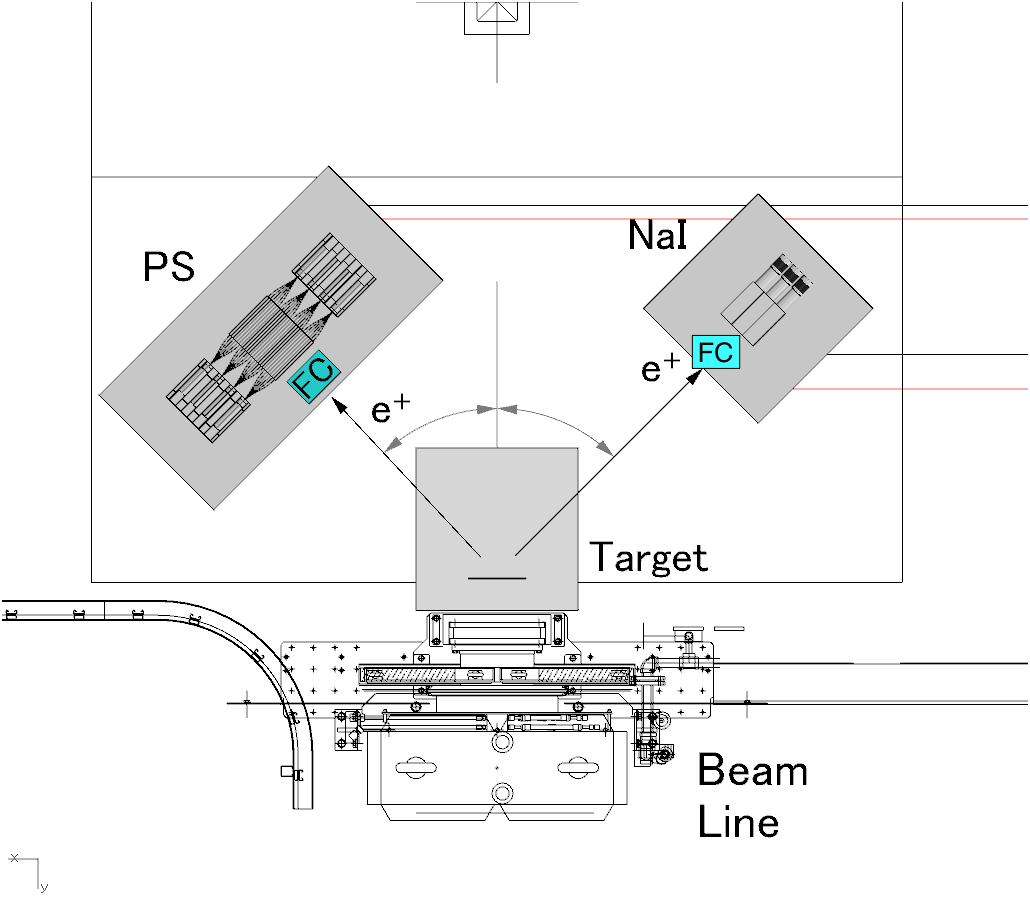
\includegraphics[width=1\textwidth]{figure/tajima/set_lifetime.png}
      \caption{寿命測定のセットアップ図}
      \label{set_life}
    \end{center}
  \end{minipage}
  \begin{minipage}{0.45\hsize}
    \begin{center}
      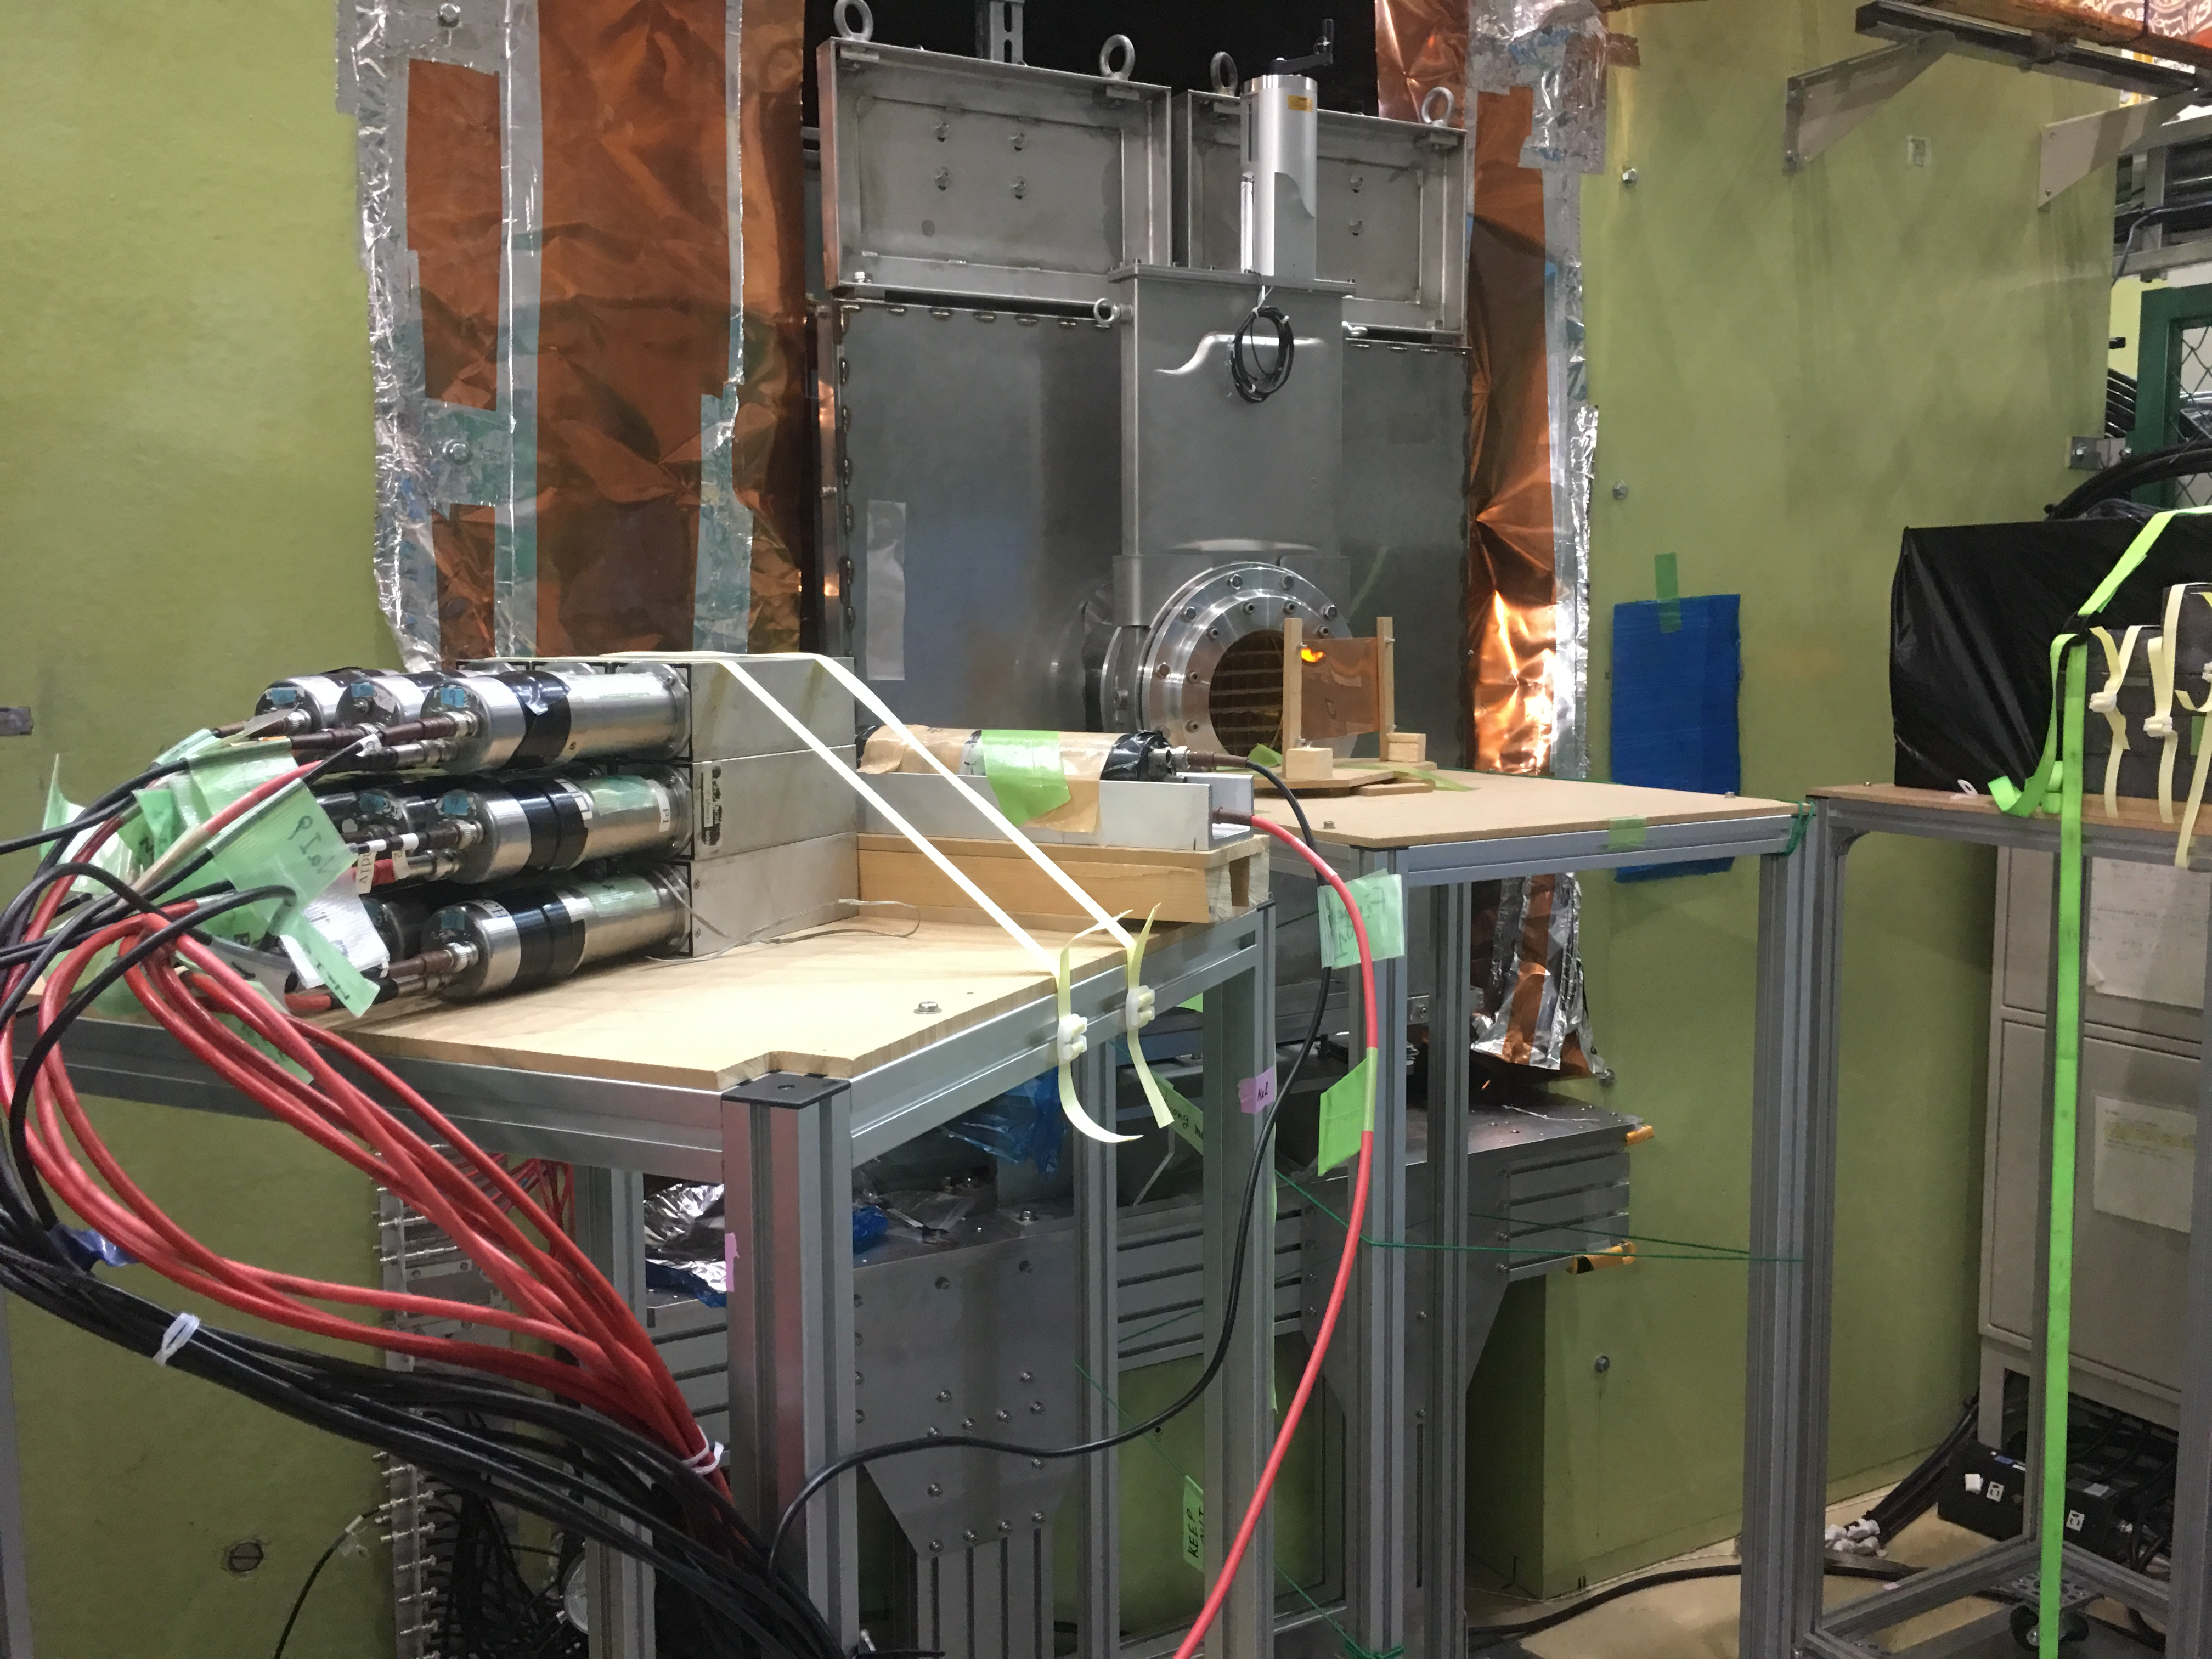
\includegraphics[width=1\textwidth]{figure/tajima/set_lifetime_1.png}
      \caption{寿命測定のセットアップ(写真)}
      \label{set_life2}
    \end{center}
  \end{minipage}
\end{figure}

次にエネルギー, $g$因子測定のセットアップについて図\ref{set_g_1}.\ref{set_g_2}に記す.
図\ref{set_life}が上空からみたセットアップ図で,図\ref{set_life2}が実際のセットアップの写真である.
ここでTargetには先に記した磁場印加標的を用いた.
寿命測定と同様に,ターゲットから測定器までの距離は,ビーム$1[\mathrm{pulse}]$あたりの陽電子のカウント数から決めた.
\begin{figure}[H]
  \begin{minipage}{0.45\hsize}
    \begin{center}
      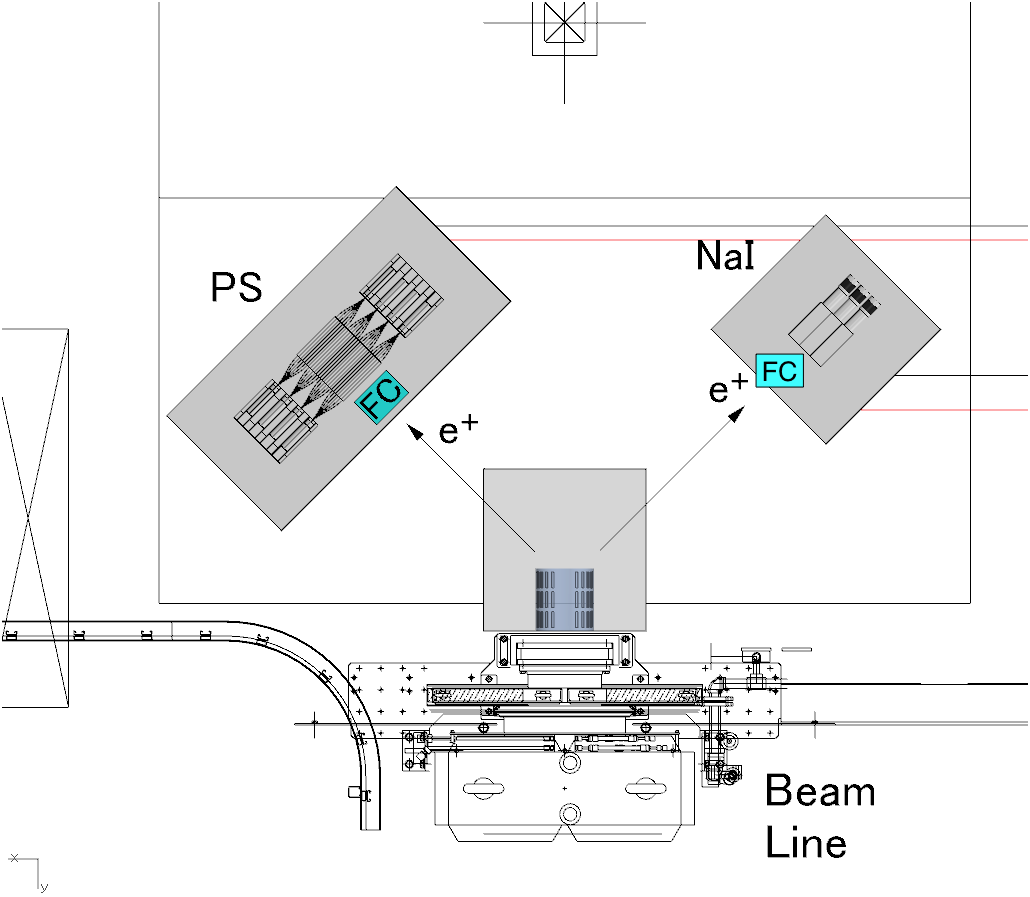
\includegraphics[width=1\textwidth]{figure/tajima/g-2_3.png}
      \caption{$g$因子測定のセットアップ}
      \label{set_g_1}
    \end{center}
  \end{minipage}
  \begin{minipage}{0.45\hsize}
    \begin{center}
      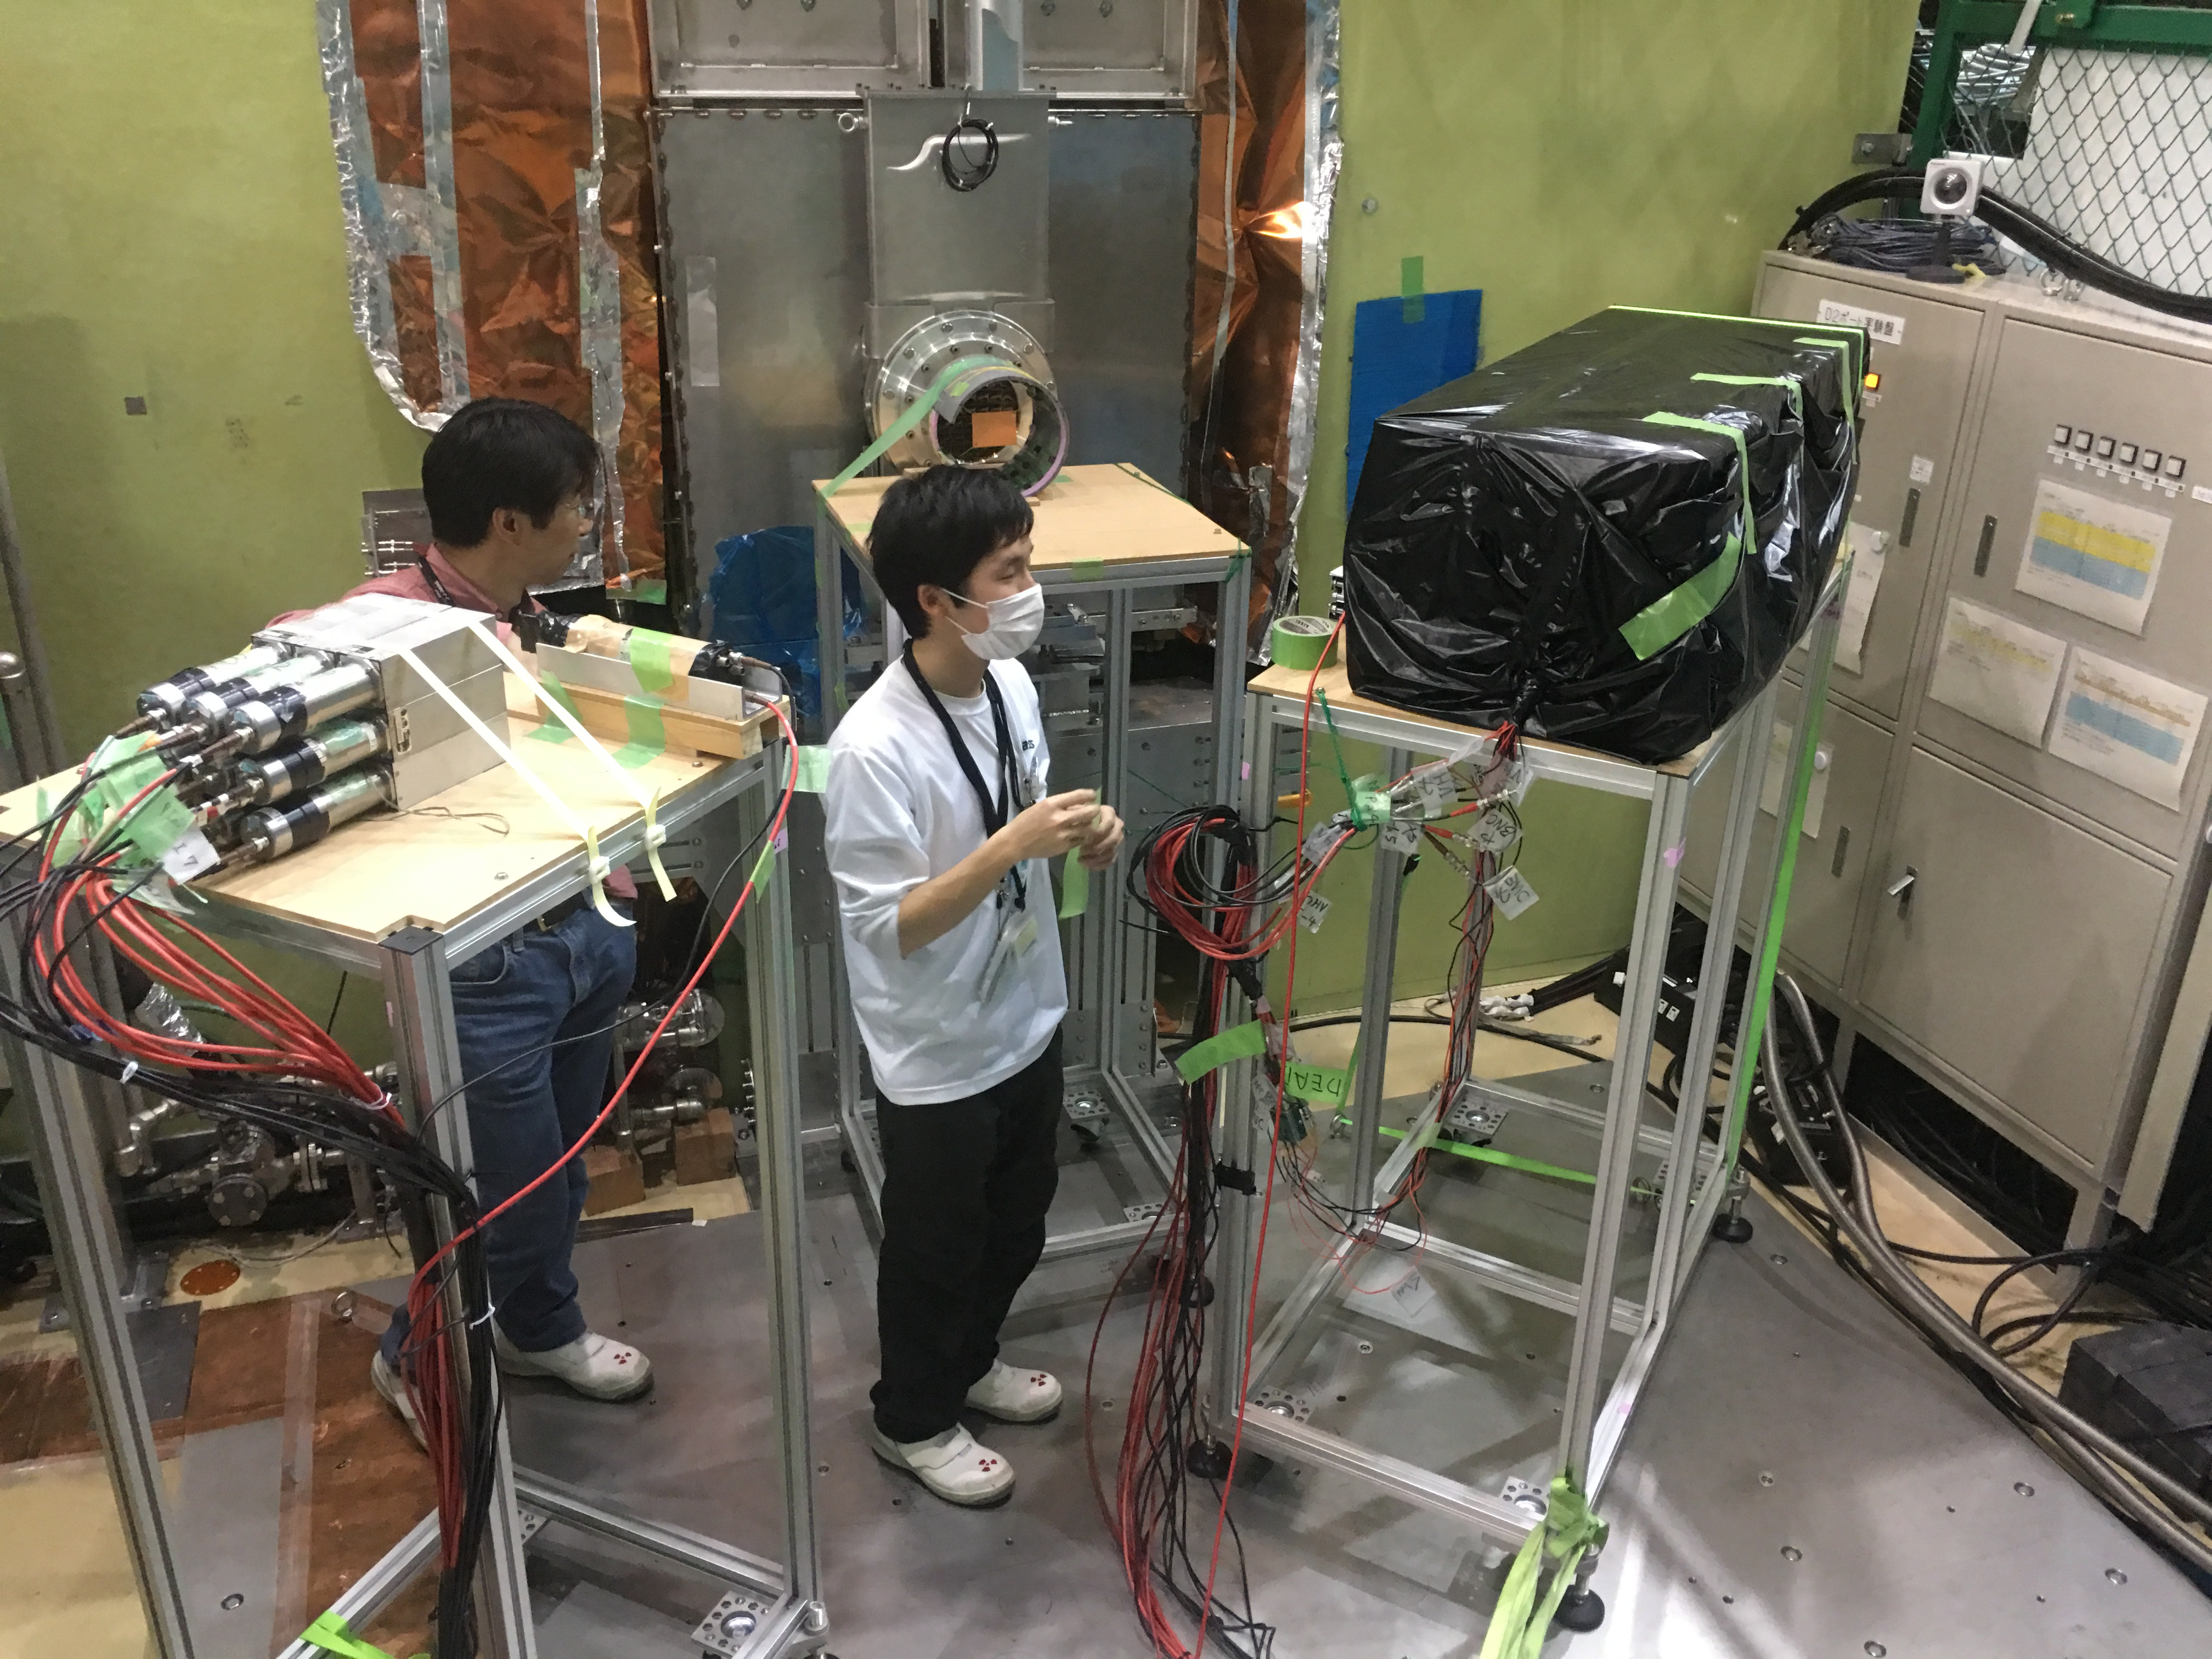
\includegraphics[width=1.1\textwidth]{figure/tajima/g.jpg}
      \caption{$g$因子測定のセットアップ(写真)}
      \label{set_g_2}
    \end{center}
  \end{minipage}
\end{figure}
\subsubsection{回路}
この節では本実験の回路について述べる.\\
図\ref{cir_PS},\ref{cir_nai}はNaI,プラスチックシンチレータの回路である.
ここでBeam TrigerはMLF施設からの信号で,FADCの外部Trigerとして接続した.
また図\ref{cir_PS}の$n-s$($n=1,2,3,4$, $s=a,b$)はプラスチックシンチレータの$n$層目のファイバーの片側から読み出される信号を意味する.
図中に記載している端子名(BNC, LEMO, MCX)は接続したケーブルの両端の端子名である。
\begin{figure}[H]
  \begin{minipage}{0.45\hsize}
    \begin{center}
      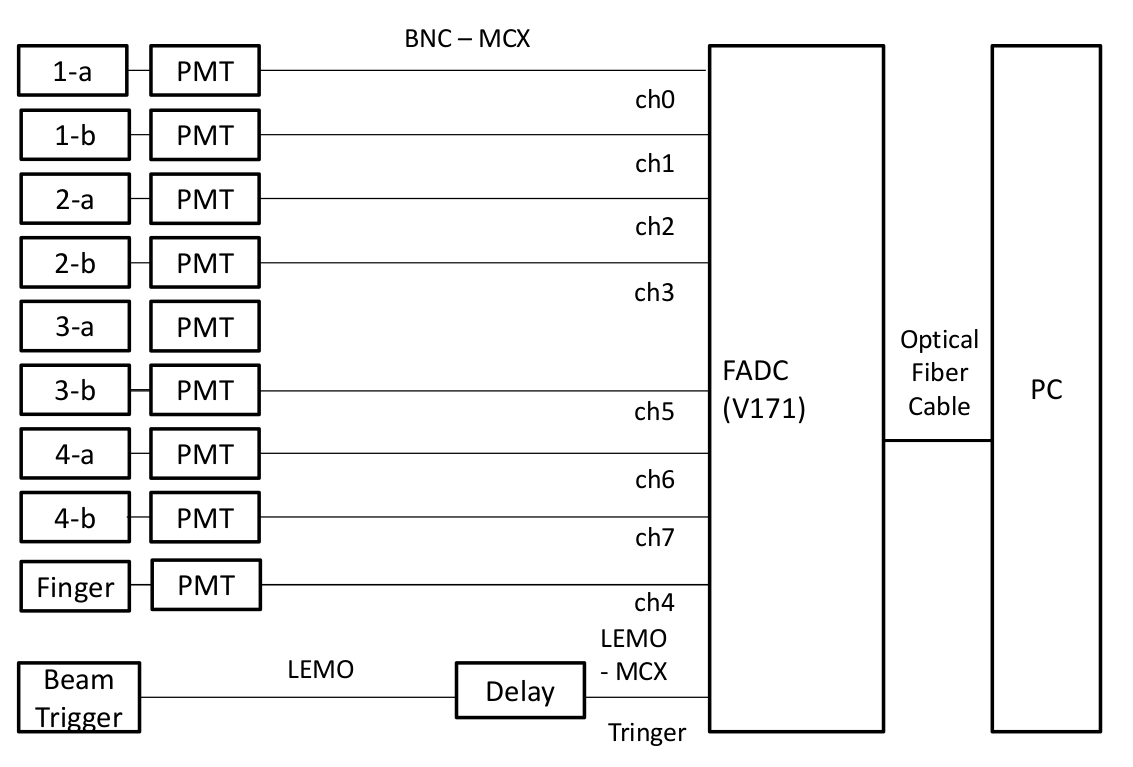
\includegraphics[width=1\textwidth]{figure/tajima/circuit_ps_2.png}
      \caption{プラスチックシンチレータの回路}
      \label{cir_PS}
    \end{center}
  \end{minipage}
  \hfill
  \begin{minipage}{0.45\hsize}
    \begin{center}
      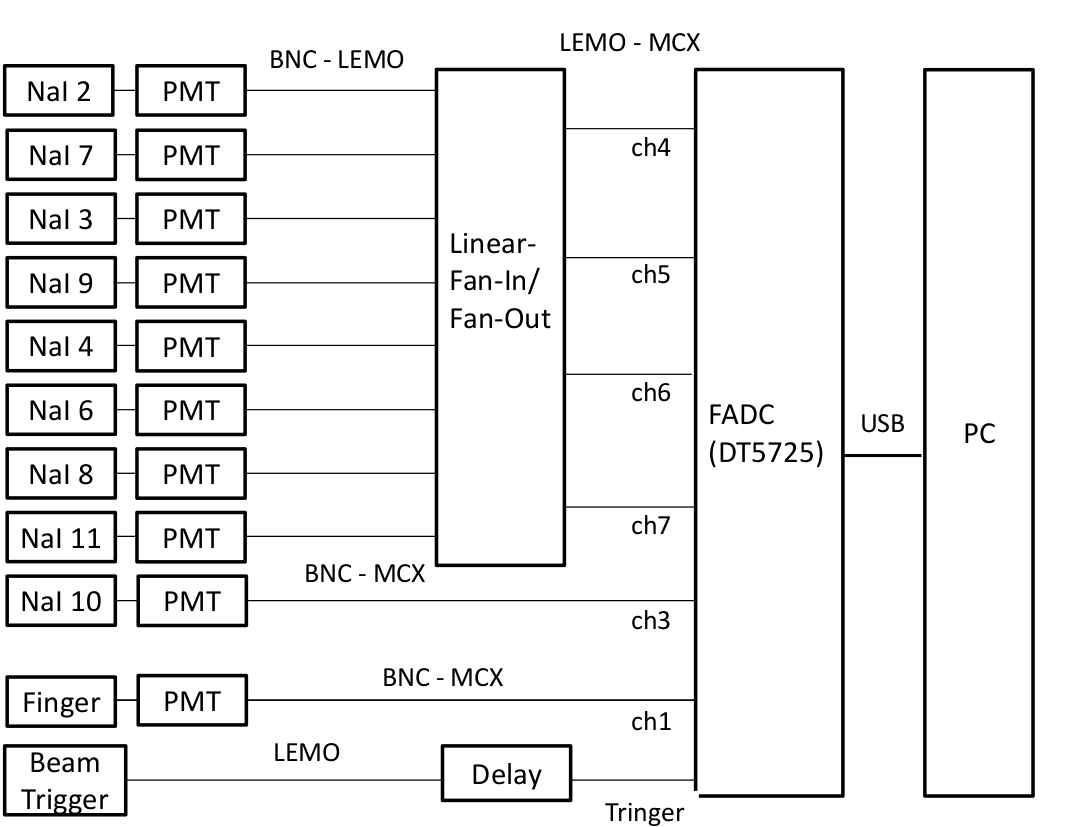
\includegraphics[width=1\textwidth]{figure/tajima/circuit_nai.png}
      \caption{NaIの回路}
      \label{cir_nai}
    \end{center}
  \end{minipage}
\end{figure}
本実験ではターゲットからの陽電子かを厳しく見積もるために,
プラスチックシンチレータにおいてもフィンガーカウンターを設置する必要性が浮上した.
そこでフィンガーカウンターを設置して,プラスチックシンチレータの3層目を片側読み出しにすることにした.

\subsubsection{実験手順}
本実験は以下の手順で行った.
\begin{enumerate}
  \item セットアップを調整
  \item ビームエリアの施錠を行い,ビームラインを開放
  \item ビームライン上のコリメーターを制御することで, \\ビーム1パルス当たりのレートを調整
    \\必要な場合はセットアップ調整からやり直した
  \item FADCでデータテイキング開始
\end{enumerate}
%--------キリトリ線(下)--------
%\end{document}

%\documentclass[titlepage]{jsarticle}

%\usepackage[dvipdfmx]{graphicx}

%数式用パッケージ
%\usepackage{amsmath, amssymb}
%\usepackage{mathtools}
%\usepackage{cancel}
%\usepackage{cases}
%\usepackage{bm}
%\usepackage{array,booktabs}
%\usepackage{float}

%\usepackage{subcaption}

%ファインマングラフ用パッケージ
%\usepackage{feynmf}



%\graphicspath{{./figure/}}

%\begin{document}

%%%%%%%%%%%%%%%%%%%池満パート開始%%%%%%%%%%%%%%%%%%%
\section{プラスチックシンチレータで取得したデータの解析と考察}
プラスチックシンチレータのデータの解析では波形解析やイベント選択の手法の異なる2つの解析手法を行った.それぞれで寿命と$g$因子の2つを求めた.
以下ではそれぞれに解析手法Aと解析手法Bと名付けた.また,最後に両方の結果をまとめた.

\subsubsection{解析手法A}
プラスチックシンチレータ(以下、PS)検出器を用いて取得したデータを以下の方法で解析し、寿命、$g$因子、エネルギー分布を求めた。
\begin{enumerate}
\item イベントディスプレイから、初めの100 (ns) (50 Sample)の間は信号が来ていないことを確認し、0〜100 (ns) のデータの平均値をとってそれをbaselineとした.
\item 信号のしきい値(threshold)の決定
\begin{itemize}
\item 宇宙線を用いた予備実験の結果から,12(MeV) のエネルギーに対応する信号のピーク値を求めた.%宇宙線を用いた予備実験の説明は?? 12MeVがMIPがPSの厚さを通った時に落とすエネルギーである説明.
\item そのピーク値から、各チャンネルごとのthresholdを以下の値に決めた.
\item 寿命測定と$g$因子測定用には、1層目:3 MeV相当、2層目以降:2 MeV相当とした.
\item エネルギー測定用には、1層目:4 MeV相当とし、2層目以降はthresholdを設けなかった.%なぜ?
\end{itemize}
\item 各チャンネルごとで,thresholdを越えた時間を信号の時間(peaktime)とした.
\item イベントディスプレイからおおよその信号の時間幅を決め、信号が検出されてから次の信号を検出するようになるまでのveto時間を40 ns にした.
\item peaktimeから40 ns の間のデータを足すことで信号のchargeを求めた.
\item 寿命と$g$因子について
\begin{itemize}
\item 各層の両側のチャンネルの信号のcoincidenceを取った.ただし、3層目は片側のみの信号である.
\item ここでcoincidenceの条件は,互いのpeaktimeが10 ns よりも近いものとした.
\item 寿命測定では,層ごとのcoincidenceのみをとった.
\item $g$因子測定では,立体角を制限するために、層ごとだけでなくフィンガーカウンターとのcoincidenceを要求した。
\end{itemize}
\item エネルギーについて
\begin{itemize}
\item 予備実験のデータから,各チャンネルごとにキャリブレーションをした.%上に同じ,実験説明が無い.
\item 各層のエネルギーとして,1,2,4層目では両側のチャンネルのエネルギーの平均を取り、3層目では片方のチャンネルのエネルギーを使用した.
\item fingerと1層目の両側のチャンネルの信号のcoincidenceをとり,そのときの全層のエネルギーの和を求めた.
2層目以降のチャンネルで信号がない場合,そのチャンネルのエネルギーは0とした.
\item fingerとのcoincidenceを取ったのは,検出器の中心に入ったe$^{+}$の信号のみを選択し,エネルギー漏れを減らすためである.%エネルギー漏れとは?
\end{itemize}
\end{enumerate}

\subsubsection{信号検出のthreshold値について}
この小節の後で解析の結果を述べるが,その前に信号検出時のthresholdの値の判断理由について触れておく.

まず,1層目の信号の中には,標的に当たらずにビーム出口から直接検出器に入るミューオンによる信号があると考えた.
1層目のthresholdを他層よりも高く設定しているのは,このようなバックグラウンドを除去するためである.%なぜ除去できる?

次に,thresholdの値を1MeV相当にして寿命を求めると,thresholdが高いときよりも長くなった.
よって,1MeV相当のthresholdでは低エネルギーのノイズを信号として処理していると考えた.
一方,寿命測定に関して,thresholdを上げてもfittingの結果は変わらず,統計誤差が大きくなるだけだった.%表現に違和感

以上のことを基にして,thresholdの値を判断した.

\subsubsection{得られた崩壊曲線とfittingの結果}
図\ref{lt_layercoin}は,磁場なし標的を用いたときのミューオンの崩壊曲線である.
それを次の$f_{\mathrm{life}}(t)$でfittingした結果が図\ref{lt_layercoin_fit}である.
\begin{equation*}
f_{\mathrm{life}}(t) = \exp[-(t+A)/\tau].
\end{equation*}
また,図\ref{g_layercoin}は磁場あり標的を用いたときのミューオンの崩壊曲線である.
それを次の$f_{g}(t)$でfittingした結果が図\ref{g_layercoin_fit}である.
\begin{equation*}
f_{g}(t) = \exp[-(t+A)/\tau](1+B\cos(\omega t + \delta)).
\end{equation*}

fittigの結果は表\ref{fit_lt},\ref{fit_g}のようになった.表中の誤差はfittingに由来する統計誤差である.

\begin{table}[H]
\caption{寿命$\tau$のfitting結果}
\label{fit_lt}
\begin{center}
\begin{tabular}{cc}\toprule
coincidenceを取った層 	& $\tau$(ns) \\ \midrule
1 			& 2215.0 $\pm$ 9.4 \\
1+2 			& 2212 $\pm$ 12 \\
1+2+3 			& 2196 $\pm$ 16 \\
1+2+3+4 		& 2142 $\pm$ 33 \\ \bottomrule
\end{tabular}
\end{center}
\end{table}%

\begin{table}[H]
\caption{$g$因子のfitting結果}
\label{fit_g}
\begin{center}
\begin{tabular}{ccc}\toprule
coincidenceを取った層 	& $\omega$(/ns) 			& $g$ \\ \midrule
finger+1 		& $( 4.615 \pm 0.016 ) \times 10^{-3}$ 	& 2.0066 $\pm$ 0.0068 \\
finger+1+2 		& $( 4.607 \pm 0.014 ) \times 10^{-3}$ 	& 2.0031 $\pm$ 0.0063 \\
finger+1+2+3 		& $( 4.615 \pm 0.014 ) \times 10^{-3}$ 	& 1.9934 $\pm$ 0.0062 \\
finger+1+2+3+4 		& $( 4.629 \pm 0.023 ) \times 10^{-3}$ 	& 2.0129 $\pm$ 0.0098 \\ \bottomrule
\end{tabular}
\end{center}
\end{table}%


\begin{figure}[H]
\centering
\begin{subfigure}{\columnwidth}
\centering
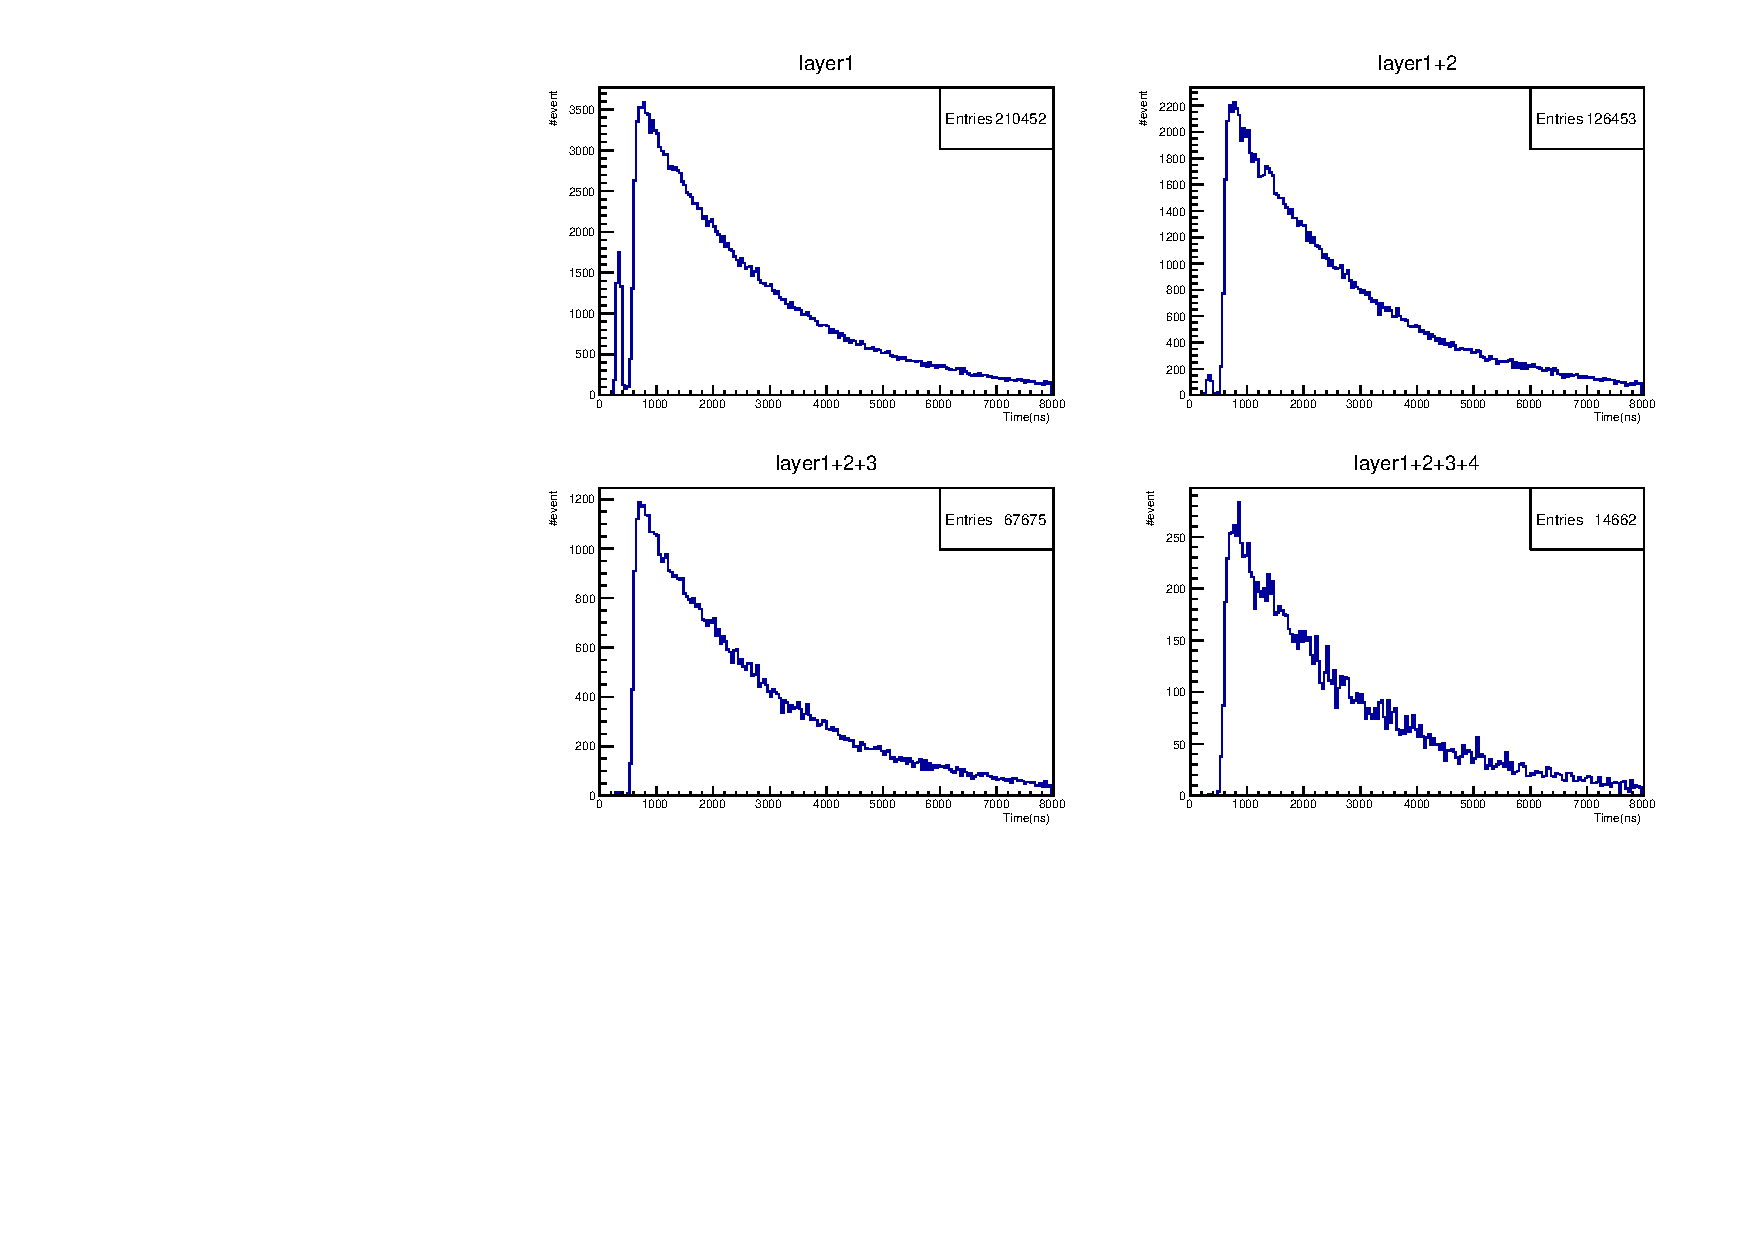
\includegraphics[height = 0.9\columnwidth , angle = -90]{figure/ikemitsu/lt_layercoin.pdf}
\caption{層でcoincidenceを取って得られたヒストグラム(磁場なし標的)}
\label{lt_layercoin}
\end{subfigure}
\begin{subfigure}{\columnwidth}
\centering
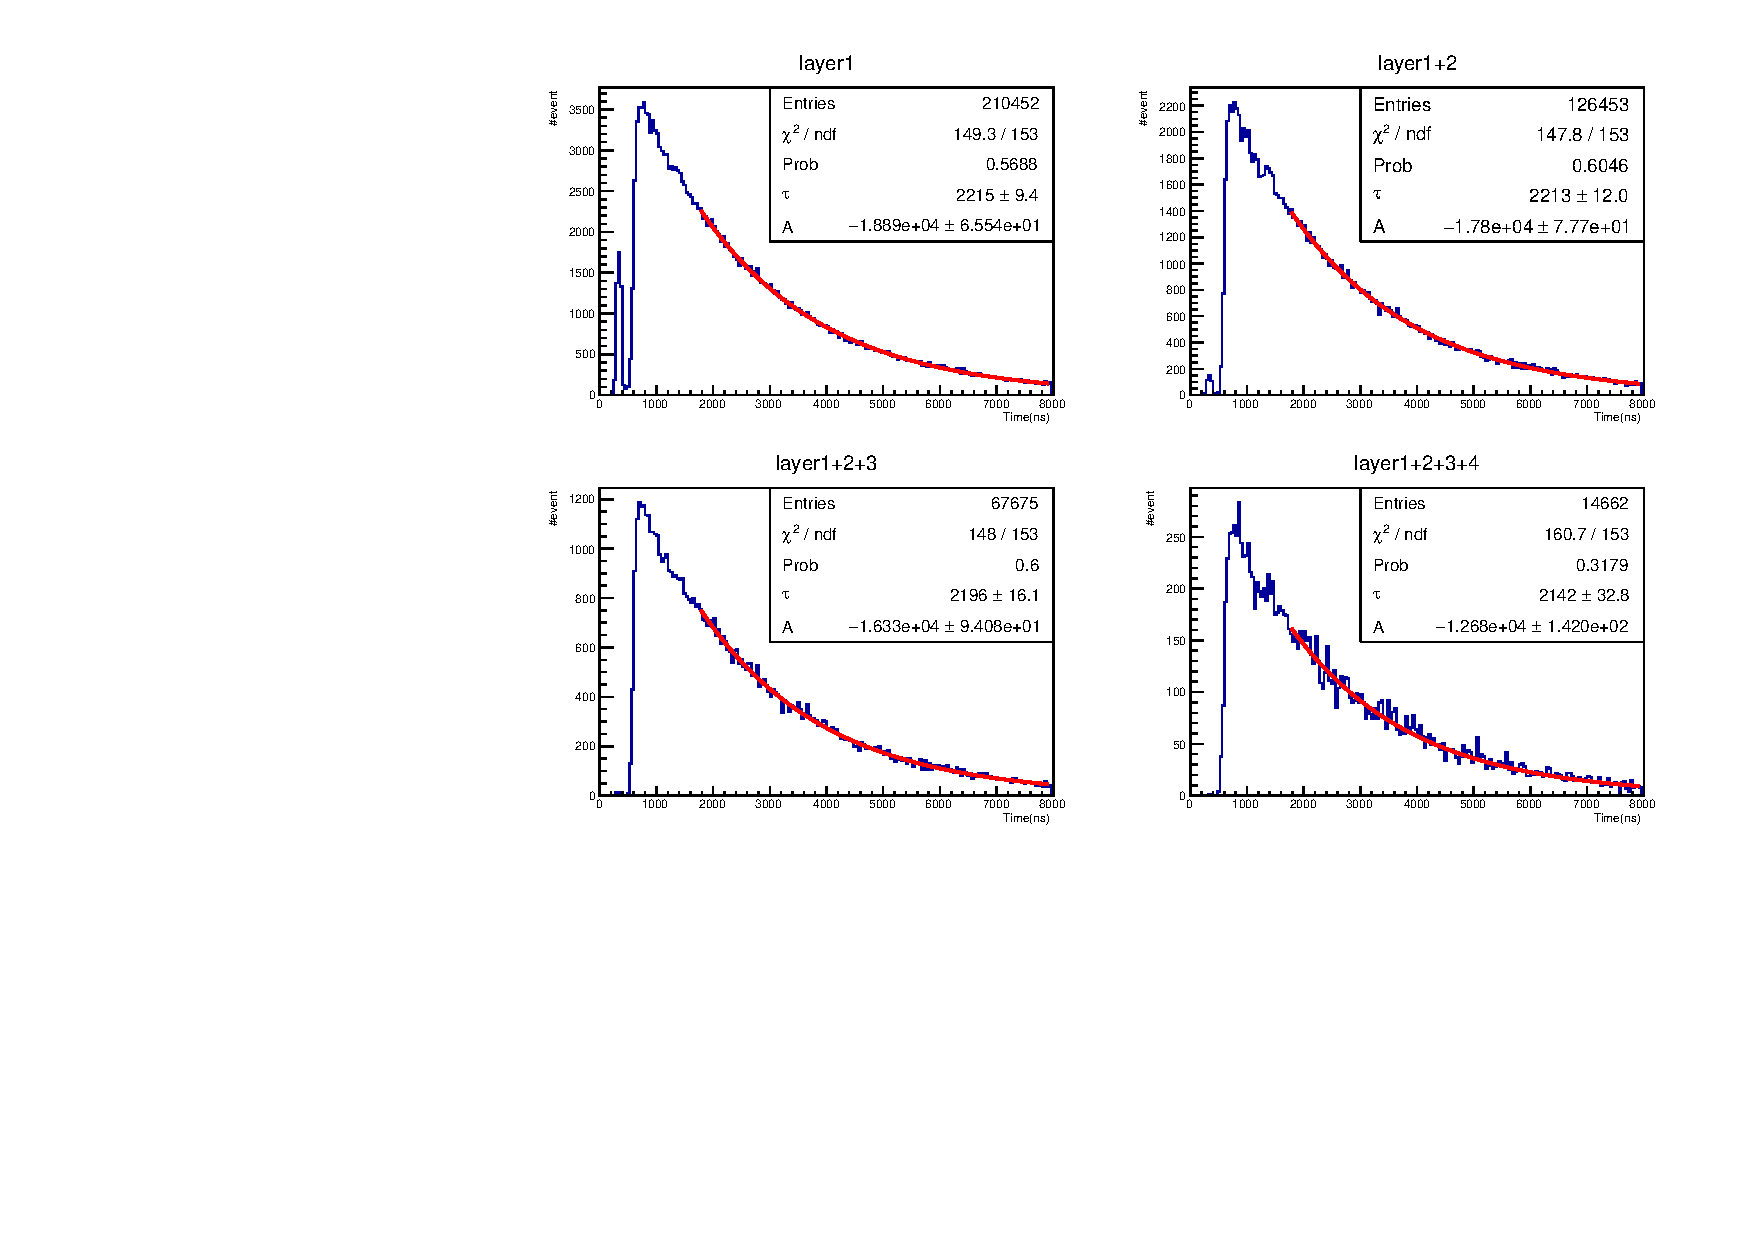
\includegraphics[height = 0.9\columnwidth , angle = -90]{figure/ikemitsu/lt_layercoin_fit.pdf}
\caption{$f_{\mathrm{life}}(t)$でfittingをした図}
\label{lt_layercoin_fit}
\end{subfigure}
\caption{fittingした図}
\label{lt_layercoin_all}
\end{figure}

\begin{figure}[H]
\centering
\begin{subfigure}{\columnwidth}
\centering
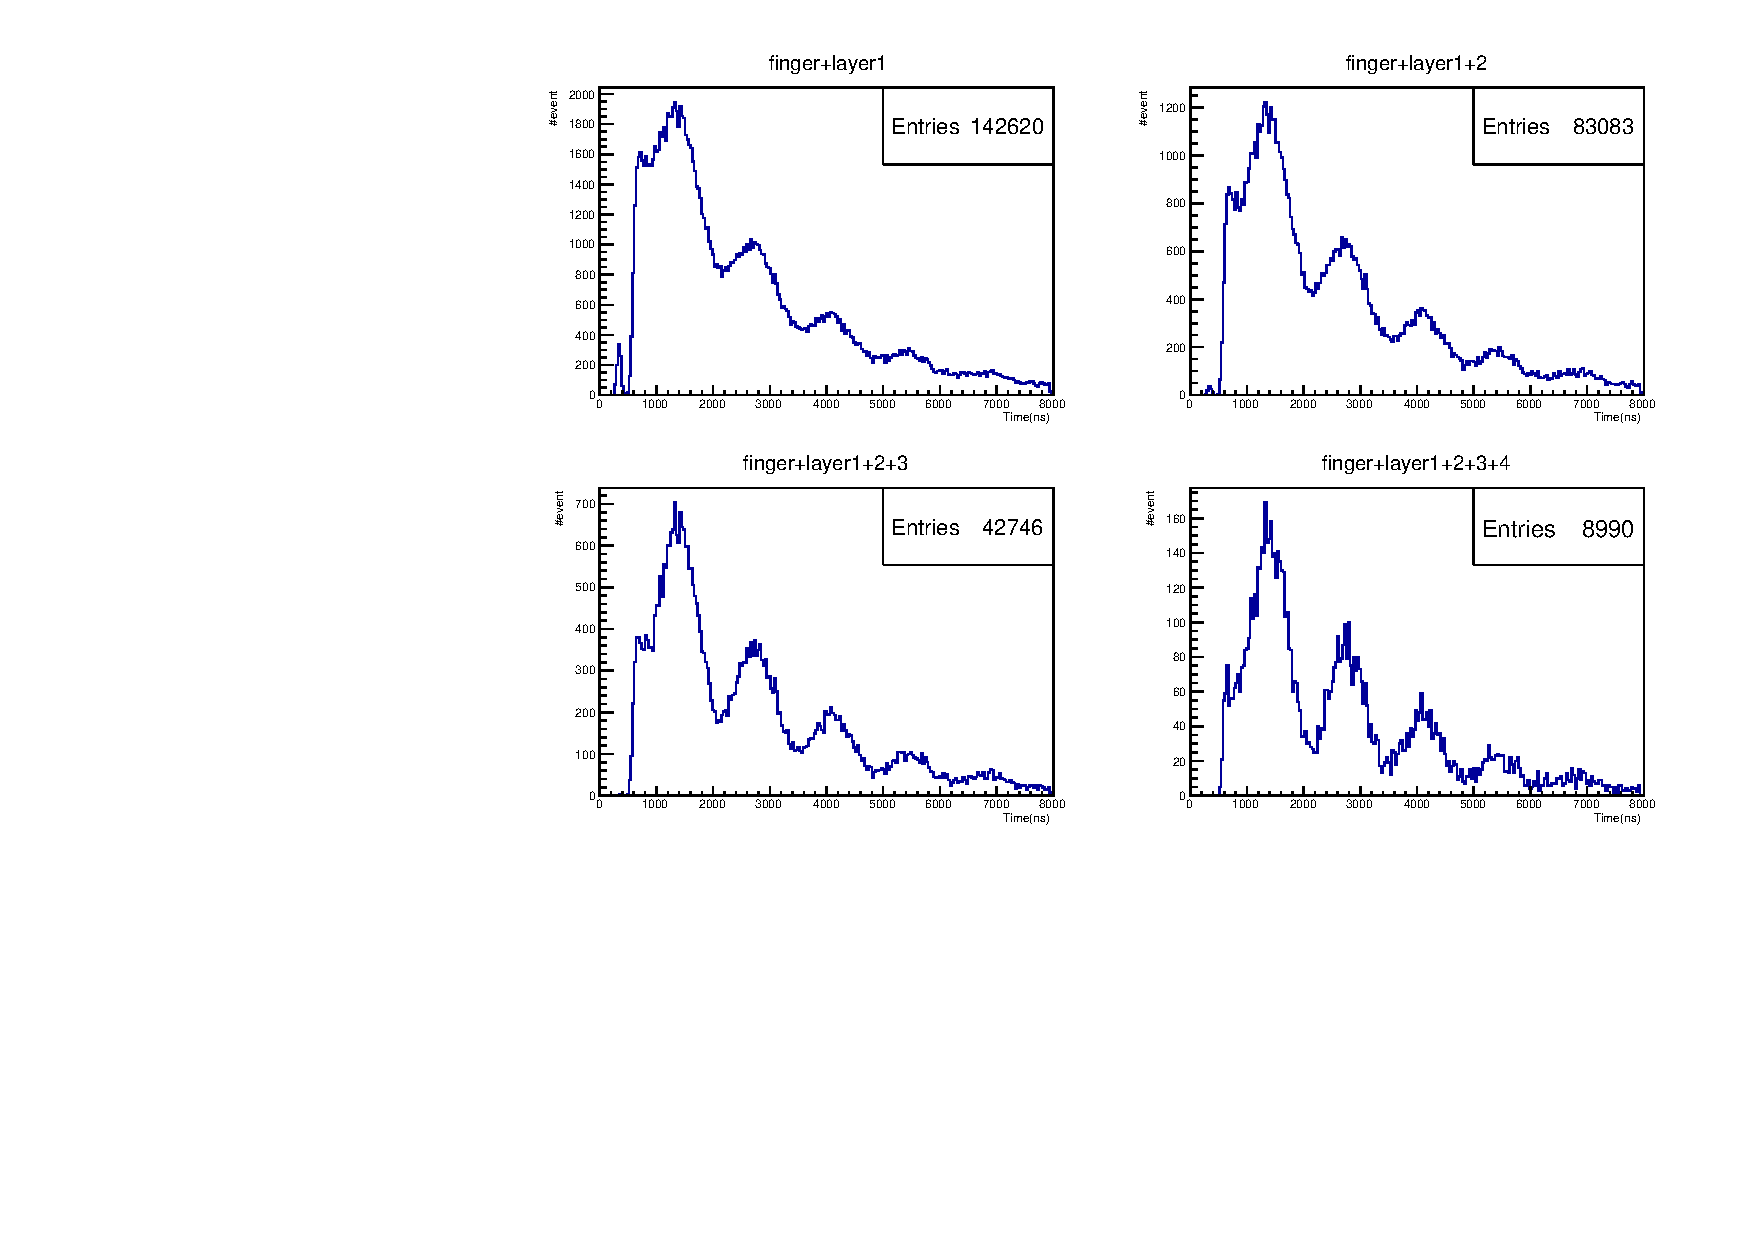
\includegraphics[height = 0.9\columnwidth , angle = -90]{figure/ikemitsu/g_layer_f_coin.pdf}
\caption{層でcoincidenceを取って得られたヒストグラム(磁場あり標的)}
\label{g_layercoin}
\end{subfigure}
\begin{subfigure}{\columnwidth}
\centering
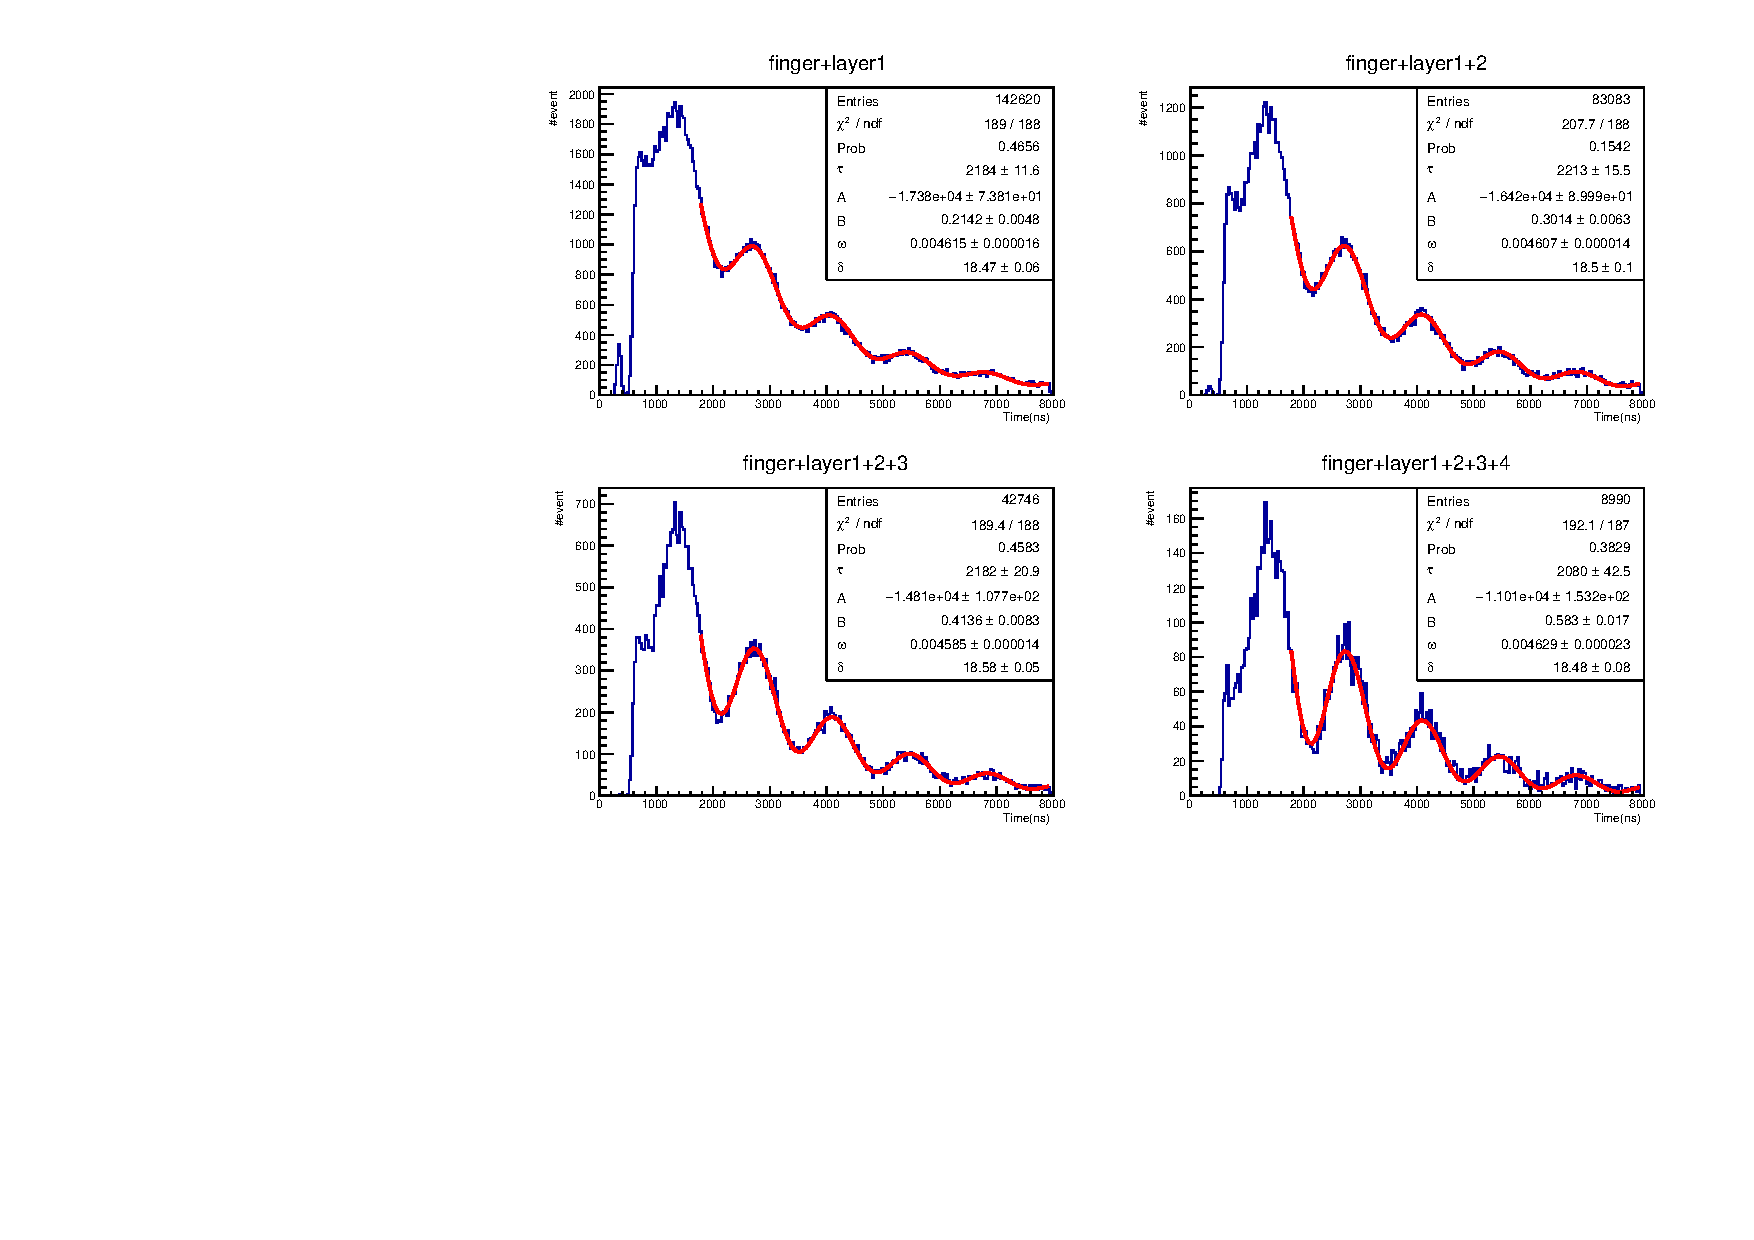
\includegraphics[height = 0.9\columnwidth , angle = -90]{figure/ikemitsu/g_laye_f_coin_fit.pdf}
\caption{$f_{g}(t)$でfittingをした図}
\label{g_layercoin_fit}
\end{subfigure}
\caption{fittingした図}
\label{g_layercoin_all}
\end{figure}

\subsubsection{エネルギー分布}
磁場なし標的を用いたときのデータから求めたエネルギー分布は図\ref{michel_PS}のようになった.
さらに,\ref{michel_PS}の各点において,キャリブレーションに由来するエネルギー分解能と統計誤差をそれぞれ横軸と縦軸の誤差として付けたのが図\ref{michel_PS_gosa}である.%図の縦軸の説明 2つの図で全然スケールが違うのはなぜ?
\begin{figure}[H]
\centering
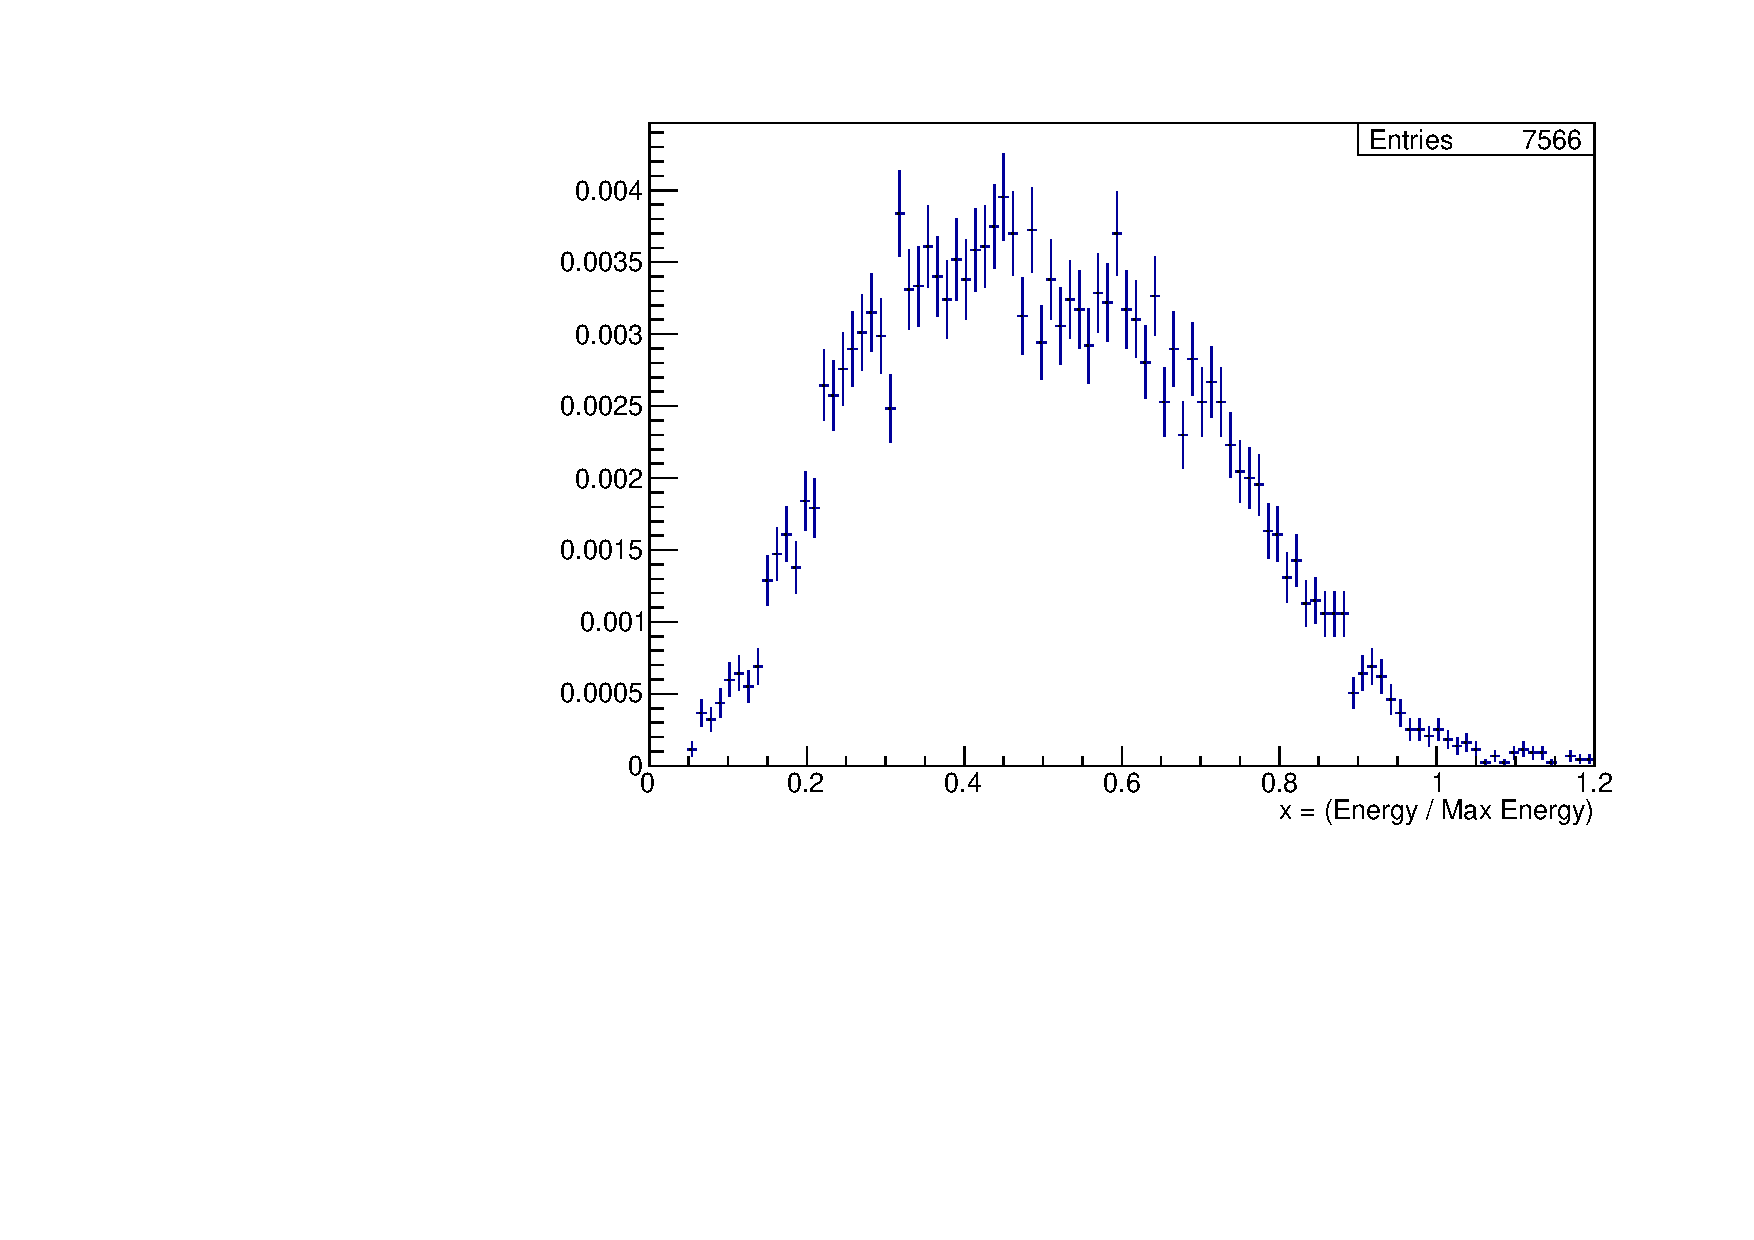
\includegraphics[height = 0.7\columnwidth , angle = -90]{figure/ikemitsu/michel_PS.pdf}
\caption{PSで得られたエネルギー分布図;磁場なし標的}
\label{michel_PS}
\end{figure}

\begin{figure}[H]
\centering
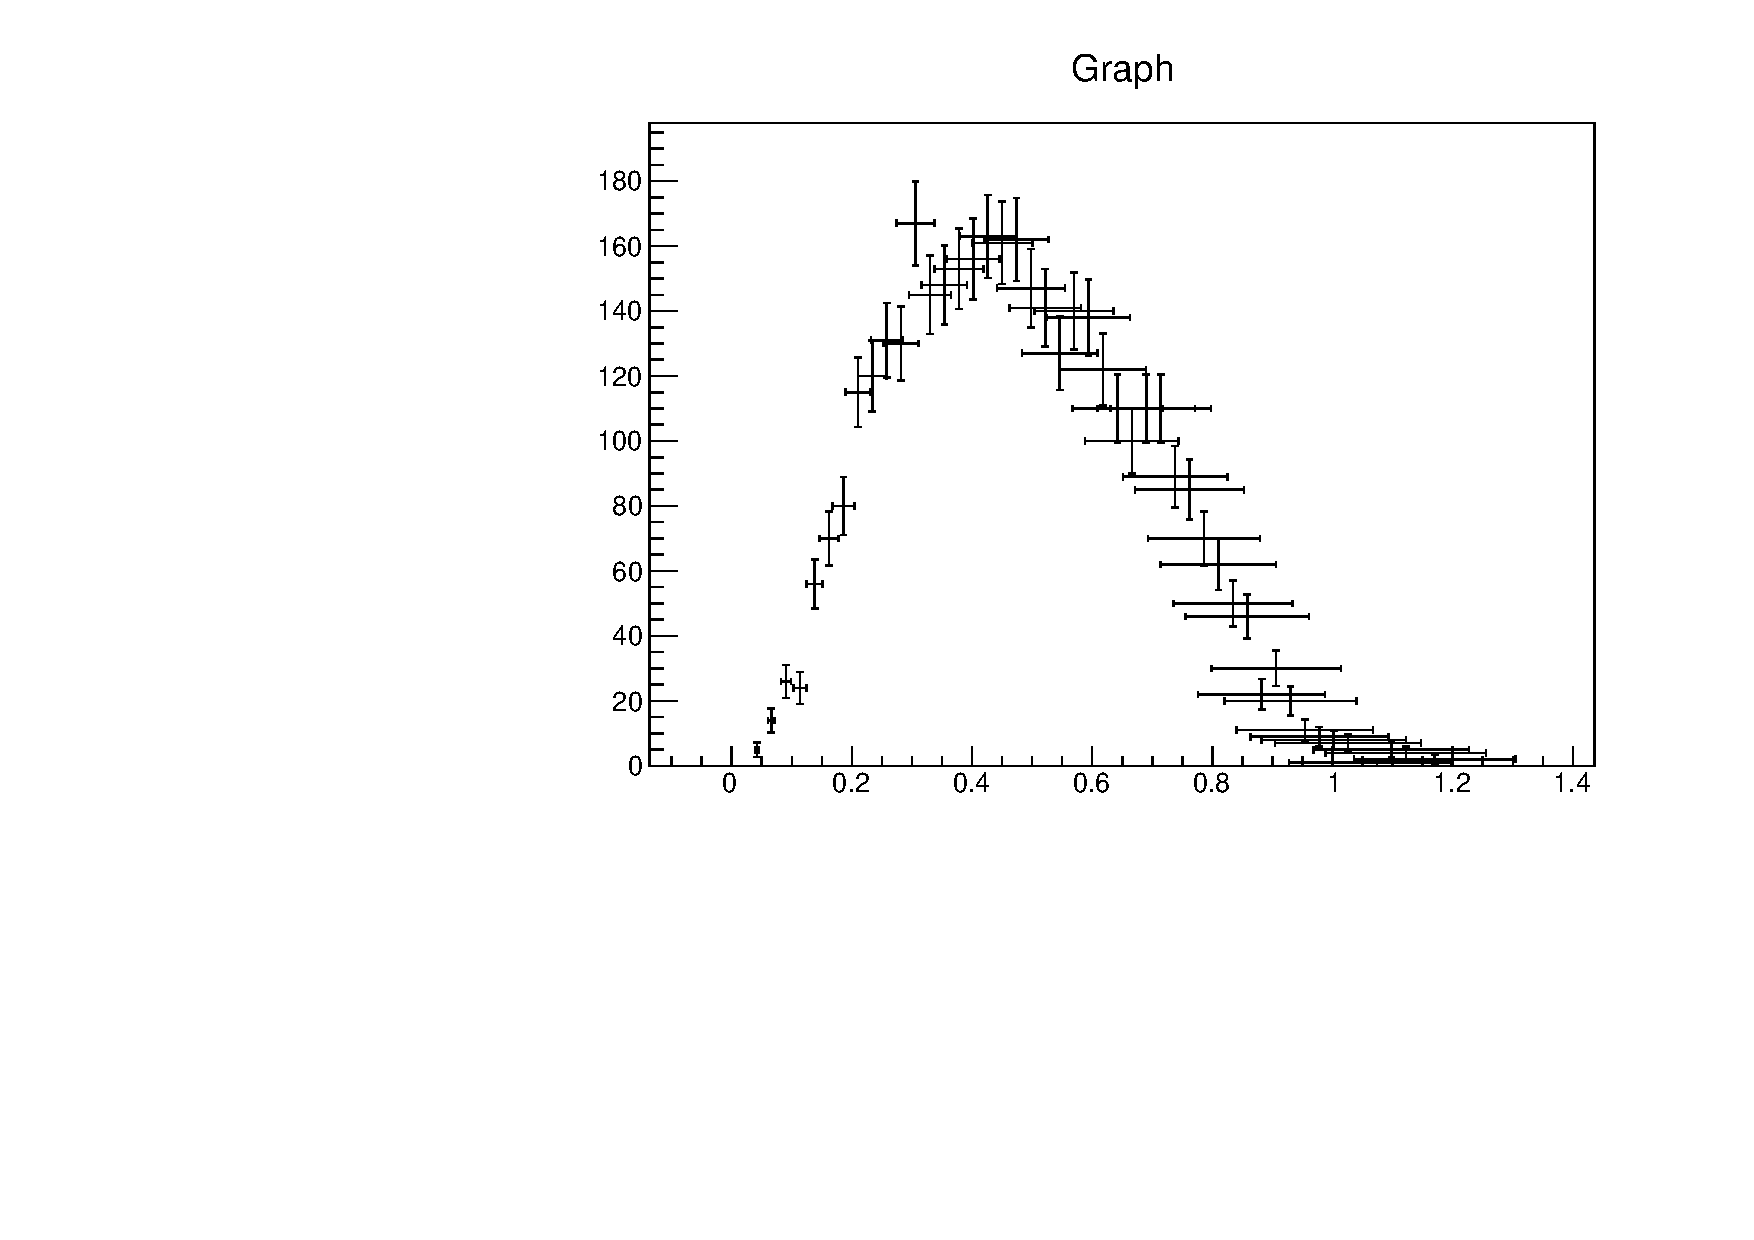
\includegraphics[height = 0.7\columnwidth , angle = -90]{figure/ikemitsu/michel_PS_gosa.pdf}
\caption{PSで得られたエネルギー分布(誤差付き);磁場なし標的}
\label{michel_PS_gosa}
\end{figure}

ミューオンのスピンに対して角度$\theta$の方向に崩壊する$\mathrm{e}^{+}$のエネルギー分布は,式\ref{eq:theory_michel}で与えられた.
この式に$\rho$以外のパラメータの値として,標準模型で予想されている$\eta = 0 , \xi = 1 , \xi \delta = 3/4$を代入して計算すると,
\begin{equation*}
\frac{d\Gamma}{dx} \propto x^{2} [\frac{2}{3}(\rho + \frac{3}{8}\cos \theta - \frac{1}{8})(4x-3) + \frac{1}{4}(\cos \theta + 3)]
\end{equation*}
となる。

図\ref{michel_PS_gosa}のグラフを$f_{\mathrm{michel}}(x) = x^{2} (A(4x -3) + B)$でfittingすることにより$\rho$を求めることができると考えた.
しかし,高エネルギー側での横軸の誤差が大きいこともありfittingはうまくいかなかった.以下ではエネルギー解析についての課題を述べる.

PSは無機シンチレータに比べて密度が小さいので,電磁シャワーで生じたフォトンが検出器の外側に漏れやすい.%フォトンの発生の頻度がNaIに比べて低いことも注目すべき
これによって高エネルギーの粒子の観測数が減ると考えられる.%観測数とはなにか?
解析的にこの課題を解決するには,シミュレーションによって入射粒子のエネルギーと観測されるエネルギーの対応を求めてfitting関数にその寄与を組み込む必要がある.%それでそれに対してどうするのか?

また,この実験ではPSのエネルギー較正に改善の余地が大いに残されている.
宇宙線ミューオンを用いたキャリブレーションならば,NaI検出器で行っているような,fingerとのcoincidenceをとることで精度を上げることができると考えられる.
% NaIではfingerとのcoincidenceをとるといった処理はしていない.事実誤認.

\subsubsection{fitting範囲による寿命と$g$因子の系統誤差}
今回使用したミューオンビームの分布は,FWHM$\sim$100 (ns) の幅を持ったガウス分布と考えることができる.
よって,図\ref{lt_layercoin}のヒストグラムのピーク点は750 (ns) であるが,その点から1000 (ns) はfittingの対象外とし,%なぜ1000ns?
図\ref{lt_layercoin_fit}と図\ref{g_layercoin_fit}ではfittingの範囲を1750 (ns) から7950 (ns) までとした.

この範囲の前側と後側で範囲を分けてfittingをすると,$\tau$と$g$の値は表\ref{fitrange1}〜\ref{fitrange4}のようになった.
\begin{table}[H]
\caption{寿命$\tau$;fitting範囲1750 (ns) 〜5250 (ns)}
\label{fitrange1}
\begin{center}
\begin{tabular}{cc}\toprule
coincidenceを取った層 	& $\tau$(ns) \\ \midrule
1 			& 2197 $\pm$ 16 \\
1+2 			& 2189 $\pm$ 20 \\
1+2+3 			& 2200 $\pm$ 28 \\
1+2+3+4 		& 2211 $\pm$ 60 \\ \bottomrule
\end{tabular}
\end{center}
\end{table}%

\begin{table}[H]
\caption{寿命$\tau$;fitting範囲4450 (ns) 〜7950 (ns)}
\label{fitrange2}
\begin{center}
\begin{tabular}{cc}\toprule
coincidenceを取った層 	& $\tau$(ns) \\ \midrule
1 			& 2247 $\pm$ 30 \\
1+2 			& 2244 $\pm$ 37 \\
1+2+3 			& 2218 $\pm$ 50 \\
1+2+3+4 		& 2036 $\pm$ 91 \\ \bottomrule
\end{tabular}
\end{center}
\end{table}%

\begin{table}[H]
\caption{$g$因子;fitting範囲1750 (ns) 〜5250 (ns)}
\label{fitrange3}
\begin{center}
\begin{tabular}{ccc}\toprule
coincidenceを取った層 	& $\omega$(/ns) 			& $g$ \\ \midrule
finger+1 		& $( 4.608 \pm 0.025 ) \times 10^{-3}$ 	& 2.004  $\pm$ 0.011 \\
finger+1+2 		& $( 4.585 \pm 0.023 ) \times 10^{-3}$ 	& 1.9938 $\pm$ 0.0098 \\
finger+1+2+3 		& $( 4.576 \pm 0.022 ) \times 10^{-3}$ 	& 1.9896 $\pm$ 0.0095 \\
finger+1+2+3+4 		& $( 4.615 \pm 0.032 ) \times 10^{-3}$ 	& 2.007  $\pm$ 0.014 \\ \bottomrule
\end{tabular}
\end{center}
\end{table}%

\begin{table}[H]
\caption{$g$因子;fitting範囲4450 (ns) 〜7950 (ns)}
\label{fitrange4}
\begin{center}
\begin{tabular}{ccc}\toprule
coincidenceを取った層 	& $\omega$(/ns) 			& $g$ \\ \midrule
finger+1 		& $( 4.570 \pm 0.060 ) \times 10^{-3}$ 	& 1.987 $\pm$ 0.024 \\
finger+1+2 		& $( 4.589 \pm 0.049 ) \times 10^{-3}$ 	& 1.995 $\pm$ 0.021 \\
finger+1+2+3 		& $( 4.579 \pm 0.049 ) \times 10^{-3}$ 	& 1.991 $\pm$ 0.021 \\
finger+1+2+3+4 		& $( 4.607 \pm 0.091 ) \times 10^{-3}$ 	& 2.003 $\pm$ 0.040 \\ \bottomrule
\end{tabular}
\end{center}
\end{table}%

これらの結果を表\ref{fit_lt},表\ref{fit_g}と比較すると,fittingの範囲を変えても,得られた$\tau$と$g$の値は誤差の範囲内で一致していると言える.
このことから,fittingの範囲として1750 ns から7950 ns までは適切だと考えられる.
%寿命に関して全層のcoincidenceがfittingの範囲が前半の時と後半の時とではコンシステントではない.系統誤差となるのでは?

しかし,寿命に関して表\ref{fitrange1}と表\ref{fitrange2}の1,2段目を比較すると,遅い時間側でfittingを行うと寿命が長くなっていると分かる.
これは,バックグラウンドなどのノイズを信号として処理しており,その影響がイベント数の少ない部分で強く出ていることによると考えることができる.
これを除くためには,より詳しい波形解析によってノイズとみなせる信号の性質を特定しなければならない.
今回の実験ではバックグラウンド計測をしなかったが,今後の課題として,ノイズ除去を目的とした解析を行う必要がある.
WFDを用いた実験では波形をデータとして残せるので,ノイズに起因する信号を取り除くことは可能だと考えられる.%どのようなノイズが想定されている?
寿命の解析結果として,表\ref{fit_lt}と表\ref{fitrange1}・表\ref{fitrange2}の違いをfitting範囲による系統誤差に含めた.%どのように?

$g$因子については,バックグラウンドがあっても振動の周期への影響はないと考えられる.%なぜ?
したがって,fitting範囲による系統誤差はないとした.

%%%%%%%%%%%%%%%%%%%池満パート終了%%%%%%%%%%%%%%%%%%%

%\end{document}

%\documentclass{jsarticle}

%\usepackage{amsmath, amssymb}%数式
%\usepackage{array, booktabs}%表成型
%\usepackage[dvipdfmx]{graphicx}%画像

%\begin{document}

\subsection{解析手法B}
\label{subsec:PSAnalyses}
% コインシデンス,フィッティングは他の節はアルファベット表記が多い
\subsubsection{使用データ}
\label{subsubsec:PSData}
実験で得られたデータのうち,解析に用いたのは3 日目に磁場標的を用いたランと4 日目に銅板標的を用いたランとの2 つであり,それぞれ表\ref{tab:PSdata} のようなデータであった.
\begin{table}[h]
	\centering
	\caption{PS の解析に用いたデータ}
	\begin{tabular}{ccc} \toprule
	標的の種類 & 磁場$B~(\mathrm{G})$ & Event 数 \\ \midrule
	銅板標的 & --- & 43502 \\
	磁場標的 & 53.97 & 448073 \\ \bottomrule
	\end{tabular}\label{tab:PSdata}
\end{table}%

なお,磁場標的を用いたデータについては先に述べたように磁場がランの途中で変化していたので,解析には変化後のデータとして,最初の30000 Event を除いたデータのみを用いた.
詳しくは\ref{subsubsec:PSMagChangeCheck}で述べる.

\subsubsection{WFD波形の解析}
\label{subsubsec:PSEventDisplay}
WFD (WaveDigitizer V1721) で得られたデータをプロットすると図\ref{fig:PSEventDisplayAll} のようになった.図\ref{fig:PSEventDisplayAll} は磁場標的を用いたランの1000 Event 目の波形であり,丸印はそれぞれの信号についてその点をピークとみなしたことを表す.ここでグラフの色はプラスチックシンチレータの各層に対応している(ただし3 層目にあたるch 4 はFinger Counter である).
%層の番号が標的から1,2,3,4となっている説明が前節までにない.?
\begin{figure}[h]
	\centering
	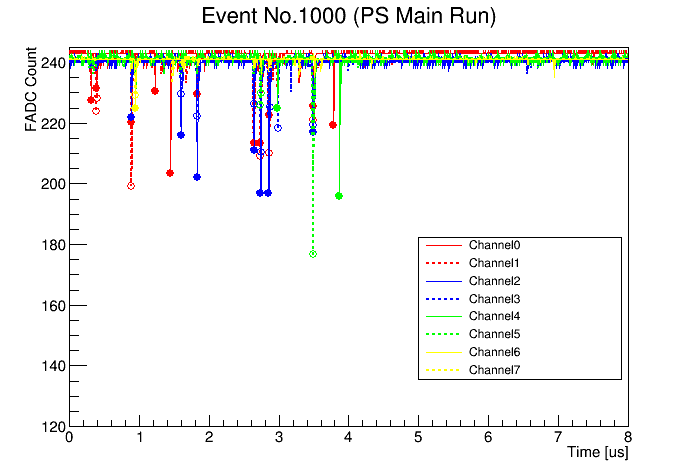
\includegraphics[width = 0.9\textwidth]{figure/odagawa/PSEventDisplayAll.png}
	\caption{プラスチックシンチレータで得られた波形($8~(\mu\mathrm{s})$ 全体)}
	\label{fig:PSEventDisplayAll}
\end{figure}%

図\ref{fig:PSEventDisplayAll} の$2.6~(\mu\mathrm{s})$ から$3.1~(\mu\mathrm{s})$ までを拡大したものが図\ref{fig:PSEventDisplayZoom} である.

\begin{figure}[h]
	\centering
	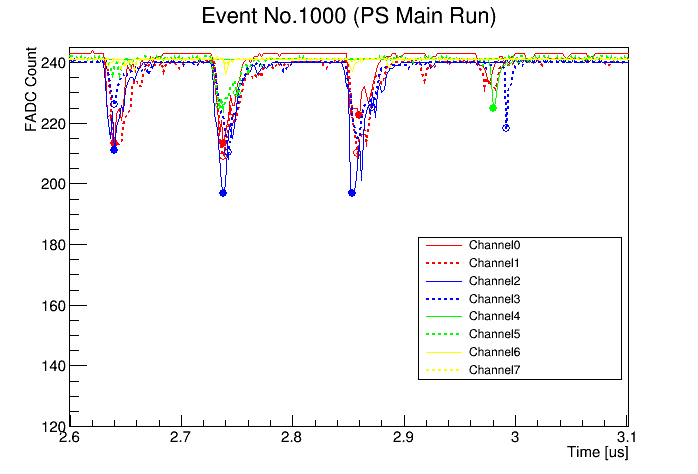
\includegraphics[width = 0.9\textwidth]{figure/odagawa/PSEventDisplayZoom.png}
	\caption{プラスチックシンチレータで得られた波形(一部拡大)}
	\label{fig:PSEventDisplayZoom}
\end{figure}%

図\ref{fig:PSEventDisplayZoom} からもわかる通り,プラスチックシンチレータの解析データについてはパイルアップの影響はほとんどないものと考えられる.また,信号の立ち上がりは十分早く,固定threshold 解析においてもTQ 補正などは必要ないと判断した.以降ではこれらを考慮したうえで,固定threshold を,プラスチックシンチレータのアフターパルスやベースラインの揺らぎを無視できる大きさ(8~WFD Count) に設定して解析を行った.

\subsubsection{ミューオン寿命解析}
\label{subsubsec:PSLife}
銅板標的を用いたランのデータの解析から,まずはミュオンの寿命を求めた.\ref{subsubsec:PSEventDisplay} で述べたようにthreshold を設定し,固定threshold を越えたところから初めて上回るところまでを一つの崩壊$e^{+}$ による信号として,threshold を超えた瞬間をその信号が持つ時間情報とした.その後,3 層目を除く各層については以下の方法でコインシデンスをとった.

各層について,時間情報が$10~(\mathrm{ns})$ 以内にあれば同じ崩壊$e^{+}$ 由来の信号として,二つの平均時間を各層の時間情報とした.ここで$10~(\mathrm{ns})$ という値は図\ref{fig:PSEventDisplayZoom} などからプラスチックシンチレータの立ち下がり時間程度になるように選んだ.

以上の時間情報を用いて実際に得られた3 層目を除く各層の時間情報ヒストグラムが図\ref{fig:PSLifeDist_Layer0} - \ref{fig:PSLifeDist_Layer3} である.ただし2, 4 層目は1 層目とのコインシデンスをとった.ここで3 層目を除いたのはチャンネル数の都合上,3 層目では層内でのコインシデンスをとることができなかったからである.また,コインシデンスをとった方法は各層での方法と同じであるが,時間情報としては1 層目と各層との平均を用いるのではなく,コインシデンスが取れたものを各層についてそのまま使用した.

\begin{figure}[h]
	\centering
	\begin{minipage}{0.45\textwidth}
	\centering
	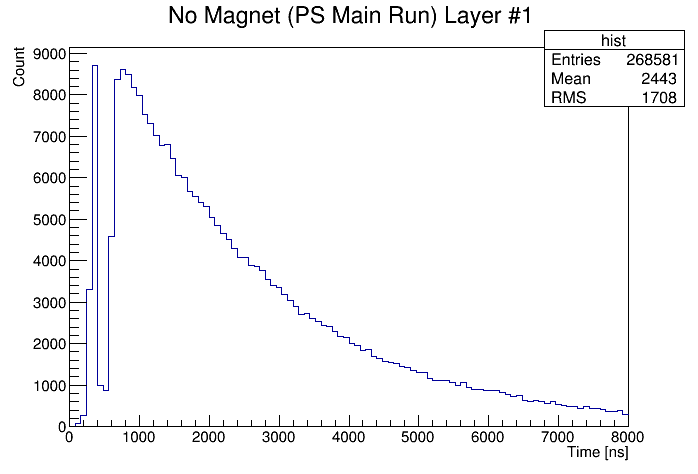
\includegraphics[width = \textwidth]{figure/odagawa/PSLifetimeDist_Layer0.png}
	\caption{磁場がないときの時間分布(1 層目)}
	\label{fig:PSLifeDist_Layer0}
	\end{minipage}
	\begin{minipage}{0.45\textwidth}
	\centering
	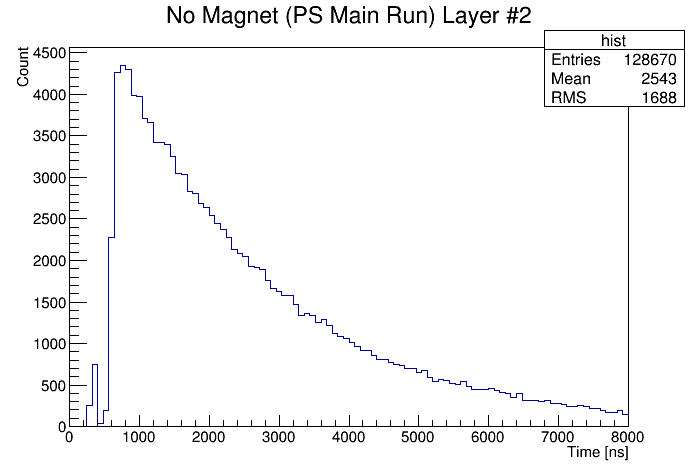
\includegraphics[width = \textwidth]{figure/odagawa/PSLifetimeDist_Layer1.png}
	\caption{磁場がないときの時間分布(2 層目)}
	\label{fig:PSLifeDist_Layer1}
	\end{minipage}
	\begin{minipage}{0.45\textwidth}
	\centering
	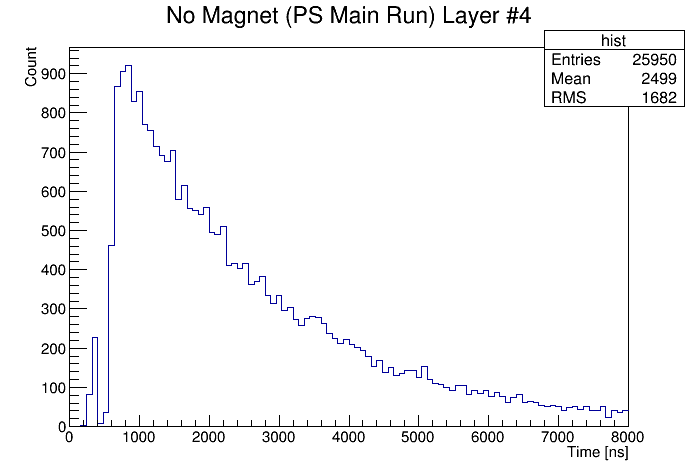
\includegraphics[width = \textwidth]{figure/odagawa/PSLifetimeDist_Layer3.png}
	\caption{磁場がないときの時間分布(4 層目)}
	\label{fig:PSLifeDist_Layer3}
	\end{minipage}
	\begin{minipage}{0.45\textwidth}
	\centering
	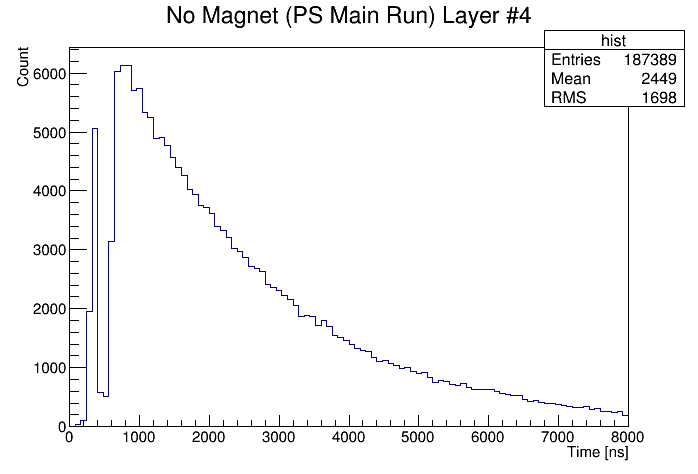
\includegraphics[width = \textwidth]{figure/odagawa/PSLifetimeDistNoCoin_Layer3.png}
	\caption{磁場がないときの時間分布(4 層目,コインシデンスなし)}
	\label{fig:PSLifeDistNoCoin_Layer3}
	\end{minipage}
\end{figure}%

得られた時間分布について,まず早いところにピークが立っている.このピークは図\ref{fig:PSLifeDist_Layer3}, \ref{fig:PSLifeDistNoCoin_Layer3} を比較すると分かるように,コインシデンスをとることによって小さくなる.このピークは$\pi$ の崩壊によってできた表面ミュオンがすぐに崩壊し,生成した$e^{+}$ が,ビームラインを通り抜けて直接検出器に当たったときの信号によるものと考えられる.ビームラインにおいては運動量で粒子を選択しており(今回は$4.1~(\mathrm{MeV})$ の粒子を選択している),このようにしてできた$e^{+}$は同じ運動量の$\mu^{+}$ よりも高速で検出器に到達する.1 層目とのコインシデンスをとることでこのピークが低くなるのは,このコインシデンスにより粒子の飛来した方向を制限でき,銅板標的由来の信号の割合が多くなるためと考えられる.

図\ref{fig:PSLifeDist_Layer0} - \ref{fig:PSLifeDist_Layer3} のヒストグラムに式\eqref{eq:PSLifeFitFunc} で表される関数$f(t)$を用いてフィッティングを行った.ここでバックグラウンドの影響を加味して定数項を加え,フィッテイング範囲は1000~(ns) から8000~(ns) とした.フィッティング結果が図\ref{fig:PSLifeFit_Layer0} - \ref{fig:PSLifeFit_Layer3} ,および表\ref{tab:PSLifetime} である.統計誤差はROOT のフィッティングによるものである.
% ミューオンの4層目の値は外れ値?
% 最終的なミューオンの寿命の解析の値は?
\begin{equation}
f(t) = A \exp(-t / \tau) + \mathrm{const.}
\label{eq:PSLifeFitFunc}
\end{equation}

\begin{figure}[h]
	\centering
	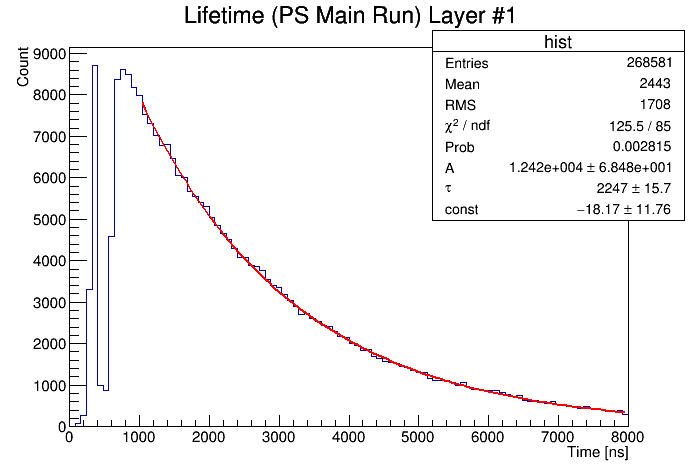
\includegraphics[width = 0.45\textwidth]{figure/odagawa/PSLifetimeFit_Layer0.png}
	\caption{ミューオン崩壊寿命フィッティング結果(1 層目)}
	\label{fig:PSLifeFit_Layer0}
	\begin{minipage}{0.45\textwidth}
	\centering
	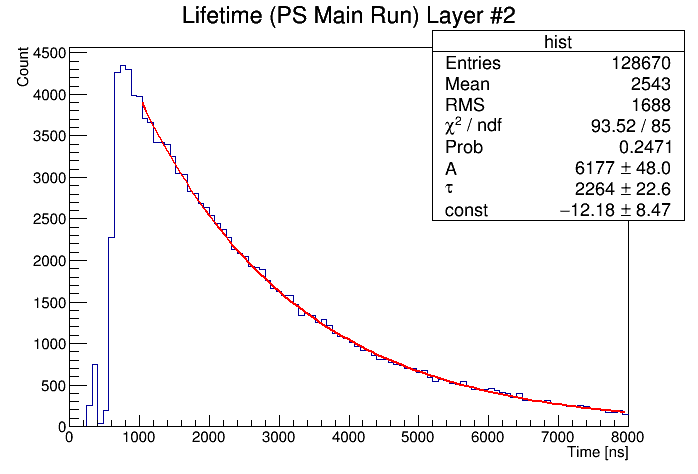
\includegraphics[width = \textwidth]{figure/odagawa/PSLifetimeFit_Layer1.png}
	\caption{ミューオン崩壊寿命フィッティング結果(2 層目)}
	\label{fig:PSLifeFit_Layer1}
	\end{minipage}
	\begin{minipage}{0.45\textwidth}
	\centering
	\includegraphics[width = \textwidth]{figure/odagawa/PSLifetimeFit_Layer3.png}
	\caption{ミューオン崩壊寿命フィッティング結果(4 層目)}
	\label{fig:PSLifeFit_Layer3}
	\end{minipage}
\end{figure}%

\begin{table}[h]
	\centering
	\caption{フィッティングによって得られた$\tau$ の値}
	\begin{tabular}{cc}\toprule
	層番号 & $\tau~[\mathrm{ns}]$ \\ \midrule
	1 & $2247 \pm 16$ \\
	2 & $2264 \pm 23$ \\
	4 & $2150 \pm 46$ \\ \bottomrule
	\end{tabular}\label{tab:PSLifetime}
\end{table}%

\newpage

\subsubsection{ミューオン$g$ 因子解析}
\label{subsubsec:PSgFactor}
次に磁場標的を用いたランの解析から,ミューオンの$g$ 因子を求めた.ここで先述の通り,磁場の変化を確認した結果から,最初の30000~Events を除いたデータを用いた.\ref{subsubsec:PSLife} と同様に時間情報を求めて図\ref{fig:PSgFactorDist_Layer0} - \ref{fig:PSgFactorDist_Layer3} のようなヒストグラムを得た.

\begin{figure}[h]
	\centering
	\includegraphics[width = 0.45\textwidth]{figure/odagawa/PSgFactorDist_Layer0.png}
	\caption{磁場があるときの時間分布(1 層目)}
	\label{fig:PSgFactorDist_Layer0}
	\begin{minipage}{0.45\textwidth}
	\centering
	\includegraphics[width = \textwidth]{figure/odagawa/PSgFactorDist_Layer1.png}
	\caption{磁場があるときの時間分布(2 層目)}
	\label{fig:PSgFactorDist_Layer1}
	\end{minipage}
	\begin{minipage}{0.45\textwidth}
	\centering
	\includegraphics[width = \textwidth]{figure/odagawa/PSgFactorDist_Layer3.png}
	\caption{磁場がないときの時間分布(4 層目)}
	\label{fig:PSgFactorDist_Layer3}
	\end{minipage}
\end{figure}%

図\ref{fig:PSgFactorDist_Layer0} - \ref{fig:PSgFactorDist_Layer3} のヒストグラムに式\eqref{eq:PSgFactorFitFunc} で表される関数$g(t)$ を用いてフィッティングを行った.ここで\ref{subsubsec:PSLife} のときと同様に定数項を加え,フィッティング範囲も振動がきちんと見えている1000~ns から8000~ns までとした.フィッティング結果は図\ref{fig:PSgFactorFit_Layer0} - \ref{fig:PSgFactorFit_Layer3},および表\ref{tab:PSgFactor} となった.ただし表\ref{tab:PSgFactor} において$g$ 因子の計算には各点の磁場をビームプロファイルのガウシアンで加重平均した値,$B = 53.97~(\mathrm{G})$ という値を用いた.また,統計誤差としては\ref{subsubsec:PSLife} と同様にROOT のフィッティングによって得られたものを載せており,磁場の影響を含めたものについては後述する.

\begin{equation}
g(t) = A \exp(-t / \tau) [1 + B \cos(\delta + \omega t)] + \mathrm{const.}
\label{eq:PSgFactorFitFunc}
\end{equation}

\begin{figure}[h]
	\centering
	\includegraphics[width = 0.45\textwidth]{figure/odagawa/PSgFactorFit_Layer0.png}
	\caption{ミューオン$g$ 因子フィッティング結果(1 層目)}
	\label{fig:PSgFactorFit_Layer0}
	\begin{minipage}{0.45\textwidth}
	\centering
	\includegraphics[width = \textwidth]{figure/odagawa/PSgFactorFit_Layer1.png}
	\caption{ミューオン$g$ 因子フィッティング結果(2 層目)}
	\label{fig:PSgFactorFit_Layer1}
	\end{minipage}
	\begin{minipage}{0.45\textwidth}
	\centering
	\includegraphics[width = \textwidth]{figure/odagawa/PSgFactorFit_Layer3.png}
	\caption{ミューオン$g$ 因子フィッティング結果(4 層目)}
	\label{fig:PSgFactorFit_Layer3}
	\end{minipage}
\end{figure}%

\begin{table}[h]
	\centering
	\caption{$g$ 因子フィッティング結果}
	\begin{tabular}{cccc} \toprule
	層番号 & $\tau~[\mathrm{ns}]$ & $\omega~[/ \mu\mathrm{s}]$ & $g$ \\ \midrule
	1 & $2249 \pm \phantom{0}4$ & $4.624 \pm 0.004$ & $2.013 \pm 0.0015$ \\  
	2 & $2224 \pm \phantom{0}6$ & $4.620 \pm 0.003$ & $2.012 \pm 0.0015$ \\  
	4 & $2066 \pm 13$ & $4.633 \pm 0.005$ & $2.017 \pm 0.0023$ \\  \bottomrule
	\end{tabular}\label{tab:PSgFactor}
\end{table}%

\newpage

\subsubsection{磁場の系統誤差について}
\label{subsubsec:MagSysErr}
\ref{subsubsec:PSgFactor} において$g$ 因子解析に用いた磁場の値$B = 53.97~[\mathrm{Gauss}]$ は事前にMLF の三宅さんから頂いたビームプロファイルをもとに加重平均をとった値であるが,このビームプロファイルの不定性により加重平均の値は変化する.今回はビームの広がりはガウシアンに乗ると仮定したうえでガウシアンの広がりを変化させ,それによって現れる磁場,および$g$ 因子の系統誤差をみた.

ガウシアンの$x$ 方向の広がりを$\sigma_{x}$,$y$ 方向の広がりを$\sigma_{y}$ とし,$\sigma_{x}$ を2.0~cm から3.9 ~cm まで,$\sigma_{y}$ を1.0~cm から2.9~cm まで0.1~cm 刻みで変化させて加重平均磁場の値を求めたところ磁場の最大値・最小値は表\ref{tab:MagSysErr} のようになった.ここで$\sigma_{x}, \sigma_{y}$ を動かす範囲は磁場標的の大きさが標準偏差$1\sigma$ に入る点を上限として十分な広さをとった.

\begin{table}[h]
	\centering
	\caption{$\sigma_{x}$,$\sigma_{y}$を動かしたときの磁場$B$ の最大値と最小値~(G)}
	\begin{tabular}{cc}\toprule
	$B_{\mathrm{max}}$ & $B_{\mathrm{min}}$ \\ \midrule
	$54.44 (\sigma_{x} = 3.9, \;\sigma_{y} = 1.0)$ & $53.76 (\sigma_{x} = 3.9,\;\sigma_{y} = 2.9)$ \\ \bottomrule 	
	\end{tabular}\label{tab:MagSysErr}
\end{table}%

得られた磁場の最大値,および最小値を用いて$g$ 因子を計算すると表\ref{tab:PSgSysErr} のような値がそれぞれ得られた.

\begin{table}[h]
	\centering
	\caption{磁場$B$ の値とそれらに対応する$g$ 因子の値}
	\begin{tabular}{cccc}\toprule
	層番号 & $B_{\mathrm{max}} = 54.44$ & $B_{0} = 53.97$ & $B_{\mathrm{min}} = 53.76$ \\ \midrule
	1 & 2.000 & 2.013 & 2.021 \\
	2 & 1.995 & 2.012 & 2.020 \\
	4 & 2.000 & 2.017 & 2.025 \\ \bottomrule 
	\end{tabular}\label{tab:PSgSysErr}
\end{table}%

また,磁場の測定誤差を含んだ$g$ 因子の統計誤差については,誤差伝播の式,式\eqref{eq:PSgosa} を用いて計算した.$\delta B = 0.008~(\mathrm{G})$となったので,$\delta g$ は表\ref{tab:PSgStatErr} のようになった.

\begin{equation}
\delta g = \sqrt{\left(\delta\omega\right)^{2}\left(\frac{\partial g}{\partial\omega}\right)^{2} + \left(\delta B\right)^{2}\left(\frac{\partial g}{\partial B}\right)^{2}}
\label{eq:PSgosa}
\end{equation}%

\begin{table}
	\centering
	\caption{磁場の測定誤差を含んだ$g$ 因子の統計誤差}
	\begin{tabular}{cc}\toprule
	層番号 & $g$ 因子の統計誤差\\ \midrule
	1 & 0.0016 \\ 
	2 & 0.0015 \\
	4 & 0.0023 \\ \bottomrule
	\end{tabular}\label{tab:PSgStatErr}
\end{table}%

実際,$g$ 因子の値を考えるときは1 層目と4 層目とのコインシデンスをとったものが貫通イベントをとれている可能性が高く妥当であると考えると,得られた$g$ 因子の値は
% 貫通イベントはどのようなイベントが多いから妥当?
\[g = 2.017 \pm 0.0023 ^{+0.008}_{-0.017}\]
となった.ここで誤差の第一項は磁場の影響を含めた統計誤差であり,第二項はビームプロフィルの不定性による系統誤差である.

%以下二つはAppendix にまわす?
%%%%%%%%%%%%%%%
\subsubsection{磁場の変化の確認}
\label{subsubsec:PSMagChangeCheck}
$g$ 因子測定のための磁場標的を置いたランの途中において磁石配置が崩れ,磁場の値などが変わっていたことは本文中でも述べたが解析においてそのことを確認した.

\ref{subsubsec:PSgFactor} のようなフィッティングをする際に,用いるイベントを9000~Events (6~min) ごとに区切ってフィッティングを行い,それぞれ$\omega$ を求めると図\ref{fig:PSOmegaCheck} のようになった.また図\ref{fig:PSCycleCheck} はそれぞれを振動周期に直したものである.赤線は最初の8~分間のデータのみがたまたまあったのでそこから得られた値を表しており,また青線は磁場変化発覚後に改めて確認用にとったランから得られた値を表している.図\ref{fig:PSOmegaCheck}, \ref{fig:PSCycleCheck} を見ると分かるように,ランの最初の20~分程度で磁場の値が変化していることが分かる.よって今回の解析には同じ値の磁場とみなせるという条件の下で,より統計量の多いランの20~分以降のデータを用いることにした.なお,変化前後の加重平均をとった磁場の値はそれぞれ56.06~(G) と53.97 (G) であった.

\begin{figure}[h]
	\centering
	\begin{minipage}{0.45\textwidth}
	\centering
	\includegraphics[width = \textwidth]{figure/odagawa/PSOmegaCheck.png}
	\caption{ラン中における$\omega$ の時間変化}
	\label{fig:PSOmegaCheck}
	\end{minipage}
	\begin{minipage}{0.45\textwidth}
	\centering
	\includegraphics[width = \textwidth]{figure/odagawa/PSCycleCheck.png}
	\caption{ラン中における振動周期 の時間変化}
	\label{fig:PSCycleCheck}
	\end{minipage}
\end{figure}

\subsubsection{NaI シンチレータとの位相差の確認}
\label{subsubsec:PhaseCheck}
NaI シンチレータとプラスチックシンチレータの$g$ 因子の解析から$\cos$ 振動の初期位相$\delta$ に注目すると,これら二つの位相差は実験中の物理的セットアップに起因していると考えられる.実際,二つのシンチレータは標的に対しておよそ$87^{\circ}$ の角度をつけて配置していたため,それにともなって初期位相もおよそ$87^{\circ}$ 分の差をもっているはずである.

これらの事実を解析から確かめるために,まず二つの検出器から得られたデータの時間原点をそろえる必要がある.これら二つの検出器では検出器の性能差もあるが,そもそも信号の伝送に用いたケーブルの長さが違うために時間原点がそろっていない.今回は時間原点をそろえるために\ref{subsubsec:PSLife} でものべた高速$e^{+}$ 粒子による小さなピークでそろえることを考えた.ビームライン奥からミュオンに比べて高速で飛んでくる$e^{+}$ は,今回のセットアップにおいては二つの検出器にほぼ同様の時間かけて飛んでくるはずなので,このピークをそろえることで時間原点とすることができる.図\ref{fig:NaITimeOrigin}がNaI シンチレータの$e^{+}$ ピーク探索とそれを用いた原点調整後のヒストグラム,図\ref{fig:PSTimeOrigin} はプラスチックシンチレータで同様のことを行ったものである.

\begin{figure}[h]
	\centering
	\includegraphics[width = 0.9\textwidth]{figure/odagawa/NaITimeOrigin.png}
	\caption{NaI シンチレータにおける時間原点探索と原点調節後のヒストグラム}
	\label{fig:NaITimeOrigin}
	\includegraphics[width = 0.9\textwidth]{figure/odagawa/PSTimeOrigin.png}
	\caption{プラスチックシンチレータにおける時間原点探索と原点調節後のヒストグラム}
	\label{fig:PSTimeOrigin}
\end{figure}

それぞれのフィッティングから得られた初期位相$\delta$ は表\ref{tab:InitPhases} のようになった.

\begin{table}[h]
	\centering
	\caption{各検出器の初期位相}
	\begin{tabular}{cc}\toprule
	検出器 & $\delta$ \\ \midrule
	NaI シンチレータ & $-0.54 \pm 0.04$ \\
	プラスチックシンチレータ & $\phantom{-}1.10 \pm 0.02$ \\ \bottomrule
	\end{tabular}\label{tab:InitPhases}
\end{table}%
したがって,表\ref{tab:InitPhases} からもわかるとおり位相差は$1.64 \pm 0.06 \sim \pi / 2$ となりセットアップの角度と整合していることが確認できた.

\subsection{解析まとめ}
% 以下,解析手法Aの結果のコピペ
解析の結果得られたミューオンの寿命と$g$因子の値は表\ref{matome_ike}のようになった。寿命の誤差は統計誤差とfitting範囲による系統誤差で、$g$因子の誤差は統計誤差である。

\begin{table}[H]
\caption{解析結果}
\label{matome_ike}
\begin{center}
\begin{tabular}{cc}\toprule
$\tau$(ns) 	& 2212 $\pm$ 12 $^{ + 35}_{ - 15}$  \\ \midrule
$g$		& 2.003 $\pm$ 0.006 \\ \bottomrule
\end{tabular}
\end{center}
\end{table}%

%%%%%%%%%%%%%%%
%\end{document}

%\usepackage{here}
%\usepackage[dvipdfmx]{graphicx}
%\usepackage{amsmath,amssymb}
%\usepackage{array,booktabs} %表のためのarray環境

%\begin{document}
\section{NaIで取得したデータの解析と結果・考察}
以下では主に測定した信号から欲しい情報を取り出すための解析に関する部分と,得られた情報から実際の測定した量を解析する部分にわけて,解析の詳細を述べる.
特に前半の信号解析ではパイルアップ信号を取り除く処理を行い,情報を取り出す解析を行った.
後半では寿命と$g$ 因子の測定をフィッティングを用いて行った.
また,ミッシェルパラメータの測定では時間情報に基づいたスピンの情報とエネルギーの相関を含めた解析を行った.
その際,各NaIで得られたエネルギー情報に対し測定器の電磁シャワーの応答に基づくフィッティングを行った.

\subsection{信号解析}
NaI 検出器で測定した波形解析の手法について述べる.
測定波形の中で典型的なものを\figref{hatano_fig:rawdata} に示す.
波形解析ではここからフィンガーカウンター(チャンネル1 )が鳴っているという条件を課したときにNaI で測定したエネルギーと信号の時刻という2 つの情報を抽出した.
この際に信号のノイズとNaI と波形の重なり(以下,パイルアップとよぶ)の2 つが解析時の注意点となった.
前者は信号が鳴ったという判定をするためのピーク検出をする際に問題となる.
具体的には,本来1 つの$e^+$ からの信号であるのにノイズの影響で複数のピークとして認識してしまう.
そのため,今回の解析ではノイズ除去の処理を最初に行った.
その後ピーク検出を行った後に時間情報とエネルギー情報を取り出す.
この際にパイルアップの処理をしないまま適当な領域で積分を行いエネルギーを求めると,別の$e^+$ からの信号でエネルギーが大きく見積もられてしまう.
このため,今回の解析では波形データのサンプリングを行い,それに基づきパイルアップしてない部分の波形からパイルアップしている部分に外挿し,その分の補正を行った.
以下具体的な処理について述べる.

\begin{figure}[hbt]
\centering
\includegraphics[width=0.6\textwidth]{figure/hatano/rawdata_modify1.eps}
\caption{NaI 検出器の測定信号.チャンネル1 はフィンガーカウンターの測定波形,チャンネル3 〜チャンネル7 はNaI の測定波形.NaIの測定波形では波形の重なりが見られる.}
\label{hatano_fig:rawdata}
\end{figure}

\subsubsection{ノイズ除去}
ピーク検出の際に問題となる高周波のノイズを除去することについて考える.
高周波成分によるピークと誤認識するような大きな変動がなくなればいいので,簡単に実装ができかつ高速な処理ができるという観点で単純移動平均をとるということを行った.
具体的には各サンプリング点で前後4 サンプリング,計9 サンプリングの平均をとった.
実際にノイズ除去を行った前後の信号の差異は\figref{hatano_fig:smoothdata}(\figref{hatano_fig:smoothdata} と同じデータの一部)のようになった.
チャンネル6 の左側の信号はノイズによって2 つのピークのように見かけ上分裂していたのが改善しているのが分かる.

\begin{figure}[hbt]
\centering
\includegraphics[width=0.6\textwidth]{figure/hatano/smoothdata_modify1.eps}
\caption{ノイズ除去された測定信号.薄い色で示したのが元の信号,濃い色で示したのがノイズ除去を行った信号.チャンネル6 の信号はノイズによって2 つのピークのように見かけ上分裂していたのが改善している.}
\label{hatano_fig:smoothdata}
\end{figure}

\subsubsection{ピーク検出}
以上のノイズ除去を行った信号を元にピーク検出を行うことを考える.
基本的にはthresholdを適切に設定しそれを超えたところからピークが始まったと考えることにする.
ただし,この方法ではパイルアップしている際には過剰に信号を検出してしまう可能性がある.
すなわち,別の信号と重なってそれがオフセットになりthreshold が下がっているのと同じ状態になり,低エネルギーの信号を拾いやすくなる.
そのため,threshold のbaseline となる値を信号が来る前の最小値とすることにした.その手法の模式図を\figref{hatano_fig:threshold}に示す.

\begin{figure}[hbt]
\centering
\includegraphics[width=0.6\textwidth]{figure/hatano/threshold.eps}
\caption{ピーク検出の模式図.青線と緑線で示したのが入射した粒子毎に対応する信号.赤線で示したのが青線と緑線の信号を合わせた測定信号.薄い青で示した矢印がthreshold の高さである.緑線に対応する信号はthreshold 以下であり検出されない.}
\label{hatano_fig:threshold}
\end{figure}

このような工夫をすることで,パイルアップしている際はbaseline が高くなるため,パイルアップによるオフセットの影響をある程度キャンセルすることができる.
そのようにしてピーク検出を行った際の信号が\figref{hatano_fig:peakdata} である.

\begin{figure}[hbt]
\centering
\includegraphics[width=0.6\textwidth]{figure/hatano/peakdata_modify1.eps}
\caption{ピークとして検出された信号.それぞれ色が濃くなっている部分がピークまでの立ち上がりとして判定されている領域で,点で示されているのがピーク(最大値)である.}
\label{hatano_fig:peakdata}
\end{figure}

\subsubsection{波形データの抽出}
パイルアップに対処するために全イベントからパイルアップしていない時の波形データを抽出しそれにより外挿を行うことを考える.
NaIは減衰時間が長く主にその部分でパイルアップが起きていると考えた.
すなわち,ピークの部分は全て検出できているとし立ち下がる部分によるパイルアップのみに対処した.
具体的には波形データのサンプルから減衰時間を測定し,それを元にピークから立ち下がり部分に$\exp(-t/\tau)$ ($\tau$: 減衰時間)の関数を仮定して外挿をするというアプローチをとった.
まず,ピーク検出された信号のうちパイルアップしていない信号の減衰部分に対して指数関数でフィッティングを行った.
パイルアップしていない信号は,次のピーク信号がくるまで400~ns 以上の間隔があるものと定義した.
また減衰部分の領域はピーク部分の影響やバックグラウンド部分の影響を減らすため,ピークから80~ns 後から次の信号が来るまでの最後の10~\% を外した領域とした.
これに対してフィッティングを行いその$\chi^2$ のConfidence Level (CL) が50~\% を切るものは解析には使用しなかった.
実際のフィッティングを行った時の様子が\figref{hatano_fig:decayfit} である.濃い色で示されているのがフィッティングした関数であり,赤の線で示したのはCL が50~\% 以下であったため用いなかった信号である.

\begin{figure}[hbt]
\centering
\includegraphics[width=0.6\textwidth]{figure/hatano/decayfit_modify1.eps}
\caption{波形データに対するフィッティング.濃い色で示されているのがフィッティングした関数であり,赤の線で示したのはCL が50~\% 以下であったため用いなかった信号である.}
\label{hatano_fig:decayfit}
\end{figure}

これを全ての測定データに行い,減衰時間の分布を求めた結果が\figref{hatano_fig:decaytime} である.
チャンネル7 のヒストグラムは2 峰になっているが,これは異なる減衰特性の2 つのNaI の信号をアナログ的に加算したためと考えられる.
他のチャンネルのデータのピーク値もある程度のばらつきがある事が確認される.
また外挿の際にはピークからそれがアナログ的に加算したNaI のどちらからの信号であるかを識別する事はできないため,これらを選別することを考えず各チャンネル毎に減衰時間を単純に平均し,それを減衰時間とした.

\begin{figure}[hbt]
\centering
\includegraphics[width=0.6\textwidth]{figure/hatano/decaytime.eps}
\caption{NaI の減衰時間の測定.チャンネル7が2峰あるのは異なる減衰特性の2つのNaIの信号をアナログ的に加算したためと考えられる.}
\label{hatano_fig:decaytime}
\end{figure}

その結果が\tabref{hatano_tab:decaytime}である.

\begin{table}[hbt]
\centering
\caption{各チャンネルにおける減衰時間}
\begin{tabular}{cc}\\ \toprule
チャンネル番号 & 減衰時間~[ns]\\ \midrule
3 & 232.6 \\
4 & 236.7 \\
5 & 224.2 \\
6 & 233.4 \\
7 & 228.6 \\ \bottomrule
\end{tabular}
\label{hatano_tab:decaytime}
\end{table}

\subsubsection{波形データの外挿}
波形データの外挿は次のように行った.
ピークが終わった後の減衰中に次のピークが見つかった場合は,減衰時間中の最小値から前5サンプリング分のデータを基準に求めた減衰時間(\tabref{hatano_tab:decaytime}) の指数関数を外挿した.
実際に外挿を行った時の信号の様子が\figref{hatano_fig:analysis} であり,濃い色の線で示しているのが外挿した波形データである.

\begin{figure}[hbt]
\centering
\includegraphics[width=0.6\textwidth]{figure/hatano/analysis_modify1.eps}
\caption{波形の外挿の様子.濃い色の線で示しているのが外挿された波形データ.点で示しているのが各信号の時間と定義されたところ.}
\label{hatano_fig:analysis}
\end{figure}

\subsubsection{解析データの抽出}
以上で各チャンネルごとに信号から時刻とエネルギーの情報を抽出する準備ができたので,これを元にピークの50~\%の値を超えたところを信号の時刻として,前のピークから外挿された分を差し引き,自らの外挿分を加えた積分値をエネルギーとした.

必要なデータは標的から飛んできた陽電子が手前のフィンガーカウンターを通った事象のものだけであるので,フィンガーカウンターの信号と同時に鳴ったとみなせるNaI 信号を選ぶことを考える.
フィンガーカウンターと各NaI信号の時間差をとると\figref{hatano_fig:coincidence}のようになった.
この分布より,フィンガーカウンターが鳴った時を基準にその後20~nsの間に鳴ったNaI 信号をフィンガーカウンターと同時に鳴ったものと定義した.

\begin{figure}[hbt]
\centering
\includegraphics[width=0.6\textwidth]{figure/hatano/coincidence.eps}
\caption{フィンガーカウンターと各NaI の時間差}
\label{hatano_fig:coincidence}
\end{figure}

%%%%%%%%ここから三野の続き%%%%%%

\subsection{NaI を用いた寿命と$g$ 因子の解析}
\subsubsection{使用データ}
NaI では実験で得られたデータのうち,寿命測定用に磁場なしのデータとしてRUN15,$g$ 因子測定用に磁場ありのデータとしてRUN18, RUN19 のデータを用いて解析を行った.
RUN15 のサンプル数は1030点でビームが到達してから4120~ns,RUN18 とRUN19 のサンプル数は2050 点で8200~ns の時間までのデータを記録した.
解析に用いたRUNは表\ref{tab:RUN_info} のようなデータであった.

\begin{table}[H]%RUN Information
\caption{用いたRUN の情報}
\centering
\begin{tabular}{cccc}\toprule
{} & $B~[\mathrm{G}]$ & Time~[min] & Event数\\ \midrule
RUN15 & --- & 47 & 71532 \\
RUN18 & 56.06 & 75 & 113584 \\
RUN19 & 53.97 & 297 & 446578 \\ \bottomrule
\end{tabular}
\label{tab:RUN_info}
\end{table}

図\ref{fig:no_mag}-\ref{fig:with_mag_RUN19} は解析に用いた磁場なしと磁場ありの場合の時間分布で中心のNaI とフィンガーカウンターでコインシデンスを取った.
% コインシデンスという表現でいいか?
\begin{figure}[H]
\centering
\includegraphics[width  = 0.5\textwidth]{figure/mino/no_mag.png}
\caption{磁場がないときの時間分布 (RUN15)}
\label{fig:no_mag}
\begin{minipage}{0.45\hsize}
\centering
\includegraphics[width  = 1.0\textwidth]{figure/mino/with_mag_RUN18.png}
\caption{磁場があるときの時間分布 (RUN18)}
\end{minipage}
\begin{minipage}{0.45\hsize}
\centering
\includegraphics[width  = 1.0\textwidth]{figure/mino/with_mag_RUN19.png}
\caption{磁場があるときの時間分布 (RUN19)}
\label{fig:with_mag_RUN19}
\end{minipage}
\end{figure}

%--------- peak ratio -----------------------------------------------------------

\subsubsection{時間分解能}
ピークに対する一定の高さの比 (50~\%) を超えたところを信号の時間として用いて寿命と$g$ 因子のフィッティングを行った.図\ref{fig:Original} は中心のNaI とフィンガーカウンターでコインシデンスを取った時の図で, 縦軸が時間差,横軸が中心のNaI で落としたエネルギーを表しており,この図からエネルギーに対して時間差がほとんど一定でTQ補正の必要はないことを確認した.

\begin{figure}[H]%TQ compensation check
\centering
\includegraphics[width  = 0.5\textwidth]{figure/mino/Original.png}
\caption{中心のNaI とフィンガーカウンターの時間差}
\label{fig:Original}
\end{figure}

ただし,時間分解能が低エネルギーでは波形信号が小さい影響で高エネルギー側と比べて悪いため,5~MeV より高いエネルギーの信号を用いて解析を行った.図~\ref{fig:NaI_peak_gaus_fitting} は1~MeV 毎にエネルギーで区切って時間をガウシアンでフィッティングしたものである.また,図~\ref{fig:NaI_peak_time_resolution} はそうして得られた時間分解能$\sigma$ を横軸をエネルギーとしてプロットしたもので低エネルギーは時間分解能が悪いことが確認できる.

\begin{figure}[H]%time resolution
\begin{minipage}{0.5\hsize}
\centering
\includegraphics[width  = 0.8\textwidth]{figure/mino/gausfitting_ratio.png}
\caption{ガウシアンのフィッティング}
\label{fig:NaI_peak_gaus_fitting}
\end{minipage}
\begin{minipage}{0.5\hsize}
\centering
\includegraphics[width  = 0.8\textwidth]{figure/mino/timeresolution_ratio.png}
\caption{1~MeV 毎に時間分解能をプロット}
\label{fig:NaI_peak_time_resolution}
\end{minipage}
\end{figure}

%-------- lifetime fitting ----------------------------------------------------------

\subsubsection{ミューオン寿命解析}
銅板標的を用いたRUN15 の解析からミューオンの寿命を求めた.
得られた時間分布に対して以下の式~\eqref{eq:lifetime} で表される寿命の関数$f(t)$を用いてフィッティングを行った.バックグラウンドの影響を加味して定数項を加え,RUN15 のデータは4120~ns までしかデータを記録していなかったため,フィッティング範囲は1200~ns から4000~ns とした.統計誤差はROOTのフィッティングによるものである.
%プラスチックシンチレータ側は定数項を含まないフィッティングもしている。
\begin{gather}
f(t) = A\exp(-t / \tau)+C \label{eq:lifetime}\\
\tau = 2.184 \pm 0.052~[\mu \mathrm{s}] \notag
\end{gather}
\begin{figure}[H]
\centering
\includegraphics[width  = 0.7\textwidth]{figure/mino/lifetime_NaI_ratio.png}
\caption{寿命フィッティング}
\end{figure}

%--------- g factor ---------------------------------------------------------------

\subsubsection{ミューオン$g$ 因子解析}

次に磁場標的を用いたRUN18 とRUN19 の解析からミューオンの$g$ 因子を求めた.RUN18 のデータは全Event を用いて解析を行ったが,RUN19 は先述の通り途中で磁石が外れて磁場の値が変化したため,磁場の変化を確認した結果から最初の30000~Events を除いたデータを用いた.

RUN18 とRUN19 から得られた時間分布に対して式\eqref{eq:gfactor} で表される$g$ 因子の関数$g(t)$を用いてフィッティングを行った.ここで寿命解析の時と同様に定数項を加え,フィッティング範囲は振動がきちんと見えている1600~ns から8000~ns までとした.

RUN18 とRUN19 のフィッティング結果をまとめると表~\ref{tab:gfactor_result} となった.
ただし表~\ref{tab:gfactor_result} において$g$ 因子の計算にはプラスチックシンチレータの場合と同様に各点の磁場をビームプロファイルのガウシアンで加重平均した値,RUN18では$B$=56.06~G,RUN19では$B$=53.97~G を用いた.
また,統計誤差としてはROOTのフィッティングによって得られたものを載せており,磁場の影響を含めたものについては後述する.

\begin{gather}
g(t) = A\exp(-t / \tau)\{1+B\cos(\omega t+\delta)\}+C\label{eq:gfactor}
\end{gather}
\begin{table}[H]
\caption{フィッティングで得られたRUN18 とRUN19 の$\omega$ と$g$ 因子}
\centering
\begin{tabular}{cccc}\toprule
{} & $\tau~[\mu \mathrm{s}]$ & $\omega~[/\mu \mathrm{s}]$ & $g$ \\ \midrule
RUN18 & 2.010 $\pm$ 0.048 & 4.923 $\pm$ 0.024 & 2.086 $\pm$ 0.010  \\
RUN19 & 2.126 $\pm$ 0.030 & 4.630 $\pm$ 0.015 & 2.038 $\pm$ 0.007 \\ \bottomrule
\end{tabular}
\label{tab:gfactor_result}
\end{table}

\begin{figure}[H]
\begin{minipage}{0.5\hsize}
\includegraphics[width  = 1.0\textwidth]{figure/mino/gfactor_ratio_RUN18.png}
\caption{RUN18 を用いた$g$ 因子のフィッティング}
\end{minipage}
\begin{minipage}{0.5\hsize}
\includegraphics[width  = 1.0\textwidth]{figure/mino/gfactor_ratio_RUN19.png}
\caption{RUN19 を用いた$g$ 因子のフィッティング}
\end{minipage}
\end{figure}

%-------- systematic error -------------------------------------------------------

\subsubsection{磁場の系統誤差について}

プラスチックシンチレータの場合と同様にRUN18 とRUN19 の$g$ 因子解析に用いた磁場の値はビームプロファイルをもとに加重平均をとった値であるため,ビームの不定性による磁場の
加重平均の誤差を考察した.\\
ビーム強度のガウシアンの広がり$\sigma_{x},\sigma_{y}$ を動かしてRUN18 とRUN19 の場合での加重平均磁場の最大値と最小値を求めたところ表~\ref{tab:mag_max_min} のようになった.

\begin{table}[H]
\caption{$\sigma_{x},\sigma_{y}~[\mathrm{cm}]$ を動かした時の最大磁場と最小磁場}
\centering
\begin{tabular}{ccc}\toprule%最大磁場と最低磁場
{} & $B_\mathrm{max}~[\mathrm{G}]$ &  $B_\mathrm{min}~[\mathrm{G}]$   \\ \midrule
RUN18 & 56.58\;($\sigma_{x}=3.3,\sigma_{y}=1.0$) & 55.82\;($\sigma_{x}=3.9,\sigma_{y}=2.9$)  \\
RUN19 & 54.44\;($\sigma_{x}=3.9,\sigma_{y}=1.0$) & 53.76\;($\sigma_{x}=3.9,\sigma_{y}=1.0$) \\ \bottomrule
\end{tabular}
\label{tab:mag_max_min}
\end{table}

磁場が最大・最小,そしてもとのビームプロファイルのときの$g$ 因子を求めると表\ref{tab:mag_g}の値が得られた.また,磁場の測定誤差を含んだ$g$ 因子の統計誤差については,磁場の誤差$\delta B$ を考慮するとプラスチックシンチレータで求めた誤差伝播の式\eqref{eq:PSgosa}より,$g$ 因子の誤差$\sigma_{B}$ は表~\ref{tab:g_error} の値が得られた.

\begin{table}[H]
\caption{磁場$B$ の値とそれらに対応する$g$ 因子の値}
\centering
\begin{tabular}{cccc}\toprule%最大磁場と最低磁場
{} & $B_\mathrm{max}$ & $B$ & $B_\mathrm{min}$  \\ \midrule
RUN18 & 2.066 & 2.086 & 2.095 \\
RUN19 & 2.020 & 2.038 & 2.046 \\ \bottomrule
\end{tabular}
\label{tab:mag_g}
\end{table}

\begin{table}[H]%g因子の系統誤差(磁場)
\caption{磁場による$g$ 因子の誤差の伝播}
\centering
\begin{tabular}{ccc}\toprule
{} & $\delta B~[\mathrm{G}]$ &  $\sigma_{B}$  \\ \midrule
RUN18 & 1.20 & 0.046  \\
RUN19 & 2.36 & 0.089 \\ \bottomrule
\end{tabular}
\label{tab:g_error}
\end{table}

以上の統計誤差と系統誤差をまとめると,RUN18 とRUN19 の$g$ 因子は表\ref{tab:NaIggosamatome}のようになった.
ここで誤差の第一項は磁場の影響を含めた統計誤差であり,第二項はビームプロファイルの不定性による系統誤差である.

\begin{table}[H]%g因子の誤差のまとめ
\caption{$g$ 因子の誤差のまとめ}
\centering
\begingroup
\renewcommand{\arraystretch}{1.2}%行間を変更
\begin{tabular}{cc}\toprule
{} &   $g$  \\ \midrule
RUN18 & $2.086 \pm 0.046^{+0.009}_{-0.020} $  \\
RUN19 & $2.038 \pm 0.089^{+0.008}_{-0.018} $  \\ \bottomrule
\end{tabular}\label{tab:NaIggosamatome}
\endgroup
\end{table}

したがって,二つの値をまとめて,$g = 2.062 \pm 0.050^{+0.009}_{-0.020}$ という値が得られた.ここで系統誤差は二つのうち大きい方を選んだ.

\subsubsection{プラスチックシンチレータとの位相差の確認}
\label{subsubsec:PhaseCheck}

NaI シンチレータとプラスチックシンチレータの$g$ 因子の解析から$\cos$ 振動の初期位相$\delta$ に注目すると,これら二つの位相差は実験中の物理的セットアップに起因していると考えられる.
実際,二つのシンチレータは標的に対しておよそ$87^{\circ}$ の角度をつけて配置していたため,それにともなって初期位相もおよそ$87^{\circ}$ 分の差をもっているはずである.

これらの事実を解析から確かめるために,まず二つの検出器から得られたデータの時間原点をそろえる必要がある.
これら二つの検出器間には時間分解能などの性能差もあるが,そもそも信号の伝送に用いたケーブルの長さが違うために時間原点がそろっていない.
今回は時間原点をそろえるために\ref{subsubsec:PSLife} でものべた高速$e^{+}$ 粒子による小さなピークを用いることを考えた.
今回のセットアップにおいて二つの検出器からビーム出口までの長さはビームライン全体の長さに比べると小さく,生成ターゲットから二つの検出器までに$e^{+}$ が飛来するまでの時間はほぼ等しいと考えられるので,このピークをそろえることで時間原点とすることができる.
NaI シンチレータの$e^{+}$ ピーク探索とそれを用いた原点調整後のヒストグラムを図~\ref{fig:NaITimeOrigin}に示す.また,プラスチックシンチレータで同様のことを行ったものを図~\ref{fig:PSTimeOrigin} に示す.
\begin{figure}[h]
	\centering
	\includegraphics[width = 0.9\textwidth]{figure/mino/NaITimeOrigin.png}
	\caption{(左) NaI シンチレータにおける$e^{+}$ イベントの時刻分布.(右) 原点調節後のヒストグラム}
	\label{fig:NaITimeOrigin}
	\includegraphics[width = 0.9\textwidth]{figure/mino/PSTimeOrigin.png}
	\caption{(左) プラスチックシンチレータにおける$e^{+}$ イベントの時刻分布.(右) 原点調節後のヒストグラム}
	\label{fig:PSTimeOrigin}
\end{figure}

それぞれのフィッティングから得られた初期位相$\delta$ を表\ref{tab:InitPhases} に示す.
\begin{table}[h]
	\centering
	\caption{各検出器の初期位相}
	\begin{tabular}{cc}\toprule
	検出器 & $\delta~[\mathrm{rad.}]$ \\ \midrule
	NaI シンチレータ & $-0.54 \pm 0.04$ \\
	プラスチックシンチレータ & $\phantom{-}1.10 \pm 0.02$ \\ \bottomrule
	\end{tabular}\label{tab:InitPhases}
\end{table}%
表\ref{tab:InitPhases} から位相差は$1.64 \pm 0.06 \sim \pi / 2$ となり,セットアップの角度と整合していることが確認できた.

%\end{document}

%\documentclass{jarticle}
%\newcommand{\figref}[1]{\figurename\ref{#1}}
%\newcommand{\tabref}[1]{\tablename\ref{#1}}
%\usepackage[dvipdfmx]{graphicx}
%\begin{document}

%\section{解析}
\subsection{エネルギー解析}
信号解析で求めたエネルギーの値を元にミッシェルパラメータを求めるための各種解析を行った.
まずは時間情報を元にスピンの向きに関する考察をし,さらにバックグラウンドの影響を考えてイベントのセレクションを行った.
また,エネルギースペクトルに対するフィッティングでは検出器内での電磁シャワーによるエネルギー応答を考慮して行列を関数に畳み込んで最小二乗法を適用した.

\subsubsection{スピンの回転に関して}
当初の計画とは異なるが$g$ 因子測定用の磁場標的データを用いて以下の解析を行った.
このデータを元に解析を行ってもミッシェルパラメータの測定ができることがわかったため,長い時間の測定データを使う方が統計誤差の観点から良いためである.
また,このデータはスピン方向の情報を持っているため,スピンに関わるミッシェルパラメータである$\xi,\delta$ の測定も可能である.
以下ではまず時間情報を元にスピン方向が求められる事をみる.

崩壊時間の分布は$g$ 因子の解析で説明したように減衰部分と振動部分の積の形で出てくる.
$\rho$ を求めるためには無偏極のデータを得る必要があるが,スピン歳差運動の一周期分の時間範囲のデータを取り出しても,指数の減衰があるためスピン方向を等価に足しあわせることができない.
そこで,減衰の逆数で重みをつけることを考える.
ここではミューオンの崩壊寿命$\tau=2.2~\mathrm{\mu s}$ を既知として各イベントについて$\exp(t/\tau)$の重み付けを行った.
すると崩壊時間重みつき分布は\figref{hatano_fig:oscillation} のようになった.
これは実際に指数関数の影響をキャンセルしてスピンに由来する情報のみを取り出せてることを示している.

\begin{figure}[hbt]
\centering
\includegraphics[width=0.6\textwidth]{figure/hatano/oscillation.eps}
\caption{時間に対するスピンによる計数の変動の様子.指数関数の逆数で重みをつけた.}
\label{hatano_fig:oscillation}
\end{figure}

以上より,同様の重み付けをした上で適切な時間範囲をとることで,任意のスピンの向きに関するエネルギースペクトルを取り出すことができる.

\subsubsection{イベントセレクション}
標的方向からの粒子はフィンガーカウンターが鳴っているという条件を課すと中心のNaI に大部分のエネルギーを落とすと考えられるので,バックグラウンドを減らすために中心のNaI と全体とのエネルギー比$\alpha$ を用いてイベントセレクションを行った.
比の値$\alpha$ について$\alpha=0,0.2,0.5,0.8,1.0$ にした時のエネルギースペクトラムを\figref{hatano_fig:bg} に示す.
$\alpha=0.2,0.5,0.8$ ではイベント数が減るだけで分布の相対的な形は大きな変化をせず,以降の解析の値に大きな変化はなかった.
以下の解析では,分布の形が安定している中心付近の値である$\alpha=0.5$としてイベントセレクションを行った.
\begin{figure}[hbt]
\centering
\includegraphics[width=0.6\textwidth]{figure/hatano/bg_modify1.eps}
\caption{NaI で測定した$e^+$ のエネルギー分布.中心のNaI と全体のNaI とのエネルギー比を用いてカットを行ったときの変動.}
\label{hatano_fig:bg}
\end{figure}

\subsubsection{検出器の電磁シャワー応答について}
今回の検出器はNaI結晶による全吸収型のカロリメータではあるが,検出器内で形成された電磁シャワーで主に$\gamma$ 線となったものが検出器内から漏れる事が多いため,必ずしも入射した粒子のエネルギーに比例したエネルギーが測定されるわけではなく,低エネルギーの裾をもつ分布になる.
ただし,この関数形を解析的な形で求めることは難しいので今回はGeant4を用いたシミュレーションを行って,応答を計算した.
結果を\figref{hatano_fig:response}に示す.
観測するエネルギーは入射した$e^+$ のエネルギー付近にピークを持ち低ネルギーの裾を持つ分布になっていることが分かる.
観測するエネルギーが入射したエネルギーよりも高くなるのは,検出器中の$e^-$との対消滅により生じた$\gamma$ 線によるものと考えられる.

\begin{figure}[hbt]
\centering
\includegraphics[width=0.6\textwidth]{figure/hatano/response.eps}
\caption{検出器内の電磁シャワー応答のシミュレーション.縦軸は検出器に入射した$e^+$ のエネルギー,横軸は検出器で観測した$e^+$ のエネルギーを示す.}
\label{hatano_fig:response}
\end{figure}

以下の解析ではこの応答を畳み込んだ最小二乗法を用いた.
最小二乗法の詳細については付録Bに掲載する.

\subsubsection{ミッシェルパラメータ$\rho$の導出}
スピンが無偏極のときのエネルギースペクトルは\eqref{hatano_eq:rho}と表される.
ここでは,無偏極データを得るために\figref{hatano_fig:oscillation}の最初の三周期に相当する範囲を抽出した.
この際,各イベントには指数関数の逆数で重みをつけた.
\begin{equation}
  f(x)=(3 - 3x / E_\mathrm{max})+\frac{2}{3}\rho(4x / E_\mathrm{max} - 3)
  \label{hatano_eq:rho}
\end{equation}
このデータに対して,\eqref{hatano_eq:rho}の関数でフィッティングを行うわけだが,このフィッティングは高エネルギー部分の分布に敏感であり,そのため較正係数の誤差の影響が大きい.
較正計数を測定誤差である$\pm 20~\%$ の範囲で動かし,$\chi^2$ が最小になったときを測定値とした.

フィッティングの結果を\figref{hatano_fig:rho} に示す.(バックグラウンドとして一次関数を仮定した).
この時のフィッティングのパラメータは$f(x)$を$p_0(3 - 3x / E_\mathrm{max}) + \frac{2}{3} p_{1} (4x / E_\mathrm{max} - 3)$ と書くと,\tabref{hatano_tab:rho} に示す値になった.
これより,ミッシェルパラメータ$\rho$は$\rho=0.663 \pm 0.023$ と求まった.

\begin{table}[hbt]
\centering
\caption{$\rho$ のフィッティングパラメータ}
\begin{tabular}{cc|cc|cc|cc}
$p_0$ & $\delta p_0$ & $p_1$ & $\delta p_1$ & $p_2$ & $\delta p_2$ & $p_3$ & $\delta p_3$ \\ \hline
3.092 & 0.011 & 4.665 & 0.128 & 1476.440 & 0.158 & -2.660 & 0.011
\end{tabular}
\label{hatano_tab:rho}
\end{table}

最小二乗法ではフィッティングパラメータの推定値から$1\sigma$ ずれた時,$\chi^2$ の値は$chi^2_{min}+1$ となる.\cite{leo} 
較正からの系統誤差を求めるために,較正較正を動かし$\chi^{2}_{min} + 1$ となるところを求めた.
最大で0.801,最小で0.617 であり$\rho=0.663$との大きい方の差である0.138 を系統誤差とした.
以上の結果をまとめると$\rho=0.663 \pm 0.023 (stat.) \pm 0.138 (syst.)$ である.

\begin{figure}[hbt]
\centering
\includegraphics[width=0.6\textwidth]{figure/hatano/rho_modify1.eps}
\caption{$\rho$ のフィッティングの様子.黒点で示したのが測定値,赤線がフィッティングした曲線.}
\label{hatano_fig:rho}
\end{figure}

\subsubsection{ミッシェルパラメータ$\xi$ の導出}
式\eqref{eq:theory_michel} をエネルギーで積分すると,式\eqref{hatano_eq:xi} となる.これはスピンの向きに対する計数率の変化を表す.

\begin{equation}
  \frac{dN}{d\cos\theta} \propto \int^1_0 x^2dx\left[ (3-3x) + \frac{2}{3}\rho(4x-3) + \xi\cos\theta\left\{ (1-x) + \frac{2}{3}\delta(4x-3) \right\}\right] = \frac{1}{4} + \frac{1}{12}\xi\cos\theta
  \label{hatano_eq:xi}
\end{equation}

計数についてスピンが正偏極($0\leq\theta\leq\frac{\pi}{2}$) の時を$N_+$ ,負偏極($\frac{\pi}{2}\leq\theta\leq\pi$) の時を$N_-$ とし計数の比を$R=\frac{N_+}{N_-}$ と定義する.
式\eqref{hatano_eq:xi} を$\theta$について積分すると式\eqref{hatano_eq:xi_plus},\eqref{hatano_eq:xi_minus},\eqref{hatano_eq:xi_ratio}となる.
\begin{eqnarray}
  N_+ & \propto & \int^0_1 d(\cos\theta) \left(\frac{1}{4} + \frac{1}{12}\xi\cos\theta\right)=-\frac{1}{4}-\frac{1}{24}\xi \label{hatano_eq:xi_plus} \\
  N_- & \propto & \int^-1_0 d(\cos\theta) \left(\frac{1}{4} + \frac{1}{12}\xi\cos\theta\right)=-\frac{1}{4}+\frac{1}{24}\xi \label{hatano_eq:xi_minus} \\
  R  & = & \frac{6+\xi}{6-\xi} \label{hatano_eq:xi_ratio}
\end{eqnarray}

これはスピンの向きに関する部分の測定なので,単純なバックグラウンドだけでなくターゲット内散乱により無偏極となったものによるバックグラウンドも考えなければならない.
特に後者の影響を見積もる事は難しいが,どちらも$\xi$ を小さく見積もる方向に影響を与える.

最初の一周期の該当する範囲で重みを付けた計数は$N_+=73607.5$,$N_-=52878.6$ となる.
式\label{hatano_eq:xi_ratio} を$xi$について解くと$\xi=6(R-1) / (R+1)$ となり,これより$\xi=0.983\pm0.017$ となる.

\subsubsection{ミッシェルパラメータ$\delta$ の導出}
式\eqref{eq:theory_michel} よりスピンが正偏極の時から負偏極の時のエネルギースペクトラムを引くと,式\eqref{hatano_eq:delta} となる.ただし,この時スピンの偏極の割合は同じものとする.
この式よりミッシェルパラメータ$\delta$ を決定することができる.
\begin{equation}
  \frac{d\Gamma}{x^2dx} \propto 2 \int d(\cos\theta) \xi \left[ (1-x) + \frac{2}{3}\delta(4x-3) \right] \propto (1-x) + \frac{2}{3}\delta(4x-3)
  \label{hatano_eq:delta}
\end{equation}

正偏極のデータは$-\frac{\pi}{2}<\theta<\frac{\pi}{2}$を負偏極のデータは$\frac{\pi}{2}<\theta<-\frac{\pi}{2}$の最初の二周期の該当する範囲で重みをつけたエネルギースペクトラムを用いた.
正偏極のデータから負偏極のデータを差し引いたエネルギースペクトルに対して$\rho$の解析と同様にフィッティングを行った.その様子が\figref{hatano_fig:delta} である.
フィッティングのパラメータは\eqref{hatano_eq:delta} を$p_0(1-x/E_{max})+p_1\frac{2}{3}(4x/E_{max}-3)$ と書くと\tabref{hatano_tab:delta} となった.
これよりミッシェルパラメータ$\delta$ は$\delta=0.613\pm0.112$ と求まった.
系統誤差も$\rho$と同様に行うと最小で0.464,最大で0.794 となったので,大きい方の幅の0.181 とした.
すなわち$\delta=0.613\pm0.112 (stat.) \pm0.181 (syst.) $ である.

\begin{table}[hbt]
\centering
\caption{$\delta$のフィッティングパラメータ}
\begin{tabular}{cccccccc}
$p_0$ & $\delta p_0$ & $p_1$ & $\delta p_1$ & $p_2$ & $\delta p_2$ & $p_3$ & $\delta p_3$ \\ \hline
0.978 & 0.123 & 1.595 & 0.211 & 104.741 & 2.722 & 0.211 & 0.123 \\
\end{tabular}
\label{hatano_tab:delta}
\end{table}

\begin{figure}[hbt]
\centering
\includegraphics[width=0.6\textwidth]{figure/hatano/delta_modify1.eps}
\caption{$\delta$ のフィッティングの様子.黒点で示したのが測定値,青線がフィッティングした曲線.}
\label{hatano_fig:delta}
\end{figure}

%\end{document}

\section{結論}
% 結論といいながら考察も含む
全ての測定の解析の結果をまとめると表~\ref{tab:result_conclusion}にようになる.
いずれの測定結果においても,理論値と誤差の範囲で一致した結果が得られた.
ここでは,物理的なそれぞれの意味について確認し,今後の展望について考察していきたい.
また,2つの検出器の測定結果についての違いも考察する.

\begin{table}[h]
\centering
\caption{測定結果まとめ}
\label{tab:result_conclusion}
\begin{tabular}{ccccc}\toprule
{} & {} & 理論値($V-A$理論) & PS 検出器 & NaI 検出器\\ \midrule
\multicolumn{2}{c}{寿命~[ns]} &  2197 & $2222 \pm 9_{- 75}$ & $2184 \pm 52$\\
\multicolumn{2}{c}{$g$ 因子} & 2.002 & $2.010 \pm 0.005 \pm 0.017$ & $2.062 \pm 0.050^{+0.009}_{-0.020}$\\ % NaIの解析結果を追記する  
{} & $\rho$ & 0.75 & --- & $0.66 \pm 0.02 \pm 0.14$\\
ミッシェルパラメータ & $\delta$ & 0.75 & --- & $0.61 \pm 0.11 \pm 0.18$\\
{} & $\xi$ & 1 & --- & $0.983 \pm 0.017$\\ \bottomrule
\end{tabular}
\end{table}%

\subsection{寿命の測定}
寿命の大きさを主に決定するのは相互作用の種類であり,その結合が強ければ寿命は短くなることが分かる.今回のミューオン崩壊は弱い相互作用によって生じており,その名の通り結合が弱くFermi 結合定数が小さい.そのため寿命は比較的長く,測定が可能だった.実際の測定値も結合定数から予想される値と一致し,弱い相互作用のその結合の弱さを検証できたと言える.寿命の測定は基本的な定数である結合定数の測定として重要な手段であるためより高精度の測定は重要である.今回の測定では統計誤差が大きかったため,より統計を貯めることが目標である.

時間の測定が単純に影響がでる寿命測定では2 つの観点からPS 検出器がNaI 検出器より良い測定結果をあたえることが予想された.1 つはPS はNaI に比べシンチレータ信号の立ち上がり時間が短いため,NaI 検出器に比べ時間分解能が良くなり誤差が減る点である.
もう1つがPS はNaI に比べシンチレータ信号の立ち下がり時間が短いため,ハイレートの測定が可能であり統計量を増やしやすいという点である.
実際,寿命の統計誤差を見ると,PS のほうがNaI に比べて精度良く測定することができている.その一方でPS ではフィッティング範囲に由来する系統誤差が大きくなっており,この点を改善していく必要がある.今後の展望としては,PS と同様にNaI でも系統誤差のみが議論できる程度に統計を増やしていくとともに,解析手法を改良することで系統誤差も削減していくことがあげられる.

\subsection{$g$ 因子の測定}
今回の$g$ 因子の測定は理論と一致はしたが測定精度の限界よりDirac 方程式の検証にとどまった.今後の目標はもう1桁測定精度を改善することにより,異常磁気能率の測定の領域にたどり着くことである.
この領域の測定をすることができればQED の妥当性を検証できるようになる.
そのためには統計量を増やすだけでは充分でなく系統誤差を減らすことが大切となる.
特に今回の測定の系統誤差の要因となった,磁場の一様性の改善が大切と考えられる.
磁場標的の設計に際してより一様な磁場を設計すると共に,より高い精度で磁場を測定することが目標となる.

また,寿命と同様に$g$ 因子の測定は時間の測定の影響が大きい測定である.
そのため当然,同様の理由により測定結果はPS 検出器の方がよくなると考えられる.
実際,寿命と同様に$g$ 因子の測定はPS 検出器の方が良い結果が得られている.
また,フィッティングのパラメータ数そのものも増えており,統計量の多さがよりメリットとなったことも考えられる.

\subsection{ミッシェルパラメータの測定}
ミッシェルパラメータの測定値は大きな統計誤差,系統誤差をともに持っているが,目標通り$V-A$ 理論の検証を行うことはできたと考えられる.
なぜならば,まず$\rho$ の値が理論より0,0.75,1 のいずれかに限定されており,この中から選択をするには充分な誤差であるためである.
一方,$V-A$ 理論の大きな特徴であるパリティの破れの程度を表す$\xi$ のみは,エネルギースペクトラムではなく計数比から計算されたため誤差が小さいためである.

今後の課題は当然より良い精度で測定することが考えられる.
よりよく測定することにより,異常磁気能率同様に弱い相互作用のより高次の項の影響を知ることができる.しかし,これらの影響はミッシェルパラメータで表せる関数形ではなくなるため,このままの実験では難しいことが予想され,特に$V-A$ 理論の先のワインバーグ=サラム理論の検証等を行うにはこのような実験では難しいと思われる.
ただし,単純に系統誤差を減らすという観点ではNaI 検出器の較正の手段を改善するという目標があげられる.今回の実験では,数十~MeV の領域の線源等が使えず正確な較正手段がなかったため,その点が大きな系統誤差となってしまった.ここによりよい較正手段を考案することができれば系統誤差を削減することが可能である.

2つの検出器の比較でいうと,この測定ではエネルギーの測定が測定に大きな影響を与えるため当初NaI 検出器のほうが良いと考えられていた.
それは,シンチレーション効率の良さから粒子数のゆらぎが小さくなるためである.
一方では,電磁シャワーの応答の観点ではPS 検出器の方が優秀であることが判明した.
これは原子番号の小さい物質のみで構成されるPS の方が,放出される制動放射線のエネルギーが低くなり,電磁シャワーの漏れの主な原因である$\gamma$ 線が持ち去るエネルギーの絶対量が少なくなるためである.
そのため,PS 検出器とNaI 検出器の両方の結果の比較を行いたかったが,NaI 検出器のみでしかきちんとした較正を行うことができなかった.今後の展望はエネルギースペクトル測定の解析方法を考案し,PS 検出器でもきちんとエネルギーを測定することで,二つの検出器の結果を比較することが目標である.

\subsection{まとめ}
実験を通じて,弱い相互作用を中心とした標準模型の理解をすすめることができた.また,ビームを用いた実験を行えたのは貴重な体験であったとともに,実験に関して様々な経験をすることができた.大きく特性の異なる二種のシンチレータの測定器の設計や実際の測定データを通じて,それらの差異などの理解を深めることができた.

\section*{謝辞}

本研究を進めるにあたっては,多くの方々におせわになりました.
まず,1 年間(正確にはレポートが完成するまでの14 ヶ月間)実験の方法や解析などを指導してくださった中家さんと隅田さんに感謝します.ほとんどのメンバーが今後も大学院でお世話になりますがよろしくおねがいします.また,課題研究P2 の理論パートを担当してくださった畑さんにも同様に感謝します.理論パートで扱った内容が実験に直結することもありスムーズな実験背景の理解の助けとなりました.磁場装置の開発について助言をしてくださり,また磁場測定装置を貸してくださった化研の岩下さんにも感謝します.実験で用いた磁場装置の完成は岩下さんなしではありえませんでした.

今回の実験を行うにあたってKEK の加速器科学インターンシップを用いましたが,このような機会を与えてくださったKEK およびJ-PARC の関係者の方々,とくにKEK の三宅さん,三部さん,大谷さん,パラサイト実験をさせていただいた$g-2$ Beam Profiling Monitor Group のみなさんにも感謝します.学部生ではめったに得られない貴重な経験を今後に生かして行きたいと思います.

また,TA としてP2 全体をサポートしてくださった赤塚さん,関さん,野口さん,安留さんにも感謝します.理論・実験両ゼミでの助言の数々や本実験でのご支援がとてもありがたかったです.その他,高エネ研究室の院生の皆さんにはP2 部屋を覗きに来ていただいたり,機材発送の支援などをしていただきました.1 月に行われた同志社大学文学部との交流会では実験直前に異分野との交流を通して一息つくことができました.その他,多くの方々のお世話になり,今回の実験を行うことができました.みなさま,ありがとうございました.
\newpage
%Appendix
\appendix
%\documentclass[]{jsarticle}

%\usepackage[dvipdfmx]{graphicx}
%\usepackage{mathtools}
%\usepackage{cancel}
%\usepackage{amsmath,amssymb}
%\usepackage{cases}
%\usepackage{bm}

%\usepackage{feynmf}

%\newcommand{\Slash}[1]{{\ooalign{\hfil/\hfil\crcr\(#1\)}}}

%\begin{document}

%\appendix
\section{$\mu^{+}$ の崩壊寿命の理論}%\cite{}三野(一部小田川が修正)

\begin{align}
\mathcal{M} = &-g_{W}^2\left[\Bar{u}(\bm{q_{1}})\gamma^{\alpha}(1 - \gamma_{5})v(\bm{p'})\right]
\frac{-(-g_{\alpha\beta} + k_{\alpha}k_{\beta}/m_{W}^2)}{k^{2} - m_{W}^2 + i\epsilon}\left[\Bar{v}(\bm{p})\gamma^{\beta}(1 - \gamma_5)v(\bm{q_{2}})\right]
\end{align}
%
$m_{W}^2$ が$k^2$ にくらべて十分大きいとし,$m_{W} \rightarrow \infty$ の極限をとると,
%
\begin{align}
\mathcal{M} = &-\frac{iG}{\sqrt{2}}\left[\Bar{u}(\bm{q_{1}})\gamma^{\alpha}(1 - \gamma_{5})v(\bm{p'})\right]
\left[\Bar{v}(\bm{p})\gamma_{\alpha}(1 - \gamma_5)v(\bm{q_{2}})\right]
\end{align}
%
ミューオンの微分崩壊幅は次の式から得られる.
%
\begin{align}
d\Gamma = (2\pi)^{4}\delta^{(4)}(p'+q_{1}+q_{2}-p)\frac{m_{\mu}m_{e}m_{\nu_{e}}m_{\nu_{\mu}}}{E}\times\frac{1}{(2\pi)^9}\frac{d^3\bm{p'}}{E'}
\frac{d^3\bm{q_{1}}}{E_{1}}\frac{d^3\bm{q_{2}}}{E_{2}}|\mathcal{M}|^{2}\label{eq:decay}
\end{align}
%
全崩壊幅を計算するために始状態のスピンについて平均をとり、終状態のスピンについて和をとる.
\[\Gamma^{\alpha}=\gamma^{\alpha}(1 - \gamma_{5})\]
%
とおき、エネルギー射影演算子
$\begin{dcases}
\Delta^{+}_{\alpha\beta}(\bm{p})=\sum_{r=1}^{2}u_{r\alpha}(\bm{p})\bar{u}_{r\beta}(\bm{p})=\left(\frac{\Slash{p}+m}{2m}\right)_{\alpha\beta}\\
\Delta^{-}_{\alpha\beta}(\bm{p})=-\sum_{r=1}^{2}v_{r\alpha}(\bm{p})\bar{v}_{r\beta}(\bm{p})=\left(\frac{-\Slash{p}+m}{2m}\right)_{\alpha\beta}
\end{dcases}$
を用いると
%
\begin{align}
m_{\mu}m_{e}m_{\nu_{e}}m_{\nu_{\mu}}\frac{1}{2}\sum_\mathrm{spins}|\mathcal{M}|^{2}
&=m_{\mu}m_{e}m_{\nu_{e}}m_{\nu_{\mu}}\frac{G^{2}}{4}\sum_\mathrm{spins}\left[\Bar{u}(\bm{q_{1}})\Gamma^{\alpha}v(\bm{p'})\right]\left[\Bar{v}(\bm{p})\Gamma_{\alpha}v(\bm{q_{2}})\right]
\left[\Bar{v}(\bm{q_{2}})\Gamma_{\beta}v(\bm{p})\right]\left[\Bar{v}(\bm{p'})\Gamma^{\beta}u(\bm{q_{1}})\right]\notag\\
&=m_{\mu}m_{e}m_{\nu_{e}}m_{\nu_{\mu}}\frac{G^{2}}{4}\sum_{r=1}^2\sum_{r'=1}^2\sum_{r_1=1}^2\sum_{r_2=1}^2\notag\\
&\qquad\left[\Bar{u}_{r_{1}a}(\bm{q_{1}})\Gamma_{ab}^{\alpha}v_{r'b}(\bm{p'})\right]\left[\Bar{v}_{rc}(\bm{p})\Gamma_{\alpha cd}v_{r_{2}d}(\bm{q_{2}})\right]
\left[\Bar{v}_{r_{2}e}(\bm{q_{2}})\Gamma_{\beta ef}v_{rf}(\bm{p})\right]\left[\Bar{v}_{r'g}(\bm{p'})\Gamma_{gh}^{\beta}u_{r_{1}h}(\bm{q_{1}})\right]\notag\\
&=m_{\mu}m_{e}m_{\nu_{e}}m_{\nu_{\mu}}\frac{G^{2}}{4}\mathrm{Tr}\left[\frac{\Slash{q_{1}}+m_{\nu_{e}}}{2m_{\nu_{e}}}\Gamma^{\alpha}\frac{\Slash{p'}-m_{e}}{2m_{e}}\Gamma^{\beta}\right]
\mathrm{Tr}\left[\frac{\Slash{p}-m_{\mu}}{2m_{\mu}}\Gamma_{\alpha}\frac{\Slash{q_{2}}-m_{\nu_{\mu}}}{2m_{\nu_{\mu}}}\Gamma_{\beta}\right]\notag\\
&=\frac{G^{2}}{64}\mathrm{Tr}\left[\Slash{q_{1}}\Gamma^{\alpha}\Slash{p'}\Gamma^{\beta}\right]\mathrm{Tr}\left[\Slash{p}\Gamma_{\alpha}\Slash{q_{2}}\Gamma_{\beta}\right]\label{eq:spins}
\end{align}
%
最後の式変形では$m_{\nu_{e}}\rightarrow 0$,$m_{\nu_{\mu}}\rightarrow 0$ の極限をとり、
奇数個の$\gamma$ 行列の積のトレースは0 であることを用いた.
まずは式(\ref{eq:spins}) の最初のトレースを計算する.
%
\begin{align}
E^{\alpha\beta}\equiv \mathrm{Tr}\left[\Slash{q_{1}}\gamma^{\alpha}(1 - \gamma_{5})\Slash{p'}\gamma^{\beta}(1 - \gamma_{5})\right]
\end{align}
%
と定義し、以下の関係式を用いると
%
\begin{align*}
  \left\{
    \begin{array}{l}
      \left\{\gamma_{5},\gamma^{\alpha}\right\}=0\;(\alpha=0,\dots,3) \\
      (1-\gamma_{5})^{2}=2(1-\gamma_{5}) \\
      \mathrm{Tr}(\gamma^{\alpha}\gamma^{\beta}\gamma^{\gamma}\gamma^{\delta})=4(g^{\alpha\beta}g^{\gamma\delta}-g^{\alpha\gamma}g^{\beta\delta}+g^{\alpha\delta}g^{\beta\gamma}) \\
      \mathrm{Tr}(\gamma_{5}\gamma^{\alpha}\gamma^{\beta}\gamma^{\gamma}\gamma^{\delta})=-4i\epsilon^{\alpha\beta\gamma\delta}
    \end{array}
  \right.
\end{align*}
\begin{align}
E^{\alpha\beta}&=2q_{1\mu}p'_{\nu}\mathrm{Tr}\left[\gamma^{\mu}\gamma^{\alpha}\gamma^{\nu}\gamma^{\beta}(1-\gamma_{5})\right]\notag\\
&=8q_{1\mu}p'_{\nu}(g^{\mu\alpha}g^{\nu\beta}-g^{\mu\nu}g^{\alpha\beta}+g^{\mu\beta}g^{\alpha\nu}+i\epsilon^{\mu\alpha\nu\beta})\notag\\
&=8q_{1\mu}p'_{\nu}x^{\mu\alpha\nu\beta}\label{eq:E}
\end{align}
%
ここで
\[x^{\mu\alpha\nu\beta}\equiv g^{\mu\alpha}g^{\nu\beta}-g^{\mu\nu}g^{\alpha\beta}+g^{\mu\beta}g^{\alpha\nu}+i\epsilon^{\mu\alpha\nu\beta}\]
と定義した.式(\ref{eq:spins}) の2 つ目のトレースも同様に計算すると、
%
\begin{align}
  M_{\alpha\beta}&\equiv \mathrm{Tr}\left[\Slash{p}\gamma_{\alpha}(1 - \gamma_{5})\Slash{q_{2}}\gamma_{\beta}(1 - \gamma_{5})\right]\notag\\
  &= 8p^{\sigma}q_{2}^{\tau}x_{\sigma\alpha\tau\beta}\label{eq:M}
\end{align}
%
が得られる.
%
\begin{align}
  x^{\mu\alpha\nu\beta}x_{\sigma\alpha\tau\beta}&=(g^{\mu\alpha}g^{\nu\beta}-g^{\mu\nu}g^{\alpha\beta}+g^{\mu\beta}g^{\alpha\nu}+i\epsilon^{\mu\alpha\nu\beta})\notag\\
  &\qquad\qquad\times(g_{\sigma\alpha}g_{\tau\beta}-g_{\sigma\tau}g_{\alpha\beta}+g_{\sigma\beta}g_{\alpha\tau}+i\epsilon_{\sigma\alpha\tau\beta})\notag\\
  &=g^{\mu}_{\sigma}g^{\nu}_{\tau}-\xcancel{g^{\mu\nu}g_{\sigma\tau}}+g^{\mu}_{\tau}g^{\nu}_{\sigma}\notag\\
  &\qquad\xcancel{-g^{\mu\nu}g_{\sigma\tau}}+\xcancel{4g^{\mu\nu}g_{\sigma\tau}}-\xcancel{g^{\mu\nu}g_{\sigma\tau}}\notag\\
  &\qquad\qquad +g^{\mu}_{\tau}g^{\nu}_{\sigma}-\xcancel{g^{\mu\nu}g_{\sigma\tau}}+g^{\mu}_{\sigma}g^{\nu}_{\tau}-\epsilon^{\mu\alpha\nu\beta}\epsilon_{\sigma\alpha\tau\beta}\notag\\
  (\epsilon^{\mu\alpha\nu\beta}\epsilon_{\sigma\alpha\tau\beta}=-2(g^{\mu}_{\tau}g^{\nu}_{\tau}-g^{\mu}_{\tau}g^{\nu}_{\sigma})より)
  &=2(g^{\mu}_{\sigma}g^{\nu}_{\tau}+g^{\mu}_{\tau}g^{\nu}_{\sigma})+2(g^{\mu}_{\sigma}g^{\nu}_{\tau}-g^{\mu}_{\tau}g^{\nu}_{\sigma})\notag\\
  &=4g^{\mu}_{\sigma}g^{\nu}_{\tau}\label{eq:x}
\end{align}
%
式(\ref{eq:E})(\ref{eq:M})(\ref{eq:x}) を用いると、
%
\begin{align}
  m_{\mu}m_{e}m_{\nu_{e}}m_{\nu_{\mu}}\frac{1}{2}\sum_\mathrm{spins}|\mathcal{M}|^{2}
  &=G^{2}q_{1\mu}p'_{\nu}x^{\mu\alpha\nu\beta}p^{\sigma}q_{2}^{\tau}x_{\sigma\alpha\tau\beta}\notag\\
  &=4G^{2}(q_{1}p)(p'q_{2})\label{eq:spins_new}
\end{align}
%
式(\ref{eq:decay}) と式(\ref{eq:spins_new}) を組み合わせると微分崩壊幅は
%
\begin{align}
  d\Gamma = \frac{4G^{2}}{(2\pi)^{5}E}(q_{1}p)(p'q_{2})\delta^{(4)}(p'+q_{1}+q_{2}-p)\frac{d^3\bm{p'}}{E'}
  \frac{d^3\bm{q_{1}}}{E_{1}}\frac{d^3\bm{q_{2}}}{E_{2}}
\end{align}
%
次に2 つのニュートリノの運動量に関する積分を行う.
%
\begin{align}
d\Gamma&=\frac{4G^{2}}{(2\pi)^{5}E}\frac{d^{3}\bm{p'}}{E'}p_{\mu}p'_{\nu}\int d^{3}\bm{q_{1}}d^{3}\bm{q_{2}}\frac{q_{1}^{\mu}q_{2}^{\nu}}{E_{1}E_{2}}\delta^{(4)}(q_{1}+q_{2}-p+p')\notag\\
&=\frac{4G^{2}}{(2\pi)^{5}E}\frac{d^{3}\bm{p'}}{E'}p_{\mu}p'_{\nu}I^{\mu\nu}(q)\label{eq:decay_new}
\end{align}
%
\[\begin{dcases}
    I^{\mu\nu}(q)\equiv\int d^{3}\bm{q_{1}}d^{3}\bm{q_{2}}\frac{q_{1}^{\mu}q_{2}^{\nu}}{E_{1}E_{2}}\delta^{(4)}(q_{1}+q_{2}-q)\\
    q\equiv p-p'
\end{dcases}\]
%
$I^{\mu\nu}(q)$ のローレンツ共変性より、一般的な形は
\[I^{\mu\nu}(q)=g^{\mu\nu}A(q^{2})+q^{\mu}q^{\nu}B(q^{2})\]
と表せるので
%
\begin{subnumcases}
{}
g_{\mu\nu}I^{\mu\nu}(q)=4A(q^{2})+q^{2}B(q^{2})\label{eq:sub1}\\
q_{\mu}q_{\nu}I^{\mu\nu}(q)=q^{2}A(q^{2})+(q^{2})^{2}B(q^{2})\label{eq:sub2}
\end{subnumcases}
%
これ以降、ニュートリノの質量を0 とするので、$q_{1}^{2}=q_{2}^{2}=0$ となる.$I^{\mu\nu}(q)$ の$\delta$ 関数より、
\begin{align}
  q&=q_{1}+q_{2}\notag\\
  \Rightarrow q^{2}&=q_{1}^{2}+2(q_{1}q_{2})+q_{2}^{2}\notag\\
  \Rightarrow q^{2}&=2(q_{1}q_{2})\label{eq:momentum}
\end{align}
%
$A(q^{2}) とB(q^{2})$ の形を求めるために式(\ref{eq:sub1}) と式(\ref{eq:sub2}) の左辺の形を計算する.
%
\begin{align}
  g_{\mu\nu}I^{\mu\nu}(q)&=\int d^{3}\bm{q_{1}}d^{3}\bm{q_{2}}\frac{(q_{1}q_{2})}{E_{1}E_{2}}\delta^{(4)}(q_{1}+q_{2}-q)\notag\\
  &=\frac{q^{2}}{2}\int\frac{d^{3}\bm{q_{1}}}{E_{1}}\frac{d^{3}\bm{q_{2}}}{E_{2}}\delta^{(4)}(q_{1}+q_{2}-q)\qquad(\because(\ref{eq:momentum}))\notag\\
  &=\frac{q^{2}}{2}I(q^{2})\label{eq:sub3}
\end{align}
%
\[I(q^{2})\equiv\int\frac{d^{3}\bm{q_{1}}}{E_{1}}\frac{d^{3}\bm{q_{2}}}{E_{2}}\delta^{(4)}(q_{1}+q_{2}-q)\]
%
定義より$I(q^{2})$ は不変量なので、どの座標系をとってもよい.2 つのニュートリノの重心系を選ぶと、
\[\bm{q_{1}}=-\bm{q_{2}}\Leftrightarrow\bm{q}=0\]
ニュートリノのエネルギー$\omega$ はともに
\[\omega\equiv E_{1}=|\bm{q_{1}}|=E_{2}=|\bm{q_{2}}|\]
したがって
%
\begin{align}
  I(q^{2})&=\int\frac{d^{3}\bm{q_{1}}}{E_{1}}\frac{d^{3}\bm{q_{2}}}{E_{2}}\delta(E_{1}+E_{2}-q_{0})\delta^{(3)}(\bm{q_{1}}+\bm{q_{2}}-\bm{q})\notag\\
  &=\int d^{3}\bm{q_{1}}\frac{\delta(2\omega-q_{0})}{\omega^{2}}\notag\\
  &=4\pi\int d\omega\delta(2\omega-q_{0})\notag\\
  &=2\pi\int d\omega\delta(\omega-\frac{q_{0}}{2})\qquad(\because\delta(ax)=\frac{1}{|a|}\delta(x))\notag\\
  &=2\pi
\end{align}
%
式(\ref{eq:sub3}) より
%
\begin{align}
g_{\mu\nu}I^{\mu\nu}(q)=\pi q^{2}\label{eq:sub4}
\end{align}
%
同様に式(\ref{eq:sub2}) の左辺を
%
\[\begin{cases}
  qq_{1}=(q_{1}+q_{2})q_{1}=q_{1}q_{2}=\frac{q^{2}}{2}\quad(\because q_{1}^{2}=0)\\
  qq_{2}=(q_{1}+q_{2})q_{2}=q_{1}q_{2}=\frac{q^{2}}{2}\quad(\because q_{2}^{2}=0)
\end{cases}\]
%
を用いて計算する.
%
\begin{align}
q_{\mu}q_{\nu}I^{\mu\nu}(q)&=\int\frac{d^{3}\bm{q_{1}}}{E_{1}}\frac{d^{3}\bm{q_{2}}}{E_{2}}(qq_{1})(qq_{2})\delta^{(4)}(q_{1}+q_{2}-q)\notag\\
&=\left(\frac{q^{2}}{2}\right)^{2}I(q^{2})\notag\\
&=\frac{\pi}{2}(q^{2})^{2}\label{eq:sub5}
\end{align}
%
式(\ref{eq:sub4}) と式(\ref{eq:sub5}) をまとめると
%
\begin{subnumcases}
{}
g_{\mu\nu}I^{\mu\nu}(q)=4A(q^{2})+q^{2}B(q^{2})=\pi q^{2}\label{eq:sub6}\\
q_{\mu}q_{\nu}I^{\mu\nu}(q)=q^{2}A(q^{2})+(q^{2})^{2}B(q^{2})=\frac{\pi}{2}(q^{2})^{2}\label{eq:sub7}
\end{subnumcases}
%
$(\ref{eq:sub6})\times q^{2}-(\ref{eq:sub7})$ より
\[3q^{2}A(q^{2})=\frac{\pi}{2}(q^{2})^{2}\Rightarrow A(q^{2})=\frac{\pi}{6}q^{2}\]
(\ref{eq:sub6}) に代入すると
\[q^{2}B(q^{2})=\frac{\pi}{3}q^{2}\Rightarrow B(q^{2})=\frac{\pi}{3}\]
したがって、
\begin{align}
  I^{\mu\nu}(q)=\frac{\pi}{6}(g^{\mu\nu}q^{2}+2q^{\mu}q^{\nu})\label{eq:sub8}
\end{align}
%
式(\ref{eq:decay_new}) に式(\ref{eq:sub8}) を代入すると微分崩壊幅は、
%
\begin{align}
  d\Gamma&=\frac{4G^{2}}{(2\pi)^{5}E}\frac{d^{3}\bm{p'}}{E'}p_{\mu}p'_{\nu}\times \frac{\pi}{6}(g^{\mu\nu}q^{2}+2q^{\mu}q^{\nu})\notag\\
  &=\frac{2\pi}{3}\frac{G^{2}}{(2\pi)^{5}E}\frac{d^{3}\bm{p'}}{E'}[(pp')+2(pq)(p'q)]
\end{align}
%
最後に陽電子の運動量$\bm{p'}$ について積分する.ミューオンの静止系では
\begin{align*}
  &\begin{cases}
    p=(m_{\mu},0)\\
    q=p-p'
  \end{cases}
  \Rightarrow\quad
  \begin{cases}
    q_{0}=m_{\mu}-E'\\
    \bm{q}=-\bm{p'}
  \end{cases}\\
  &\begin{cases}
    pp'=m_{\mu}E'\\
    q^{2}=p^{2}-2pp'+p'^{2}=m_{\mu}^{2}-2m_{\mu}E'+m_{e}^{2}\\
    pq=m_{\mu}q_{0}=m_{\mu}(m_{\mu}-E')\\
    p'q=E'q_{0}-\bm{p'\cdot q}=E'(m_{\mu}-E')+|\bm{p'}|^{2}=m_{\mu}E'-m_{e}^{2}
  \end{cases}
\end{align*}
%
\begin{align}
  d\Gamma&=\frac{2\pi}{3}\frac{G^{2}}{(2\pi)^{5}m_{\mu}}\frac{d^{3}\bm{p'}}{E'}[m_{\mu}E'(m_{\mu}^{2}-2m_{\mu}E'+m_{e}^{2})+2m_{\mu}(m_{\mu}-E')(m_{\mu}E'-m_{e}^{2})]\notag\\
  &=\frac{2\pi}{3}\frac{G^{2}}{(2\pi)^{5}m_{\mu}}|\bm{p'}|dE'd\Omega'[m_{\mu}E'(m_{\mu}^{2}-2m_{\mu}E'+m_{e}^{2})+2m_{\mu}(m_{\mu}-E')(m_{\mu}E'-m_{e}^{2})]
\end{align}
%
ここで
\begin{align*}
  E'^{2}=m_{e}^{2}+|\bm{p'}|^{2}\Rightarrow E'dE'=|\bm{p'}|d|\bm{p'}|\\
  \therefore d^{3}\bm{p'}=|\bm{p'}|^{2}d|\bm{p'}|d\Omega'=|\bm{p'}|E'dE'd\Omega'
\end{align*}
となることを用いた.$\frac{m_{e}^{2}}{m_{\mu}^{2}}$ のオーダーの項を無視すると、
%
\begin{align}
  d\Gamma&=\frac{2\pi}{3}\frac{G^{2}}{(2\pi)^{5}}\frac{\sqrt{E'^{2}-\xcancel{m_{e}^{2}}}}{m_{\mu}}dE'd\Omega'[m_{\mu}E'(m_{\mu}^{2}-2m_{\mu}E'+\xcancel{m_{e}^{2}})+2m_{\mu}(m_{\mu}-E')(m_{\mu}E'-\xcancel{m_{e}^{2}})]\notag\\
  &\approx\frac{2\pi}{3}\frac{G^{2}}{(2\pi)^{5}}m_{\mu}E'^{2}dE'd\Omega'(3m_{\mu}-4E')
\end{align}
%
$E'$ について積分するために$\mu^{+}$ の崩壊によって放出される$e^{+}$ のエネルギー$E'$ の範囲を考える.ミューオンの静止系では
%
\[\begin{cases}
  p=(m_{\mu},0)\\
  p'=(E',\bm{p'})\\
  q_{1}=(E_{1},\bm{q_{1}})\\
  q_{2}=(E_{2},\bm{q_{2}})\\
  q_{1}^{2}=0\Leftrightarrow E_{1}=|\bm{q_{1}}|\\
  q_{2}^{2}=0\Leftrightarrow E_{2}=|\bm{q_{2}}|
\end{cases}\]
%
エネルギー・運動量保存則より
%
\begin{align*}
  &\qquad p=p'+q_{1}+q_{2}\\
  &\Leftrightarrow (p-p')^{2}=(q_{1}+q_{2})^{2}\\
  &\Leftrightarrow m_{\mu}^{2}-2m_{\mu}E'+m_{e}^{2}=2(E_{1}E_{2}-|\bm{q_{1}}||\bm{q_{2}}|cos\varphi)\quad(ただし\bm{q_{1}} と\bm{q_{2}} のなす角を\varphi とした)\\
  &\Leftrightarrow E'=\frac{m_{\mu}^{2}+m_{e}^{2}-2E_{1}E_{2}(1-cos\varphi)}{2m_{\mu}}
  \le \frac{m_{\mu}^{2}+m_{e}^{2}}{2m_{\mu}}
\end{align*}
%
電子の質量を無視すると$E'$ の範囲は、
%
\[
0\le E'\le \frac{1}{2}m_{\mu}
\]
%
全立体角と$E'$ ($0\le E'\le\frac{1}{2}m_{\mu}$) について積分すると、
\begin{align}
  \Gamma&=\frac{2\pi}{3}\frac{G^{2}}{(2\pi)^{5}}m_{\mu}\int_{0}^{4\pi}d\Omega'\int_{0}^{\frac{1}{2}m_{\mu}}dE'E'^{2}(3m_{\mu}-4E')\notag\\
  &=\frac{8\pi^{2}}{3}\frac{G^{2}}{(2\pi)^{5}}m_{\mu}\left[m_{\mu}E'^{3}-E'^{4}\right]_{0}^{\frac{1}{2}m_{\mu}}\notag\\
  &=\frac{2}{3}\frac{G^{2}}{(2\pi)^{3}}m_{\mu}\times \frac{m_{\mu}^{4}}{16}\notag\\
  &=\frac{G^{2}m_{\mu}^{5}}{192\pi^{3}}
\end{align}
%
以上より$\mu^{+}$ の寿命$\tau_{\mu}$ は
\[\tau_{\mu}=\frac{1}{\Gamma}=\frac{192\pi^{3}}{G^{2}m_{\mu}^{5}}\]
%
%\section{the Michel parameters の理論}
%\section{Geant4 で実際に用いたシミュレーションコード}
%\section{FEMM で実際の用いたシミュレーションコード}
%\section{DAQ で用いたコード}
%\section{ROOT で実際に解析に用いたコード}
%
%\end{document}

\section{最小二乗法}

\subsection{最小二乗法の原理}
測定で得られた数値を適当な関数で近似する際の関数の係数の推定方法として最尤推定法に基づくの手法が最小二乗法である.

まず,最小二乗法は以下の仮定を元にして推定を行う.
N回の測定を行い,測定値$(x_i,y_i)\quad(i=1,\cdots,N)$ の組を得たとする.この時に測定データが
\begin{equation}
y_i = f(x_i) + \epsilon
\end{equation}
で表されるとする.
$\epsilon$ で表されるのが誤差の項でこの誤差は平均が0の正規分布に従うとする.
また,この誤差の分散は既知とする.
ただし,分散$\sigma_i$に対して$x_i$ の依存性はあっても良いとする.
以上の考えに基づき,関数の係数(以下,パラメータ$a$ とよぶ)を決めた時にその関数$f_a$ によって得られた測定値となる確率を考える.
\begin{equation}
P(a) = \prod_{i=1}^N \frac{1}{\sqrt{2\pi\sigma^2}}\exp\left(-\frac{(y_i-f_a(x_i))^2}{2{\sigma_i}^2}\right)
\end{equation}
となる.

ここで最尤推定法に基づきこのパラメータ$a$ を推定することを考える.
すると$P(p)$ (尤度関数)が最も大きくなる$a$ が推定値(最尤推定値)である.
ここで尤度関数の対数をとると,
\begin{equation}
  \log(P(a)) = C + \sigma_{i=1}^N \left(-\frac{(y_i-f_a(x_i))^2}{2{\sigma_i}^2}\right)
\end{equation}
となる.
ここで第一項は分散のみから決まり無視でき,第二項は負の値なのでここを$-\chi^2$ とおく.この時に尤度関数を最も大きくするときは$-\chi^2$ を最小にした時である.
この測定値と最小値の二乗和を最小にするときをパラメータの推定値とするので最小二乗法と呼ばれる.この$\chi^2$ はパラメータの数を$M$,測定値を$N$ とすると自由度$(N-M)$ の$\chi^2$ 分布に従うことが知られている.このパラメータの推定値はBLUE (最良線形不偏推定量)とよばれる性質を持つ.また,以下で示すような関数の場合実際に計算も可能なためよく最小二乗法が用いられる.

\subsection{最小二乗法の計算}
このモデルとなる関数が$M$ 個のパラメータ$a$ に対して線形であると仮定する (非線形の場合は指数関数などの特別な場合を除き,反復解法によって近似値を求めることになる).すなわち,
\begin{equation}
f(a) = \sigma_{j=1}^M a_j g_j(x)
\end{equation}
とかけるとする.この時に
\begin{equation}
G_{ij} = g_j(x_i)
\end{equation}
とおけば,
\begin{equation}
\chi^2 = \| Ga - y \|
\label{chi_square_matrix_expression}
\end{equation}
と書けるので,これを最小にすれば良い.
これは正規方程式
\begin{equation}
G^TGa=G^Ty
\end{equation}
を考えることで解け,ここからパラメータ$a$が計算される.

\subsection{最小二乗法の応用}
今回の実験では,測定されるエネルギースペクトルに対してモデルとすべき関数は分かっている.理論からエネルギースペクトルがミッシェルパラメータで表される関数($\mathrm{michel}(x) = \sum_{j=1}{M}a_j \mathrm{michel}_j(x)$) で表現される.ここで,ミッシェルパラメータ$a$が線形でありこのパラメータを求めたい.ただし,本論中に述べたようにこの関数でフィッティングをしてもうまく行かない.それは実際に測定される値はここに線形な変換(電磁シャワー応答)がかかった値となるためである.
ここで,シミュレーションから計算される電磁シャワー応答を行列$M$ で表す.この行列は
\begin{eqnarray}
E' = ME
\end{eqnarray}
という関係を表す.具体的に$E$ は本来のエネルギースペクトルの値のベクトル,$E'$ は観測されるエネルギースペクトルの値のベクトルである.今回の実験のフィッティングではこの電磁シャワーの応答を含めてモデル関数とした.

$f(x)$ に今$\mathrm{michel}(x)$ をとると,式\eqref{chi_square_matrix_expression} の$Ga$ が本来のエネルギースペクトルから予想される値を与える.なので,これに$M$ をかけてやれば,モデル関数に電磁シャワー応答を含めた事になる.すなわち,
\begin{equation}
\chi^2 = \| MGa - y \|
\end{equation}
とすれば良い.これは単に$G\rightarrow MG$という置き換えをしたに過ぎない.
そのため,同様に正規方程式を得ることができ,計算が可能となる.

%参考文献(APA Style)
\begin{thebibliography}{99}
\addcontentsline{toc}{section}{参考文献}
% URL List
\bibitem{aboutmuon} Ultra Slow Muon - J-PARC MLF MUSE. (n.d.). Retrieved May 31, 2018
  from \url{http://slowmuon.kek.jp/aboutMuon.html}
\bibitem{g-2_experiment} Fundamental Physical Constants from NIST. (n.d.). Retrieved May 31, 2018
  from \url{https://physics.nist.gov/cuu/Constants/index.html}
\bibitem{magnet} 加速器用超伝導磁石 - KEK. (n.d.). Retrieved May 31, 2018
  from \url{http://accwww2.kek.jp/oho/OHO\%20text\%20archives\%202005-2011/OHO11\%20web\%20final/OHO11\%20ogitsu\%2020110906.pdf}
\bibitem{Hamamatsu_PMT} 光電子増倍管ハンドブック - 浜松ホトニクス. (n.d.) Retrieved May 31, 2018
  from \url{https://hamamatsu.hpk.co.jp/pmt_handbook_g?\_ga=2.233766876.379427155.1527087385-2128085973.1527087385}
\bibitem{IAEA_ENSDF} Evaluated Nuclear Structure Data File Search and Retrieval - IAEA. (n.d.) Retrieved May 31, 2018
  from \url{http://www.nndc.bnl.gov/ensdf/}
  
% Book List
\bibitem{leo} Leo, W. R. (1994). \textit{Techniques for Nuclear and Particle Physics Experiments: A How-to Approach}. Berlin: Springer-Verlag GmbH.
\bibitem{Mandl} Mandl, F., \& Shaw, G. (2010). \textit{Quantum Field Theory}. New York: John Wiley \& Sons Inc.

% Artcile List
\bibitem{PDG} Patrignani, C., \&  Particle Data Group (2016). Review of Particle Physics. \textit{Chinese Physics C}, 40 (10), 100001.
\bibitem{michel_parameter} Bayes, R., \& TWIST collaboration (2011). Experimental Constraints on Left-Right Symmetric Models from Muon Decay. \textit{Physical Review Letters}, 106 (4), 041804.
\bibitem{michel_interaction} Kinoshita, T., \& Sirlin, A. (1957). Muon Decay with Parity Nonconserving Interactions and Radiative Corrections in the Two-Component Theory. \textit{Physical Review}, 107 (2), 593-599.
\bibitem{g-2_theory} Hagiwara, K., Martin, A. D., Nomura, D., \& Teubner, T. (2007). Improved predictions for $g-2$ of the muon and $\alpha_{QED}({M_Z}^2)$. \textit{Physics Letters B}, 649 (2-3), 173-179.
  
\end{thebibliography} 

\end{document}
